% Generated by make_book.py from Lecture4/lecture4.tex; edit the lecture, not this file.
\chapter{Probability and Statistics}\label{L4-chapter}
% The group keeps settings such as \emergencystretch inside the chapter.
\begingroup
\section*{Introduction}
\addcontentsline{toc}{section}{Introduction}

Machine learning is about learning from data, and data is noisy, incomplete and random: measurements contain errors, labels can be wrong, and the training set is only a sample of all the data we might see. Probability theory is the mathematical language for uncertainty, and statistics is the art of drawing conclusions from random data. Both are everywhere in machine learning:
\begin{itemize}
    \item classifiers such as logistic regression and softmax regression (Lecture~3) output probabilities;
    \item the loss functions of Lecture~3 are negative log-likelihoods: least squares corresponds to Gaussian noise, and cross-entropy to categorical labels;
    \item regularization corresponds to prior beliefs about the parameters;
    \item stochastic gradient descent uses random mini-batches, and works because averages of many random terms concentrate around their mean;
    \item generative models, such as normalizing flows (Lecture~3), learn probability distributions.
\end{itemize}
In this lecture, we build probability theory on measure theory, which treats discrete and continuous distributions, and everything in between, in a single framework: events form a $\sigma$-algebra, probabilities are measures, random variables are measurable functions, and expectations are Lebesgue integrals, with powerful theorems for exchanging limits and expectations. On this foundation, we study conditional probability and Bayes' theorem, independence, densities, conditional expectation as an orthogonal projection, martingales, and random vectors with their covariance matrices, where the linear algebra of Lectures~1 and~2 enters. We then study the Gaussian distribution in detail, the different ways in which random variables converge, the laws of large numbers and the central limit theorem, Monte Carlo sampling, and Markov chains. The second half of the lecture is about learning from data: estimation (the method of moments, maximum likelihood, the Cram\'er--Rao bound, sufficiency and the Rao--Blackwell theorem), hypothesis testing (p-values, power, $t$-tests and $\chi^2$-tests, multiple testing, the bootstrap and permutation tests), the evaluation of models and experiments (cross-validation and A/B testing), Bayesian inference (including Gaussian processes), and information theory (entropy, cross-entropy and the Kullback--Leibler divergence). Finally, we add Gaussian noise to the ordinary differential equations of Lecture~3: Brownian motion, stochastic differential equations and the Ornstein--Uhlenbeck process, and Langevin dynamics, which samples from a distribution by noisy gradient descent and is behind diffusion models.

\paragraph{Notation.} As in Lecture~3, vectors are bold. Random variables are denoted by capital letters such as $X$ and $Y$, their values by small letters such as $x$ and $y$, and random vectors by bold capital letters such as $\mathbf{X}$. We write $P(A)$ for the probability of an event $A$, $\mathbf{1}_A$ for its indicator function, which is $1$ on $A$ and $0$ outside $A$, $\E[X]$ for the expectation of $X$, and $\log$ for the natural logarithm.

\section{Probability Spaces}\label{L4-sec:probability}

A random experiment has a set $\Omega$ of possible outcomes, the sample space, and we want to assign probabilities to sets of outcomes, the events. If there are only finitely or countably many outcomes, every set of outcomes can be an event. For experiments with a continuum of outcomes, such as a uniformly random point of $[0, 1]$, this is impossible (Remark~\ref{L4-rem:vitali}), and we have to specify which sets are events. Measure theory provides the framework: the events form a $\sigma$-algebra, and the probability is a measure on it.

\begin{definition}[$\sigma$-algebra]\label{L4-def:sigma-algebra}
    A $\sigma$-algebra on a set $\Omega$ is a collection $\mathcal{F}$ of subsets of $\Omega$ such that
    \begin{enumerate}
        \item $\Omega \in \mathcal{F}$;
        \item if $A \in \mathcal{F}$, then $A^c = \Omega \setminus A \in \mathcal{F}$;
        \item if $A_1, A_2, \ldots \in \mathcal{F}$, then $A_1 \cup A_2 \cup \cdots \in \mathcal{F}$.
    \end{enumerate}
    The pair $(\Omega, \mathcal{F})$ is called a measurable space, and the sets in $\mathcal{F}$ are called measurable sets, or events.
\end{definition}

A $\sigma$-algebra contains $\emptyset = \Omega^c$, and since $\bigcap_k A_k = \big(\bigcup_k A_k^c\big)^c$ (De Morgan's law), it is also closed under countable intersections, and under finite unions, intersections and differences $A \setminus B = A \cap B^c$. So the usual set operations, applied countably many times, lead from events to events. The ``$\sigma$'' stands for countable unions; closedness under countable, not only finite, operations is what allows us to take limits.

\begin{example}[$\sigma$-algebras]\label{L4-ex:sigma-algebras}
    \begin{enumerate}
        \item The power set $2^\Omega$, the set of all subsets of $\Omega$, is a $\sigma$-algebra; we use it whenever $\Omega$ is countable. The smallest $\sigma$-algebra on $\Omega$ is $\{\emptyset, \Omega\}$.
        \item (Information.) Let $\Omega$ be partitioned into disjoint sets $B_1, \ldots, B_n$. The unions of some of the $B_i$ form a $\sigma$-algebra $\mathcal{G}$ with $2^n$ elements. It describes the information of an observer who only learns which $B_i$ contains the outcome: an event belongs to $\mathcal{G}$ if and only if this observer can decide whether it has happened. For two dice, an observer who only learns the sum knows whether the event ``the sum is even'' has happened, but not whether ``the first die shows $6$'' has. We use $\sigma$-algebras in this way to describe information in Sections~\ref{L4-sec:conditional-expectation} and~\ref{L4-sec:martingales}.
        \item (Generated $\sigma$-algebras.) An intersection of $\sigma$-algebras on $\Omega$ is again a $\sigma$-algebra. So for every collection $\mathcal{C}$ of subsets of $\Omega$, there is a smallest $\sigma$-algebra $\sigma(\mathcal{C})$ that contains $\mathcal{C}$, namely the intersection of all $\sigma$-algebras that contain $\mathcal{C}$. It is called the $\sigma$-algebra generated by $\mathcal{C}$.
        \item (Borel sets.) The Borel $\sigma$-algebra $\mathcal{B}(\mathbb{R}^n)$ is the $\sigma$-algebra generated by the open subsets of $\mathbb{R}^n$, and its elements are called Borel sets. They include all open and closed sets, all boxes and all countable sets, and everything that can be built from them by countably many set operations. The Borel $\sigma$-algebra is also generated by the boxes $(a_1, b_1] \times \cdots \times (a_n, b_n]$, and for $n = 1$ by the intervals $(-\infty, x]$ with $x \in \mathbb{R}$.
    \end{enumerate}
\end{example}

\begin{definition}[Measure and probability space]\label{L4-def:probability}
    A measure on a measurable space $(\Omega, \mathcal{F})$ is a function $\mu: \mathcal{F} \to [0, \infty]$ with $\mu(\emptyset) = 0$ that is countably additive: if $A_1, A_2, \ldots \in \mathcal{F}$ are pairwise disjoint, then
    \[\mu(A_1 \cup A_2 \cup \cdots) = \mu(A_1) + \mu(A_2) + \cdots.\]
    The triple $(\Omega, \mathcal{F}, \mu)$ is called a measure space. A probability measure is a measure $P$ with $P(\Omega) = 1$, and a probability space is a measure space $(\Omega, \mathcal{F}, P)$ with a probability measure $P$.
\end{definition}

These are Kolmogorov's axioms of probability (1933). A measure is finite if $\mu(\Omega) < \infty$, and $\sigma$-finite if $\Omega$ is a countable union of sets of finite measure.

\begin{example}[Measures]\label{L4-ex:measures}
    \begin{enumerate}
        \item (Discrete probability.) Let $\Omega = \{\omega_1, \omega_2, \ldots\}$ be countable, and let $p_1, p_2, \ldots \geq 0$ with $\sum_i p_i = 1$. Then $P(A) = \sum_{i : \omega_i \in A} p_i$ defines a probability measure on $2^\Omega$; it is countably additive, since series of nonnegative terms can be rearranged. If $\Omega$ is finite and all outcomes are equally likely, then $P(A) = \frac{|A|}{|\Omega|}$.
        \item (Counting and Dirac measures.) The counting measure $\mu(A) = |A|$, the number of elements of $A$ (or $\infty$), is a $\sigma$-finite measure on $2^{\mathbb{Z}}$. The Dirac measure $\delta_x(A) = \mathbf{1}_A(x)$ is the probability measure of an outcome that is $x$ with certainty.
        \item (Lebesgue measure.) There is exactly one measure $\lambda$ on $\mathcal{B}(\mathbb{R}^n)$ that assigns to every box its volume. We do not prove this theorem; it follows from Carath\'eodory's extension theorem, which extends a function on boxes to the $\sigma$-algebra that they generate. Since $\lambda(\{x\}) = 0$, countable additivity gives $\lambda(A) = 0$ for every countable set $A$, for example $\lambda(\mathbb{Q}) = 0$. The uniform distribution on $[0, 1]$ is the probability measure $P(A) = \lambda(A)$ on the Borel subsets of $[0, 1]$.
    \end{enumerate}
\end{example}

\begin{remark}[Why not all subsets?]\label{L4-rem:vitali}
    There is no measure on all subsets of $[0, 1)$ that gives every interval its length and is invariant under translations modulo $1$. Here is the idea of Vitali's argument (1905). Call $x, y \in [0, 1)$ equivalent if $x - y$ is rational, and choose one point from each equivalence class; let $V$ be the set of chosen points (this needs the axiom of choice). The translates $V_q = \{v + q \bmod 1 : v \in V\}$ for the countably many rationals $q \in [0, 1)$ are pairwise disjoint and cover $[0, 1)$. If $V$ had a measure $m$, then so would every $V_q$, and countable additivity would give $1 = m + m + m + \cdots$, which is impossible both for $m = 0$ and for $m > 0$. Sets like $V$ never arise from explicit constructions; all sets that we meet in practice are Borel sets.
\end{remark}

\begin{proposition}\label{L4-prop:probability-rules}
    For all events $A$, $B$ and $A_1, A_2, \ldots$ of a probability space:
    \begin{enumerate}
        \item $P(A^c) = 1 - P(A)$;
        \item if $A \subseteq B$, then $P(A) \leq P(B)$;
        \item $P(A \cup B) = P(A) + P(B) - P(A \cap B)$;
        \item (union bound) $P(A_1 \cup A_2 \cup \cdots) \leq P(A_1) + P(A_2) + \cdots$;
        \item (continuity) if $A_1 \subseteq A_2 \subseteq \cdots$, then $P\big(\bigcup_k A_k\big) = \lim_{k \to \infty} P(A_k)$, and if $A_1 \supseteq A_2 \supseteq \cdots$, then $P\big(\bigcap_k A_k\big) = \lim_{k \to \infty} P(A_k)$.
    \end{enumerate}
\end{proposition}

\begin{proof}
    (1) $A$ and $A^c$ are disjoint with union $\Omega$, so $P(A) + P(A^c) = 1$. (2) $B$ is the disjoint union of $A$ and $B \setminus A$, so $P(B) = P(A) + P(B \setminus A) \geq P(A)$. (3) $A \cup B$ is the disjoint union of $A$ and $B \setminus A$, and $B$ is the disjoint union of $B \setminus A$ and $A \cap B$; so $P(A \cup B) = P(A) + P(B \setminus A) = P(A) + P(B) - P(A \cap B)$. (4) Let $B_1 = A_1$ and $B_k = A_k \setminus (A_1 \cup \cdots \cup A_{k-1})$. The $B_k$ are disjoint, $B_k \subseteq A_k$, and they have the same union as the $A_k$; now use countable additivity and (2). (5) For increasing events, $B_k = A_k \setminus A_{k-1}$ and $A_n = B_1 \cup \cdots \cup B_n$, so $P\big(\bigcup_k A_k\big) = \sum_k P(B_k) = \lim_{n \to \infty}\sum_{k \leq n} P(B_k) = \lim_{n \to \infty} P(A_n)$. For decreasing events, apply this to the increasing complements and use (1).
\end{proof}

Parts (2), (4) and (5) hold for every measure, except that for decreasing sets in (5), we need $\mu(A_1) < \infty$.

\begin{example}[Two dice]\label{L4-ex:dice}
    For two fair dice, $\Omega = \{1, \ldots, 6\}^2$ has $36$ equally likely outcomes. The sum is $7$ for the $6$ outcomes $(1, 6), (2, 5), \ldots, (6, 1)$, so $P(\text{sum} = 7) = \frac{6}{36} = \frac{1}{6}$. The event ``at least one six'' is the complement of ``no six'', which has $5 \cdot 5 = 25$ outcomes, so its probability is $1 - \frac{25}{36} = \frac{11}{36}$.
\end{example}

An event with probability $1$ happens almost surely (a.s.), and an event with probability $0$ is a null event. Null events need not be impossible: a uniformly random point of $[0, 1]$ is irrational almost surely, since $\lambda(\mathbb{Q} \cap [0, 1]) = 0$, although every rational number in $[0, 1]$ is a possible outcome.

\subsection{Conditional probability and Bayes' theorem}

If we learn that an event $B$ has happened, the probabilities of other events change: only the outcomes in $B$ are still possible.

\begin{definition}[Conditional probability]\label{L4-def:conditional}
    If $P(B) > 0$, the conditional probability of $A$ given $B$ is
    \[P(A \mid B) = \frac{P(A \cap B)}{P(B)}.\]
\end{definition}

For fixed $B$, the function $A \mapsto P(A \mid B)$ is again a probability. Rearranging the definition gives the product rule $P(A \cap B) = P(A \mid B)\,P(B)$.

\begin{theorem}[Total probability and Bayes' theorem]\label{L4-thm:bayes}
    Let $B_1, \ldots, B_n$ be disjoint events with union $\Omega$ and $P(B_i) > 0$. Then for every event $A$,
    \[P(A) = \sum_{i=1}^n P(A \mid B_i)\,P(B_i),\]
    and if $P(A) > 0$, then
    \[P(B_j \mid A) = \frac{P(A \mid B_j)\,P(B_j)}{P(A)} = \frac{P(A \mid B_j)\,P(B_j)}{\sum_{i=1}^n P(A \mid B_i)\,P(B_i)}.\]
\end{theorem}

\begin{proof}
    $A$ is the disjoint union of the events $A \cap B_i$, so $P(A) = \sum_i P(A \cap B_i) = \sum_i P(A \mid B_i)P(B_i)$ by the product rule. For the second formula, use the product rule twice: $P(B_j \mid A)P(A) = P(A \cap B_j) = P(A \mid B_j)P(B_j)$.
\end{proof}

Bayes' theorem reverses conditional probabilities: from the probability of the evidence $A$ given each hypothesis $B_j$, it computes the probability of each hypothesis given the evidence. The probabilities $P(B_j)$ are called prior probabilities, and the $P(B_j \mid A)$ posterior probabilities.

\begin{example}[A medical test]\label{L4-ex:medical}
    A disease affects $1\%$ of a population. A test detects it in $99\%$ of the sick people, but also gives a positive result for $5\%$ of the healthy people. What is the probability that a person with a positive test is sick? With $D$ = ``sick'' and $+$ = ``positive test'',
    \[P(D \mid +) = \frac{P(+ \mid D)P(D)}{P(+ \mid D)P(D) + P(+ \mid D^c)P(D^c)} = \frac{0.99 \cdot 0.01}{0.99 \cdot 0.01 + 0.05 \cdot 0.99} = \frac{1}{6}.\]
    Although the test is quite accurate, only one in six people with a positive test is sick, because the disease is rare: among $10\,000$ people, about $99$ sick people and $495$ healthy people test positive. Ignoring the prior probability is a common mistake, called the base rate fallacy. In machine learning, the same effect makes classifiers for rare classes (such as fraud detection) produce many false alarms.
\end{example}

\subsection{Independence}

\begin{definition}[Independence]\label{L4-def:independence}
    Two events $A$ and $B$ are independent if $P(A \cap B) = P(A)P(B)$. Events $A_1, \ldots, A_n$ are (mutually) independent if $P(A_{i_1} \cap \cdots \cap A_{i_k}) = P(A_{i_1}) \cdots P(A_{i_k})$ for every choice of indices $i_1 < \cdots < i_k$, and infinitely many events are independent if any finitely many of them are. More generally, $\sigma$-algebras $\mathcal{G}_1, \ldots, \mathcal{G}_n \subseteq \mathcal{F}$ are independent if $P(G_1 \cap \cdots \cap G_n) = P(G_1)\cdots P(G_n)$ for all $G_1 \in \mathcal{G}_1, \ldots, G_n \in \mathcal{G}_n$: they describe pieces of information that tell us nothing about each other.
\end{definition}

If $P(B) > 0$, then $A$ and $B$ are independent if and only if $P(A \mid B) = P(A)$: learning that $B$ happened does not change the probability of $A$. For example, for two fair dice, the events $A$ = ``the first die is even'' and $B$ = ``the sum is $7$'' are independent: $A \cap B$ consists of the $3$ outcomes $(2, 5), (4, 3), (6, 1)$, so $P(A \cap B) = \frac{3}{36} = \frac{1}{2} \cdot \frac{1}{6} = P(A)P(B)$. Independence is not the same as disjointness: disjoint events with positive probabilities are never independent, since $P(A \cap B) = 0$.

\begin{example}[Infinitely many coin flips]\label{L4-ex:coin-flips}
    Many questions about random sequences need infinitely many independent events on one probability space. Let $\Omega = [0, 1)$ with the uniform distribution, and let $D_1(\omega), D_2(\omega), \ldots \in \{0, 1\}$ be the digits of the binary expansion $\omega = \sum_k D_k(\omega)2^{-k}$ (choosing the expansion that does not end with infinitely many $1$s). For every pattern $d_1, \ldots, d_n$, the set of $\omega$ whose first $n$ digits are $d_1, \ldots, d_n$ is an interval of length $2^{-n}$, so $P(D_1 = d_1, \ldots, D_n = d_n) = 2^{-n}$. Summing over the digits that we do not care about, it follows that the events $\{D_k = 1\}$ are independent, with probability $\frac{1}{2}$ each: the digits behave exactly like independent fair coin flips, with $1$ for heads. The events ``the first $n$ flips are tails'' have the probabilities $2^{-n}$ and decrease to the event ``all flips are tails'', so by continuity, its probability is $\lim_n 2^{-n} = 0$: almost surely, heads eventually appears. (The event ``all flips are tails'' is $\{0\}$, a possible but null event.) In the same way, one can construct a probability space that carries an infinite sequence of independent random variables (Section~\ref{L4-sec:joint}) with any given distributions; this is a theorem of Kolmogorov, which we do not prove.
\end{example}

\section{Random Variables and Their Distributions}\label{L4-sec:random-variables}

A random variable is a numerical quantity that depends on the outcome of the experiment. To ask for the probability that it lies in a set $B$, the set of outcomes for which it does must be an event.

\begin{definition}[Random variable and distribution]\label{L4-def:random-variable}
    Let $(\Omega, \mathcal{F}, P)$ be a probability space. A random variable is a measurable function $X: \Omega \to \mathbb{R}$, i.e., a function with
    \[\{X \in B\} = \{\omega \in \Omega : X(\omega) \in B\} \in \mathcal{F} \qquad \text{for every Borel set } B \subseteq \mathbb{R}.\]
    Its distribution (or law) is the probability measure $P_X(B) = P(X \in B)$ on $(\mathbb{R}, \mathcal{B}(\mathbb{R}))$, and its cumulative distribution function (CDF) is $F(x) = P(X \leq x)$.
\end{definition}

The distribution $P_X$ is a probability measure, since taking preimages commutes with complements and countable unions; it is called the image (or pushforward) of $P$ under $X$. To check that $X$ is measurable, it suffices to check $\{X \leq x\} \in \mathcal{F}$ for all $x$: the Borel sets $B$ with $\{X \in B\} \in \mathcal{F}$ form a $\sigma$-algebra, and if it contains the intervals $(-\infty, x]$, it contains all Borel sets. One can show that continuous functions of random variables, and sums, products, maxima and limits of sequences of random variables, are again random variables. We use such facts without comment: in practice, every function that we write down is measurable.

\begin{theorem}[The CDF determines the distribution]\label{L4-thm:cdf}
    The CDF $F$ of a random variable $X$ is nondecreasing and right-continuous, with $\lim_{x \to -\infty} F(x) = 0$ and $\lim_{x \to \infty} F(x) = 1$, and $P(a < X \leq b) = F(b) - F(a)$ for $a < b$. Random variables with the same CDF have the same distribution. Conversely, every function $F$ with these four properties is the CDF of a random variable.
\end{theorem}

\begin{proof}[Proof of some parts]
    $F$ is nondecreasing by Proposition~\ref{L4-prop:probability-rules}(2). If $x_k \downarrow x$, the events $\{X \leq x_k\}$ decrease to $\{X \leq x\}$, so $F(x_k) \to F(x)$ by continuity; the limits at $\pm\infty$ follow in the same way from $\bigcap_k \{X \leq -k\} = \emptyset$ and $\bigcup_k \{X \leq k\} = \Omega$. That the CDF determines $P_X$ follows from a uniqueness theorem of measure theory, which we do not prove: two probability measures that agree on a collection of sets that is closed under intersections, such as the intervals $(-\infty, x]$, agree on the $\sigma$-algebra that it generates. The converse is Theorem~\ref{L4-thm:inverse-transform} below.
\end{proof}

So in practice, we rarely look at the sample space: a random variable is described by its distribution, i.e., by its CDF. The jumps of the CDF are the values that have positive probability: since $\{X < x\} = \bigcup_k \{X \leq x - \frac{1}{k}\}$, continuity gives $P(X < x) = \lim_{y \uparrow x} F(y)$, so $P(X = x) = F(x) - \lim_{y \uparrow x} F(y)$. Most distributions in machine learning are of one of two kinds.

\begin{definition}[Discrete and continuous random variables]\label{L4-def:pmf-pdf}
    \begin{enumerate}
        \item $X$ is discrete if it takes only finitely or countably many values $x_1, x_2, \ldots$. Its probability mass function (pmf) is $p(x) = P(X = x)$, and $\sum_i p(x_i) = 1$.
        \item $X$ is continuous if there is a measurable function $p \geq 0$, its probability density function (pdf), with
        \[P(a \leq X \leq b) = \int_a^b p(x) \, dx \qquad \text{for all } a \leq b, \qquad \text{and} \qquad \int_{-\infty}^\infty p(x) \, dx = 1.\]
    \end{enumerate}
\end{definition}

Then $P(X \in B) = \int_B p(x)\, dx$ for every Borel set $B$, since both sides are probability measures that agree on intervals. Here, and from now on, integrals are Lebesgue integrals (Section~\ref{L4-sec:lebesgue}), which agree with the integrals of Lecture~3 whenever these converge absolutely. In Section~\ref{L4-sec:densities}, we will see that pmfs and pdfs are both densities with respect to a measure, and that some distributions have neither. For a continuous random variable, $P(X = x) = 0$ for every single value $x$, and the density is the derivative of the CDF, $p = F'$ (where $p$ is continuous). A density is not a probability: it can be larger than $1$. For a small interval, $P(x \leq X \leq x + h) \approx p(x)h$.

\begin{example}[Discrete distributions]\label{L4-ex:discrete}
    \begin{enumerate}
        \item Bernoulli$(p)$: $X \in \{0, 1\}$ with $P(X = 1) = p$; for example, a coin flip, or a binary label.
        \item Binomial$(n, p)$: the number of successes in $n$ independent Bernoulli$(p)$ trials,
        \[P(X = k) = \binom{n}{k} p^k (1 - p)^{n-k}, \qquad k = 0, 1, \ldots, n,\]
        since each of the $\binom{n}{k}$ sequences with $k$ successes has probability $p^k(1 - p)^{n-k}$. For example, for $n = 10$ and $p = 0.3$, $P(X = 3) = 120 \cdot 0.3^3 \cdot 0.7^7 \approx 0.267$ (Figure~\ref{L4-fig:distributions}).
        \item Geometric$(p)$: the number of independent Bernoulli$(p)$ trials until the first success, $P(X = k) = (1 - p)^{k-1}p$ for $k = 1, 2, \ldots$.
        \item Poisson$(\lambda)$: $P(X = k) = e^{-\lambda}\frac{\lambda^k}{k!}$ for $k = 0, 1, 2, \ldots$; it describes counts of rare events, such as the number of clicks on an ad in an hour. It is the limit of Binomial$(n, \frac{\lambda}{n})$ as $n \to \infty$.
        \item Categorical$(\mathbf{p})$: $X \in \{1, \ldots, K\}$ with $P(X = k) = p_k$, where $p_k \geq 0$ and $\sum_k p_k = 1$; for example, the class predicted by a softmax classifier.
    \end{enumerate}
\end{example}

\begin{example}[Continuous distributions]\label{L4-ex:continuous}
    \begin{enumerate}
        \item Uniform$(a, b)$: $p(x) = \frac{1}{b - a}$ for $a \leq x \leq b$, and $0$ otherwise.
        \item Exponential$(\lambda)$: $p(x) = \lambda e^{-\lambda x}$ for $x \geq 0$; then $P(X > t) = e^{-\lambda t}$. It describes waiting times, and is memoryless: $P(X > s + t \mid X > s) = \frac{e^{-\lambda(s + t)}}{e^{-\lambda s}} = P(X > t)$.
        \item Normal (Gaussian) $\mathcal{N}(\mu, \sigma^2)$, with mean $\mu$ and variance $\sigma^2 > 0$:
        \[p(x) = \frac{1}{\sqrt{2\pi\sigma^2}} \exp\Big(-\frac{(x - \mu)^2}{2\sigma^2}\Big).\]
        It integrates to $1$ by the Gaussian integral of Lecture~3. The standard normal distribution $\mathcal{N}(0, 1)$ has the density $\varphi(z) = \frac{1}{\sqrt{2\pi}}e^{-z^2/2}$ and the CDF $\Phi(z) = \int_{-\infty}^z \varphi(t)\, dt$, which has no formula in terms of elementary functions.
    \end{enumerate}
\end{example}

\begin{figure}[ht]
    \centering
    \begin{tikzpicture}[x=0.5cm, y=12cm, >=Stealth]
        \draw[->, gray] (-0.6,0) -- (10.8,0) node[right] {$k$};
        \draw[->, gray] (-0.6,0) -- (-0.6,0.31) node[above] {$P(X = k)$};
        \foreach \k/\v in {0/0.0282, 1/0.1211, 2/0.2335, 3/0.2668, 4/0.2001, 5/0.1029, 6/0.0368, 7/0.0090, 8/0.0014, 9/0.0001, 10/0.0}
            \fill[blue!60] (\k-0.3,0) rectangle (\k+0.3,\v);
        \foreach \k in {0,2,...,10}
            \node[below, font=\scriptsize] at (\k,0) {$\k$};
        \foreach \v in {0.1,0.2}
            \draw[gray] (-0.75,\v) -- (-0.45,\v) node[pos=0, left, font=\scriptsize] {$\v$};
    \end{tikzpicture}
    \qquad
    \begin{tikzpicture}[x=1.1cm, y=3cm, >=Stealth]
        \draw[->, gray] (-3.3,0) -- (3.5,0) node[right] {$x$};
        \draw[->, gray] (0,0) -- (0,1.1) node[above] {$p(x)$};
        \draw[blue!70!black, thick, domain=-3.2:3.2, samples=100] plot (\x, {exp(-(\x)^2/2)/sqrt(2*pi)});
        \draw[red!70!black, thick, domain=0:3.2, samples=60] plot (\x, {exp(-\x)});
        \draw[orange!85!black, thick] (-1,0) -- (-1,0.5) -- (1,0.5) -- (1,0);
        \foreach \x in {-3,-2,-1,1,2,3}
            \draw[gray] (\x,0.02) -- (\x,-0.02) node[below, font=\scriptsize] {$\x$};
        \draw[gray] (0.05,1) -- (-0.05,1) node[left, font=\scriptsize] {$1$};
        \node[blue!70!black, font=\small] at (-2.2,0.25) {$\mathcal{N}(0, 1)$};
        \node[red!70!black, font=\small, right] at (0.9,0.72) {Exponential$(1)$};
        \node[orange!85!black, font=\small] at (-1.6,0.6) {Uniform$(-1, 1)$};
    \end{tikzpicture}
    \caption{Left: the pmf of the Binomial$(10, 0.3)$ distribution. Right: the densities of the standard normal distribution, the Exponential$(1)$ distribution and the Uniform$(-1, 1)$ distribution.}
    \label{L4-fig:distributions}
\end{figure}

\subsection{Transformations of random variables}

If $X$ is a random variable and $g: \mathbb{R} \to \mathbb{R}$ is a function, then $Y = g(X)$ is again a random variable. For continuous random variables and invertible $g$, the density changes by the derivative of $g$, just as areas change by the Jacobian determinant in Lecture~3.

\begin{proposition}[Change of variables]\label{L4-prop:change-of-variables-1d}
    Let $X$ have the density $p_X$, and let $g$ be differentiable and strictly increasing (or strictly decreasing). Then $Y = g(X)$ has the density
    \[p_Y(y) = p_X(x)\,\frac{1}{|g'(x)|}, \qquad \text{where } x = g^{-1}(y).\]
\end{proposition}

\begin{proof}
    For increasing $g$, $F_Y(y) = P(g(X) \leq y) = P(X \leq g^{-1}(y)) = F_X(g^{-1}(y))$. Differentiating with the chain rule gives $p_Y(y) = p_X(g^{-1}(y))\,(g^{-1})'(y) = \frac{p_X(x)}{g'(x)}$. For decreasing $g$, $F_Y(y) = 1 - F_X(g^{-1}(y))$, which gives the same formula with $|g'(x)|$.
\end{proof}

\begin{example}\label{L4-ex:transformations}
    \begin{enumerate}
        \item (Standardization.) If $X \sim \mathcal{N}(\mu, \sigma^2)$, then $Z = \frac{X - \mu}{\sigma}$ has the density $\sigma\,p_X(\mu + \sigma z) = \varphi(z)$, so $Z \sim \mathcal{N}(0, 1)$. Conversely, $X = \mu + \sigma Z$. Hence $P(|X - \mu| \leq k\sigma) = P(|Z| \leq k)$, which is $0.683$, $0.954$ and $0.997$ for $k = 1, 2, 3$, and $0.95$ for $k = 1.96$.
        \item (Log-normal distribution.) If $X \sim \mathcal{N}(0, 1)$, then $Y = e^X$ has the density $\frac{\varphi(\log y)}{y}$ for $y > 0$.
    \end{enumerate}
\end{example}

\begin{theorem}[Inverse transform sampling]\label{L4-thm:inverse-transform}
    Let $F$ be nondecreasing and right-continuous with the limits $0$ at $-\infty$ and $1$ at $\infty$, let
    \[F^{-1}(u) = \min\{x \in \mathbb{R} : F(x) \geq u\} \qquad \text{for } 0 < u < 1\]
    be its quantile function, and let $U \sim$ Uniform$(0, 1)$. Then $X = F^{-1}(U)$ has the CDF $F$.
\end{theorem}

\begin{proof}
    For $0 < u < 1$, the set $\{x : F(x) \geq u\}$ is nonempty and bounded below, since $F$ tends to $1$ and to $0$. Since $F$ is nondecreasing, it is an interval that extends to $\infty$, and since $F$ is right-continuous, it contains its left endpoint. So the minimum exists, and $F^{-1}(u) \leq x$ if and only if $F(x) \geq u$. Hence $P(X \leq x) = P(U \leq F(x)) = F(x)$.
\end{proof}

If $F$ is continuous and strictly increasing, $F^{-1}$ is the inverse function of $F$. So a computer that can generate uniform random numbers can generate random numbers with any distribution on $\mathbb{R}$, and the random variable $F^{-1}(U)$ on the probability space $\big((0, 1), \mathcal{B}, \lambda\big)$, with $U(\omega) = \omega$, proves the last part of Theorem~\ref{L4-thm:cdf}. For example, the Exponential$(\lambda)$ distribution has $F(x) = 1 - e^{-\lambda x}$, so $X = -\frac{1}{\lambda}\log(1 - U)$ is exponentially distributed. For a Bernoulli$(p)$ variable, $F$ jumps from $0$ to $1 - p$ at $0$ and from $1 - p$ to $1$ at $1$, so $F^{-1}(u) = 0$ for $u \leq 1 - p$ and $F^{-1}(u) = 1$ for $u > 1 - p$: we return $1$ if $U > 1 - p$, which has the probability $p$. Normalizing flows (Lecture~3) generalize this idea to many dimensions: they transform simple random vectors by learned invertible maps.

\section{Expectation and Integration}\label{L4-sec:expectation}

The expectation of a random variable is its average value, weighted by probability. For a random variable with finitely many values $x_1, \ldots, x_k$, it is the sum $\sum_i x_iP(X = x_i)$. In general, it is an integral with respect to the probability measure $P$, the Lebesgue integral. The construction works for every measure, and for the Lebesgue measure on $\mathbb{R}^n$, it extends the integral of Lecture~3.

\subsection{The Lebesgue integral}\label{L4-sec:lebesgue}

Let $(\Omega, \mathcal{F}, \mu)$ be a measure space. A function $f: \Omega \to \mathbb{R}$ or $f: \Omega \to [0, \infty]$ is measurable if $\{f \leq x\} \in \mathcal{F}$ for all $x \in \mathbb{R}$; on a probability space, the measurable real-valued functions are the random variables.

\begin{definition}[Lebesgue integral]\label{L4-def:lebesgue}
    \begin{enumerate}
        \item A simple function is a finite sum $s = \sum_{i=1}^k a_i\mathbf{1}_{A_i}$ with $a_i \geq 0$ and $A_i \in \mathcal{F}$, and its integral is $\int s\, d\mu = \sum_{i=1}^k a_i\mu(A_i)$, with $0 \cdot \infty = 0$.
        \item For a measurable $f: \Omega \to [0, \infty]$,
        \[\int f\, d\mu = \sup\Big\{\int s\, d\mu : s \text{ simple, } 0 \leq s \leq f\Big\} \in [0, \infty].\]
        \item A measurable $f: \Omega \to \mathbb{R}$ is integrable if $\int |f|\, d\mu < \infty$, and then $\int f\, d\mu = \int f^+\, d\mu - \int f^-\, d\mu$, where $f^+ = \max(f, 0)$ and $f^- = \max(-f, 0)$, so that $f = f^+ - f^-$ and $|f| = f^+ + f^-$.
    \end{enumerate}
    For $A \in \mathcal{F}$, we write $\int_A f\, d\mu = \int f\mathbf{1}_A\, d\mu$. Other notations are $\int f(\omega)\, \mu(d\omega)$, and for the Lebesgue measure, $\int f(\mathbf{x})\, d\mathbf{x}$.
\end{definition}

(One checks that the integral of a simple function does not depend on how it is written as a sum.) The Riemann integral of Lecture~3 divides the domain into small boxes. The Lebesgue integral divides the range instead: the simple functions
\[s_n = \min\big(n, \, 2^{-n}\lfloor 2^nf\rfloor\big),\]
which round $f$ down to a multiple of $2^{-n}$ and cut it off at $n$, increase to $f$, and $\int s_n\, d\mu$ adds up the values $j2^{-n}$, weighted by the measures of the sets $\{j2^{-n} \leq f < (j + 1)2^{-n}\}$. One can show that the integral is linear and monotone ($f \leq g$ implies $\int f\, d\mu \leq \int g\, d\mu$), that $\int |f|\, d\mu = 0$ if and only if $f = 0$ almost everywhere, i.e., outside a set of measure $0$, and that functions which agree almost everywhere have the same integral. For bounded Riemann integrable functions on boxes, and for absolutely convergent improper Riemann integrals, the Lebesgue integral agrees with the Riemann integral. But it integrates many more functions. For example, the indicator function $\mathbf{1}_{\mathbb{Q}}$ of the rationals on $[0, 1]$ is not Riemann integrable, since every Riemann sum can be made $0$ or $1$ by choosing irrational or rational points, but its Lebesgue integral is $\lambda(\mathbb{Q} \cap [0, 1]) = 0$. For the counting measure on $\mathbb{N}$, the integral is a series: $\int f\, d\mu = \sum_k f(k)$.

\subsection{Expectation}

\begin{definition}[Expectation]\label{L4-def:expectation}
    The expectation (expected value, or mean) of a random variable $X$ on a probability space $(\Omega, \mathcal{F}, P)$ is
    \[\E[X] = \int X\, dP,\]
    defined if $X \geq 0$ (then possibly $\E[X] = \infty$) or if $X$ is integrable, i.e., $\E[|X|] < \infty$.
\end{definition}

The expectation is linear, $\E[aX + bY + c] = a\E[X] + b\E[Y] + c$, and monotone, since the integral is, and $\E[\mathbf{1}_A] = P(A)$ for every event $A$. It is the center of mass of the distribution: if we put the mass $P(X = x_i)$ at each value $x_i$, the balance point is $\E[X]$. To compute expectations, we do not need the sample space, only the distribution.

\begin{theorem}[Expectations from distributions]\label{L4-thm:lotus}
    Let $X$ be a random variable, and let $g: \mathbb{R} \to \mathbb{R}$ be measurable with $g \geq 0$ or $\E[|g(X)|] < \infty$. Then $\E[g(X)] = \int_{\mathbb{R}} g\, dP_X$. In particular,
    \[\E[g(X)] = \sum_i g(x_i)\,p(x_i) \qquad \text{or} \qquad \E[g(X)] = \int_{-\infty}^\infty g(x)\,p(x) \, dx\]
    for discrete $X$ with the pmf $p$ and continuous $X$ with the density $p$, respectively.
\end{theorem}

\begin{proof}
    For $g = \mathbf{1}_B$, both sides are $P(X \in B)$, by the definition of $P_X$. By linearity, the formula holds for simple functions $g$, and by the monotone convergence theorem below, applied to simple functions that increase to $g$, for all $g \geq 0$. For integrable $g(X)$, apply it to $g^+$ and $g^-$. The two formulas follow in the same way from Definition~\ref{L4-def:density} below, with the counting measure and the Lebesgue measure.
\end{proof}

\begin{example}[Tail sums]\label{L4-ex:tail-sum}
    Let $X$ take values in $\{0, 1, 2, \ldots\}$. Then $X = \sum_{k=0}^\infty \mathbf{1}_{\{X > k\}}$, since exactly the first $X$ terms are $1$. By the monotone convergence theorem below, the expectation of a series of nonnegative random variables is the series of their expectations, so
    \[\E[X] = \sum_{k=0}^\infty P(X > k).\]
    For a Geometric$(p)$ variable, $P(X > k) = (1 - p)^k$, the probability that the first $k$ trials fail, so $\E[X] = \sum_{k \geq 0}(1 - p)^k = \frac{1}{p}$. Example~\ref{L4-ex:tail-integral} gives the analogous formula for continuous random variables.
\end{example}

\subsection{Variance and moments}

\begin{definition}[Variance]\label{L4-def:variance}
    The variance of $X$ with mean $\mu = \E[X]$ is $\Var(X) = \E[(X - \mu)^2]$, and its standard deviation is $\sigma = \sqrt{\Var(X)}$.
\end{definition}

The variance measures how far $X$ typically is from its mean. Expanding the square and using linearity,
\[\Var(X) = \E[X^2 - 2\mu X + \mu^2] = \E[X^2] - 2\mu^2 + \mu^2 = \E[X^2] - \E[X]^2,\]
and $\Var(aX + b) = \E[(aX - a\mu)^2] = a^2\Var(X)$: shifting does not change the spread, and scaling by $a$ scales the standard deviation by $|a|$.

\begin{proposition}\label{L4-prop:moments}
    The distributions of Section~\ref{L4-sec:random-variables} have the following means and variances:
    \begin{center}
        \renewcommand{\arraystretch}{1.3}
        \begin{tabular}{lll}
            \hline
            distribution & $\E[X]$ & $\Var(X)$ \\
            \hline
            Bernoulli$(p)$ & $p$ & $p(1 - p)$ \\
            Binomial$(n, p)$ & $np$ & $np(1 - p)$ \\
            Geometric$(p)$ & $\frac{1}{p}$ & $\frac{1 - p}{p^2}$ \\
            Poisson$(\lambda)$ & $\lambda$ & $\lambda$ \\
            Uniform$(a, b)$ & $\frac{a + b}{2}$ & $\frac{(b - a)^2}{12}$ \\
            Exponential$(\lambda)$ & $\frac{1}{\lambda}$ & $\frac{1}{\lambda^2}$ \\
            $\mathcal{N}(\mu, \sigma^2)$ & $\mu$ & $\sigma^2$ \\
            \hline
        \end{tabular}
    \end{center}
\end{proposition}

\begin{proof}[Proof of some cases]
    Bernoulli: $\E[X] = 0 \cdot (1 - p) + 1 \cdot p = p$, and $X^2 = X$, so $\Var(X) = p - p^2$. Uniform: $\E[X] = \frac{1}{b - a}\int_a^b x\, dx = \frac{b^2 - a^2}{2(b - a)} = \frac{a + b}{2}$, and similarly $\E[X^2] = \frac{a^2 + ab + b^2}{3}$, so $\Var(X) = \frac{(b - a)^2}{12}$. Exponential: integrating by parts, $\E[X] = \int_0^\infty x\lambda e^{-\lambda x}\, dx = \big[-xe^{-\lambda x}\big]_0^\infty + \int_0^\infty e^{-\lambda x}\, dx = \frac{1}{\lambda}$. Poisson: $\E[X] = \sum_{k \geq 1} k e^{-\lambda}\frac{\lambda^k}{k!} = \lambda\sum_{k \geq 1} e^{-\lambda}\frac{\lambda^{k-1}}{(k-1)!} = \lambda$. Normal: by Example~\ref{L4-ex:transformations}, $X = \mu + \sigma Z$ with $Z \sim \mathcal{N}(0, 1)$, so it suffices to show $\E[Z] = 0$ and $\Var(Z) = 1$. The first holds since $z\varphi(z)$ is an odd function, and for the second, integration by parts with $\varphi'(z) = -z\varphi(z)$ gives
    \[\E[Z^2] = \int_{-\infty}^\infty z \cdot z\varphi(z) \, dz = \big[-z\varphi(z)\big]_{-\infty}^\infty + \int_{-\infty}^\infty \varphi(z) \, dz = 1.\]
    The binomial case follows from the Bernoulli case and Proposition~\ref{L4-prop:variance-sum} below.
\end{proof}

\begin{example}\label{L4-ex:die-moments}
    For a fair die, $\E[X] = \frac{1 + 2 + \cdots + 6}{6} = 3.5$, which is not a possible value, and $\E[X^2] = \frac{91}{6}$, so $\Var(X) = \frac{91}{6} - \frac{49}{4} = \frac{35}{12} \approx 2.92$.
\end{example}

\subsection{Convergence theorems}

When can we exchange a limit and an expectation? This question comes up constantly: for limits of random variables, for infinite series, and for derivatives of expectations with respect to parameters. The answer is the main advantage of the Lebesgue integral.

\begin{theorem}[Monotone convergence]\label{L4-thm:monotone}
    Let $0 \leq f_1 \leq f_2 \leq \cdots$ be measurable functions with $f_n \to f$ pointwise. Then $\int f_n\, d\mu \to \int f\, d\mu$.
\end{theorem}

\begin{proof}
    By monotonicity, the integrals $\int f_n\, d\mu$ increase to a limit $L \leq \int f\, d\mu$. Conversely, let $s = \sum_i a_i\mathbf{1}_{A_i}$ be simple with $0 \leq s \leq f$, and let $0 < c < 1$. The sets $E_n = \{f_n \geq cs\}$ increase to $\Omega$: where $s > 0$, we have $f_n \to f \geq s > cs$, and where $s = 0$, trivially $f_n \geq cs$. Hence
    \[\int f_n\, d\mu \geq \int cs\mathbf{1}_{E_n}\, d\mu = c\sum_i a_i\mu(A_i \cap E_n) \to c\int s\, d\mu,\]
    by the continuity of measures (Proposition~\ref{L4-prop:probability-rules}(5), whose proof works for every measure). So $L \geq c\int s\, d\mu$ for all $c < 1$ and all such $s$, i.e., $L \geq \int f\, d\mu$.
\end{proof}

\begin{theorem}[Fatou's lemma and dominated convergence]\label{L4-thm:dominated}
    \begin{enumerate}
        \item (Fatou) For measurable $f_n \geq 0$, $\int \liminf_n f_n\, d\mu \leq \liminf_n \int f_n\, d\mu$.
        \item (Dominated convergence) Let $f_n \to f$ pointwise (or almost everywhere), and let $|f_n| \leq g$ for all $n$, with an integrable function $g$. Then $f$ is integrable, and $\int f_n\, d\mu \to \int f\, d\mu$.
    \end{enumerate}
\end{theorem}

\begin{proof}
    (1) The functions $g_k = \inf_{n \geq k} f_n$ increase to $\liminf_n f_n$, and $\int g_k\, d\mu \leq \int f_n\, d\mu$ for all $n \geq k$. By monotone convergence, $\int \liminf_n f_n\, d\mu = \lim_k \int g_k\, d\mu \leq \liminf_n \int f_n\, d\mu$. (2) Since $|f| \leq g$, $f$ is integrable. Fatou's lemma, applied to the nonnegative functions $g + f_n$ and $g - f_n$, gives
    \[\int g\, d\mu + \int f\, d\mu \leq \int g\, d\mu + \liminf_n \int f_n\, d\mu \qquad \text{and} \qquad \int g\, d\mu - \int f\, d\mu \leq \int g\, d\mu - \limsup_n \int f_n\, d\mu.\]
    Hence $\limsup_n \int f_n\, d\mu \leq \int f\, d\mu \leq \liminf_n \int f_n\, d\mu$.
\end{proof}

\begin{example}\label{L4-ex:escaping-mass}
    \begin{enumerate}
        \item (Mass can escape.) On $[0, 1]$ with the Lebesgue measure, let $f_n = n\mathbf{1}_{(0, 1/n)}$. Then $f_n(x) \to 0$ for every $x$, but $\int f_n\, d\lambda = 1$ for all $n$: the limit of the integrals is not the integral of the limit. In the language of probability, $X_n = n\mathbf{1}_{\{U < 1/n\}}$ for a uniform $U$ is a lottery ticket that wins $n$ euros with probability $\frac{1}{n}$; it is $0$ for all large $n$, but $\E[X_n] = 1$. Dominated convergence does not apply, since $\sup_n f_n(x) \geq \frac{1}{2x}$ for $0 < x \leq \frac{1}{2}$, which is not integrable.
        \item (Differentiating under the integral sign.) Let $f(x, \theta)$ be integrable in $x$ and differentiable in $\theta$, with $|\frac{\partial f}{\partial\theta}(x, \theta)| \leq g(x)$ for all $\theta$ in an open interval, where $\int g\, d\mu < \infty$. Then
        \[\frac{d}{d\theta}\int f(x, \theta)\, d\mu(x) = \int \frac{\partial f}{\partial\theta}(x, \theta)\, d\mu(x).\]
        Indeed, for $h_n \to 0$, the difference quotients $\frac{f(x, \theta + h_n) - f(x, \theta)}{h_n}$ converge to $\frac{\partial f}{\partial\theta}(x, \theta)$, and by the mean value theorem, they are bounded by $g(x)$; now apply dominated convergence. This proves the Leibniz rule (Proposition~\ref{L3-prop:leibniz}) for unbounded regions, under the condition stated there, and for general measures. It also shows that the gradient of an expected loss is the expected gradient, $\nabla_{\boldsymbol{\theta}}\E[\ell(\boldsymbol{\theta}; \mathbf{X})] = \E[\nabla_{\boldsymbol{\theta}}\ell(\boldsymbol{\theta}; \mathbf{X})]$, if the partial derivatives are dominated in this way. This is why the gradient on a random training example is an unbiased estimate of the gradient of the expected loss.
    \end{enumerate}
\end{example}

\subsection{Densities and the Radon--Nikodym theorem}\label{L4-sec:densities}

Discrete and continuous distributions look different, but they are two cases of one notion.

\begin{definition}[Density with respect to a measure]\label{L4-def:density}
    Let $\mu$ be a measure on $(\mathbb{R}^n, \mathcal{B}(\mathbb{R}^n))$. A random vector $\mathbf{X}$, or its distribution, has the density $p \geq 0$ with respect to $\mu$ if
    \[P(\mathbf{X} \in B) = \int_B p\, d\mu \qquad \text{for all Borel sets } B.\]
    Then $\E[g(\mathbf{X})] = \int g\,p\, d\mu$ for every measurable $g \geq 0$, by the argument of Theorem~\ref{L4-thm:lotus}.
\end{definition}

For the Lebesgue measure, $p$ is the density of Section~\ref{L4-sec:random-variables}. For the counting measure on a countable set $\{x_1, x_2, \ldots\}$ of values, $\int_B p\, d\mu = \sum_{x_i \in B} p(x_i)$, so $p$ is the pmf. So sums with pmfs and integrals with pdfs are integrals with respect to different reference measures, and everything that we prove for integrals holds for both. A necessary condition for a density is that $\mu(B) = 0$ implies $P(\mathbf{X} \in B) = 0$, since an integral over a null set is $0$. The distribution is then called absolutely continuous with respect to $\mu$, and this condition is also sufficient.

\begin{theorem}[Radon--Nikodym]\label{L4-thm:radon-nikodym}
    Let $\mu$ and $\nu$ be $\sigma$-finite measures on $(\Omega, \mathcal{F})$ such that $\mu(A) = 0$ implies $\nu(A) = 0$ (written $\nu \ll \mu$). Then there is a measurable $p \geq 0$ with $\nu(A) = \int_A p\, d\mu$ for all $A \in \mathcal{F}$, and $p$ is unique up to changes on a set of $\mu$-measure $0$. It is called the Radon--Nikodym derivative $\frac{d\nu}{d\mu}$.
\end{theorem}

We do not prove this theorem here; Appendix~\ref{A-chapter} proves it with the Riesz representation theorem for Hilbert spaces. Not every distribution has a density with respect to the Lebesgue measure or a counting measure.

\begin{example}[The ReLU of a Gaussian]\label{L4-ex:relu-gaussian}
    Let $Z \sim \mathcal{N}(0, 1)$, and let $Y = \max(0, Z)$ be the activation of a ReLU unit with a Gaussian input. Then $P(Y = 0) = P(Z \leq 0) = \frac{1}{2}$, and $P(a \leq Y \leq b) = \int_a^b \varphi(y)\, dy$ for $0 < a < b$. So $Y$ is neither discrete nor continuous: it has an atom of mass $\frac{1}{2}$ at $0$, which the Lebesgue measure does not see. But $Y$ has a density with respect to $\mu = \delta_0 + \lambda$, namely $p(0) = \frac{1}{2}$ and $p(y) = \varphi(y)\mathbf{1}_{\{y > 0\}}$ for $y \neq 0$. Hence
    \[\E[Y] = 0 \cdot \tfrac{1}{2} + \int_0^\infty y\varphi(y)\, dy = \frac{1}{\sqrt{2\pi}} \approx 0.399, \qquad \E[Y^2] = \int_0^\infty y^2\varphi(y)\, dy = \frac{1}{2},\]
    so $\Var(Y) = \frac{1}{2} - \frac{1}{2\pi} \approx 0.341$. Mixed distributions of this kind also describe zero-inflated data, such as daily rainfall, or the amount that a visitor of a web shop spends.
\end{example}

\begin{remark}[Singular distributions and likelihood ratios]\label{L4-rem:singular}
    \begin{enumerate}
        \item Some distributions have neither atoms nor a density with respect to the Lebesgue measure. An example is the Cantor distribution, the distribution of $X = \sum_{k=1}^\infty 2D_k3^{-k}$ with independent fair coin flips $D_k \in \{0, 1\}$, a random number whose ternary digits are all $0$ or $2$. Its CDF, the Cantor function, is continuous, so $X$ has no atoms. But $X$ lies in the Cantor set, which has Lebesgue measure $0$, so it has no density. One can show that every distribution on $\mathbb{R}$ is a mixture of a discrete, an absolutely continuous, and such a singular part (the Lebesgue decomposition).
        \item If $P \ll Q$, the Radon--Nikodym derivative $\frac{dP}{dQ}$ is the likelihood ratio, which is $\frac{p}{q}$ if $P$ and $Q$ have the densities $p$ and $q$. The weights of importance sampling (Section~\ref{L4-sec:monte-carlo}) are likelihood ratios, $\E_P[f] = \E_Q[f\frac{dP}{dQ}]$, and the KL divergence of Section~\ref{L4-sec:information} is $\KL(P \,\|\, Q) = \E_P[\log\frac{dP}{dQ}]$ for $P \ll Q$, and $\infty$ otherwise. So these notions make sense for arbitrary distributions.
    \end{enumerate}
\end{remark}

\subsection{Inequalities}

The variance controls how likely large deviations from the mean are.

\begin{proposition}[Markov and Chebyshev]\label{L4-prop:markov}
    \begin{enumerate}
        \item (Markov's inequality.) If $X \geq 0$ and $a > 0$, then $P(X \geq a) \leq \frac{\E[X]}{a}$.
        \item (Chebyshev's inequality.) If $X$ has mean $\mu$ and variance $\sigma^2$, then $P(|X - \mu| \geq k) \leq \frac{\sigma^2}{k^2}$ for every $k > 0$.
    \end{enumerate}
\end{proposition}

\begin{proof}
    (1) Since $X \geq 0$, we have $X \geq a\mathbf{1}_{\{X \geq a\}}$. Taking expectations, $\E[X] \geq a P(X \geq a)$. (2) Apply (1) to $(X - \mu)^2$ and $a = k^2$: $P(|X - \mu| \geq k) = P((X - \mu)^2 \geq k^2) \leq \frac{\sigma^2}{k^2}$.
\end{proof}

For example, every random variable is at least $2$ standard deviations from its mean with probability at most $\frac{1}{4}$. This bound holds for all distributions, so it is weak for specific ones: for a normal distribution, the probability is only $0.046$.

\begin{theorem}[Jensen's inequality]\label{L4-thm:jensen}
    If $f$ is convex, then $f(\E[X]) \leq \E[f(X)]$. If $f$ is concave, then $f(\E[X]) \geq \E[f(X)]$.
\end{theorem}

\begin{proof}
    We prove this for differentiable $f$. Let $\mu = \E[X]$. By the first-order characterization of convexity in Lecture~3, $f(x) \geq f(\mu) + f'(\mu)(x - \mu)$ for all $x$. So $f(X) \geq f(\mu) + f'(\mu)(X - \mu)$, and taking expectations gives $\E[f(X)] \geq f(\mu) + f'(\mu) \cdot 0$. For concave $f$, apply this to $-f$.
\end{proof}

For example, $f(x) = x^2$ gives $\E[X]^2 \leq \E[X^2]$, i.e., $\Var(X) \geq 0$, and the concave function $\log$ gives $\E[\log X] \leq \log\E[X]$ for $X > 0$. We will use the latter to show that the Kullback--Leibler divergence is nonnegative (Section~\ref{L4-sec:information}).

\begin{example}[The Chernoff bound]\label{L4-ex:chernoff}
    Markov's inequality becomes much stronger when it is applied to an exponential: for every $t > 0$, $P(X \geq a) = P(e^{tX} \geq e^{ta}) \leq e^{-ta}\E[e^{tX}]$, and we may choose the best $t$. For $S \sim$ Binomial$(n, \frac{1}{2})$, the sum of $n$ independent fair coin flips, $\E[e^{tS}] = \big(\frac{1 + e^t}{2}\big)^n$ (by Proposition~\ref{L4-prop:independent-product} below). For $n = 100$ and $a = 60$, the best choice is $e^t = \frac{3}{2}$, which gives $P(S \geq 60) \leq \big(\frac{5}{4}\big)^{100}\big(\frac{2}{3}\big)^{60} \approx 0.134$, while Chebyshev's inequality only gives $P(S \geq 60) \leq P(|S - 50| \geq 10) \leq \frac{25}{100} = 0.25$; the exact value is $0.028$. As $n$ grows, Chernoff bounds decrease exponentially, while Chebyshev's bound only decreases like $\frac{1}{n}$. Hoeffding's inequality (Theorem~\ref{L4-thm:hoeffding}) is proved in this way.
\end{example}

\paragraph{$L^p$ spaces.} For $p \geq 1$, the random variables with $\E[|X|^p] < \infty$ form a vector space $L^p$, and $\norm{X}_p = \E[|X|^p]^{1/p}$ is a norm on it, if we do not distinguish random variables that are equal almost surely (the triangle inequality is Minkowski's inequality, which we do not prove). By Jensen's inequality for the convex function $y \mapsto y^{q/p}$ on $[0, \infty)$, $\norm{X}_p \leq \norm{X}_q$ for $p \leq q$, so $L^q \subseteq L^p$. The space $L^2$, with the inner product $\E[XY]$, is complete, which makes it a Hilbert space (see Appendix~\ref{A-chapter}); we use this for the conditional expectation in Section~\ref{L4-sec:conditional-expectation}.

\section{Joint Distributions and Independence}\label{L4-sec:joint}

To describe how several random variables depend on each other, we need their joint distribution. A random vector $\mathbf{X} = (X_1, \ldots, X_n)$ is a measurable map from $\Omega$ to $\mathbb{R}^n$, i.e., $\{\mathbf{X} \in B\} \in \mathcal{F}$ for all Borel sets $B \subseteq \mathbb{R}^n$; one can show that this holds if and only if every $X_i$ is a random variable. Its joint distribution is the probability measure $P_{\mathbf{X}}(B) = P(\mathbf{X} \in B)$ on $\mathbb{R}^n$, and the distributions of the $X_i$ are its marginals. For two random variables, we describe them by pmfs and densities.

\begin{definition}[Joint, marginal and conditional distributions]\label{L4-def:joint}
    The joint pmf of two discrete random variables $X$ and $Y$ is $p(x, y) = P(X = x, Y = y)$. Two continuous random variables have a joint density $p(x, y) \geq 0$ if $P((X, Y) \in A) = \iint_A p(x, y) \, dx \, dy$ for all Borel sets $A \subseteq \mathbb{R}^2$. The marginal distributions of $X$ and $Y$ are
    \[p_X(x) = \sum_y p(x, y) \qquad \text{or} \qquad p_X(x) = \int_{-\infty}^\infty p(x, y) \, dy,\]
    and similarly for $p_Y$. The conditional distribution of $Y$ given $X = x$ (for $p_X(x) > 0$) is
    \[p(y \mid x) = \frac{p(x, y)}{p_X(x)}.\]
\end{definition}

The formulas $p_X(x) = \sum_y p(x, y)$ (the sum rule) and $p(x, y) = p(y \mid x)\,p_X(x)$ (the product rule) are the two basic rules of probabilistic machine learning, and Bayes' theorem $p(x \mid y) = \frac{p(y \mid x)p_X(x)}{p_Y(y)}$ follows from them. The same definitions apply to more than two random variables.

\paragraph{Product measures and independence.} On a product of two measure spaces, there is a natural measure.

\begin{theorem}[Product measures and Fubini--Tonelli]\label{L4-thm:fubini-tonelli}
    Let $\mu$ and $\nu$ be $\sigma$-finite measures on $(\Omega_1, \mathcal{F}_1)$ and $(\Omega_2, \mathcal{F}_2)$, and let $\mathcal{F}_1 \otimes \mathcal{F}_2$ be the $\sigma$-algebra on $\Omega_1 \times \Omega_2$ generated by the products $A \times B$ with $A \in \mathcal{F}_1$ and $B \in \mathcal{F}_2$. There is exactly one measure $\mu \otimes \nu$ on it with $(\mu \otimes \nu)(A \times B) = \mu(A)\nu(B)$, the product measure. For every measurable $f \geq 0$ (Tonelli), and for every $f$ that is integrable with respect to $\mu \otimes \nu$ (Fubini),
    \[\int f\, d(\mu \otimes \nu) = \int\bigg(\int f(x, y)\, d\nu(y)\bigg) d\mu(x) = \int\bigg(\int f(x, y)\, d\mu(x)\bigg) d\nu(y).\]
\end{theorem}

We do not prove this theorem. The Lebesgue measure on $\mathbb{R}^2$ is $\lambda \otimes \lambda$, and the theorem contains Fubini's theorem of Lecture~3, including its condition: for nonnegative functions, the order of integration never matters, and for functions of both signs, it does not matter if $\int |f| < \infty$ (compare with Example~\ref{L3-ex:fubini}, in which the two orders give $\frac{\pi}{4}$ and $-\frac{\pi}{4}$).

\begin{definition}[Independent random variables]\label{L4-def:independent-rv}
    Random variables $X_1, \ldots, X_n$ are independent if
    \[P(X_1 \in B_1, \ldots, X_n \in B_n) = P(X_1 \in B_1)\cdots P(X_n \in B_n) \qquad \text{for all Borel sets } B_1, \ldots, B_n,\]
    i.e., if their joint distribution is the product $P_{X_1} \otimes \cdots \otimes P_{X_n}$ of their distributions. Infinitely many random variables are independent if any finitely many of them are. They are independent and identically distributed (i.i.d.) if moreover they all have the same distribution.
\end{definition}

For discrete random variables, independence means $p(x, y) = p_X(x)\,p_Y(y)$ for all values $x$ and $y$, and for random variables with a joint density, it means that the joint density factorizes as $p(x, y) = p_X(x)\,p_Y(y)$ (outside a null set); equivalently, $p(y \mid x) = p_Y(y)$ whenever $p_X(x) > 0$. In the language of $\sigma$-algebras, the information contained in $X$ is the $\sigma$-algebra $\sigma(X) = \{\{X \in B\} : B \text{ Borel}\}$ generated by $X$, and $X$ and $Y$ are independent if and only if $\sigma(X)$ and $\sigma(Y)$ are independent (Definition~\ref{L4-def:independence}). Since $\sigma(g(X)) \subseteq \sigma(X)$ for measurable $g$, functions $g(X)$ and $h(Y)$ of independent random variables are again independent.

The standard assumption in machine learning is that the training examples are i.i.d.\ samples from an unknown distribution: each example is drawn from the same distribution, independently of the others.

\begin{example}\label{L4-ex:joint-table}
    Let $X, Y \in \{0, 1\}$ have the joint pmf
    \begin{center}
        \renewcommand{\arraystretch}{1.2}
        \begin{tabular}{c|cc|c}
            & $Y = 0$ & $Y = 1$ & $p_X$ \\
            \hline
            $X = 0$ & $0.3$ & $0.2$ & $0.5$ \\
            $X = 1$ & $0.1$ & $0.4$ & $0.5$ \\
            \hline
            $p_Y$ & $0.4$ & $0.6$ &
        \end{tabular}
    \end{center}
    The marginals are the row and column sums. The conditional probabilities are $P(Y = 1 \mid X = 1) = \frac{0.4}{0.5} = 0.8$ and $P(Y = 1 \mid X = 0) = \frac{0.2}{0.5} = 0.4$. Since $p(1, 1) = 0.4 \neq 0.5 \cdot 0.6 = p_X(1)p_Y(1)$, $X$ and $Y$ are not independent: learning $X$ changes the probabilities of $Y$.
\end{example}

For a function $g(X, Y)$, Theorem~\ref{L4-thm:lotus} for random vectors gives $\E[g(X, Y)] = \int g\, dP_{(X, Y)}$, i.e., $\sum_{x, y} g(x, y)\,p(x, y)$ or the corresponding integral of the joint density.

\begin{proposition}\label{L4-prop:independent-product}
    If $X$ and $Y$ are independent, and $g(X)$ and $h(Y)$ are integrable (or nonnegative), then $\E[g(X)h(Y)] = \E[g(X)]\,\E[h(Y)]$. In particular, $\E[XY] = \E[X]\,\E[Y]$ for integrable $X$ and $Y$.
\end{proposition}

\begin{proof}
    The joint distribution is $P_X \otimes P_Y$, so by Theorem~\ref{L4-thm:lotus} and Tonelli's theorem (for nonnegative functions) or Fubini's theorem,
    \[\E[g(X)h(Y)] = \int\!\!\int g(x)h(y)\, dP_X(x)\, dP_Y(y) = \int g\, dP_X\int h\, dP_Y = \E[g(X)]\,\E[h(Y)]. \qedhere\]
\end{proof}

\begin{example}[Sums of independent random variables]\label{L4-ex:convolution}
    If $X$ and $Y$ are independent with the densities $p_X$ and $p_Y$, then $X + Y$ has the density
    \[p_{X+Y}(z) = \int_{-\infty}^\infty p_X(x)\,p_Y(z - x)\, dx,\]
    the convolution of $p_X$ and $p_Y$. Indeed, by Tonelli's theorem and the substitution $y = z - x$,
    \[P(X + Y \leq t) = \int\!\!\int \mathbf{1}_{\{x + y \leq t\}}\,p_X(x)\,p_Y(y)\, dy\, dx = \int_{-\infty}^t \int_{-\infty}^\infty p_X(x)\,p_Y(z - x)\, dx\, dz.\]
    For two independent Uniform$(0, 1)$ variables, the integrand is $1$ for $\max(0, z - 1) \leq x \leq \min(1, z)$ and $0$ otherwise, so $p_{X+Y}(z) = z$ for $0 \leq z \leq 1$ and $p_{X+Y}(z) = 2 - z$ for $1 \leq z \leq 2$: a triangular density, and $P(X + Y \leq \frac{1}{2}) = \frac{1}{8}$. For independent $X \sim$ Poisson$(\lambda)$ and $Y \sim$ Poisson$(\mu)$, the same computation with sums and the binomial theorem gives
    \[P(X + Y = n) = \sum_{k=0}^n e^{-\lambda}\frac{\lambda^k}{k!}\,e^{-\mu}\frac{\mu^{n-k}}{(n - k)!} = e^{-(\lambda + \mu)}\frac{(\lambda + \mu)^n}{n!},\]
    so $X + Y \sim$ Poisson$(\lambda + \mu)$. For example, if a website gets independent Poisson numbers of clicks from search engines and from ads, with the means $3$ and $2$ per minute, then the total number of clicks per minute is Poisson$(5)$.
\end{example}

\begin{example}[Tail integrals]\label{L4-ex:tail-integral}
    For a random variable $X \geq 0$, we have $X = \int_0^\infty \mathbf{1}_{\{t < X\}}\, dt$, and Tonelli's theorem for $P \otimes \lambda$ gives
    \[\E[X] = \int_0^\infty P(X > t)\, dt,\]
    the continuous version of Example~\ref{L4-ex:tail-sum}. For example, for $X \sim$ Exponential$(\lambda)$, $\E[X] = \int_0^\infty e^{-\lambda t}\, dt = \frac{1}{\lambda}$, without integration by parts. Similarly, $\E[X^p] = \int_0^\infty pt^{p-1}P(X > t)\, dt$ for $p > 0$, which computes moments from tail bounds.
\end{example}

\subsection{Covariance and correlation}

\begin{definition}[Covariance and correlation]\label{L4-def:covariance}
    The covariance of $X$ and $Y$, with means $\mu_X$ and $\mu_Y$, is
    \[\Cov(X, Y) = \E[(X - \mu_X)(Y - \mu_Y)] = \E[XY] - \E[X]\,\E[Y],\]
    and if both have positive variances, their correlation is $\Corr(X, Y) = \frac{\Cov(X, Y)}{\sigma_X\sigma_Y}$. If $\Cov(X, Y) = 0$, they are uncorrelated.
\end{definition}

The covariance is positive if $X$ and $Y$ tend to be larger than their means at the same time, and negative if one tends to be large when the other is small. Note that $\Cov(X, X) = \Var(X)$, and the covariance is bilinear and symmetric. By Proposition~\ref{L4-prop:independent-product}, independent random variables are uncorrelated. The converse is false: if $X$ is uniform on $\{-1, 0, 1\}$ and $Y = X^2$, then $\Cov(X, Y) = \E[X^3] - \E[X]\E[X^2] = 0$, but $Y$ is a function of $X$. Correlation only measures linear dependence.

\begin{proposition}\label{L4-prop:variance-sum}
    $\Var(X + Y) = \Var(X) + \Var(Y) + 2\Cov(X, Y)$. In particular, if $X_1, \ldots, X_n$ are pairwise uncorrelated (for example, independent), then $\Var(X_1 + \cdots + X_n) = \Var(X_1) + \cdots + \Var(X_n)$.
\end{proposition}

\begin{proof}
    With $\tilde X = X - \mu_X$ and $\tilde Y = Y - \mu_Y$: $\Var(X + Y) = \E[(\tilde X + \tilde Y)^2] = \E[\tilde X^2] + \E[\tilde Y^2] + 2\E[\tilde X\tilde Y]$. The second statement follows by induction.
\end{proof}

For example, a Binomial$(n, p)$ random variable is the sum of $n$ independent Bernoulli$(p)$ random variables, so its mean is $np$ and its variance is $np(1 - p)$, as claimed in Proposition~\ref{L4-prop:moments}.

The covariance behaves like an inner product. For random variables $U$ and $V$ with finite variances, $\ip{U}{V} = \E[UV]$ is bilinear, symmetric, and $\ip{U}{U} = \E[U^2] \geq 0$, with equality only if $U = 0$ with probability $1$. So, if we do not distinguish random variables that are equal with probability $1$, it is an inner product as in Lecture~2: the inner product of the space $L^2$ of Section~\ref{L4-sec:expectation}. For centered random variables, the inner product is the covariance, the norm is the standard deviation, and the correlation is the cosine of the angle between them.

\begin{theorem}\label{L4-thm:correlation}
    $|\Cov(X, Y)| \leq \sigma_X\sigma_Y$, i.e., $-1 \leq \Corr(X, Y) \leq 1$. Moreover, $|\Corr(X, Y)| = 1$ if and only if $Y = aX + b$ with probability $1$, for some $a \neq 0$ and $b$; the sign of the correlation is the sign of $a$.
\end{theorem}

\begin{proof}
    This is the Cauchy--Schwarz inequality for the centered random variables $\tilde X$ and $\tilde Y$. Directly: for every $t \in \mathbb{R}$,
    \[0 \leq \E[(\tilde Y - t\tilde X)^2] = \sigma_Y^2 - 2t\Cov(X, Y) + t^2\sigma_X^2.\]
    A quadratic polynomial in $t$ that is never negative has a discriminant $\leq 0$, so $4\Cov(X, Y)^2 - 4\sigma_X^2\sigma_Y^2 \leq 0$. Equality holds if and only if the polynomial has a zero $t = a$, i.e., $\E[(\tilde Y - a\tilde X)^2] = 0$, i.e., $\tilde Y = a\tilde X$ with probability $1$; then $Y = aX + (\mu_Y - a\mu_X)$, and $\Cov(X, Y) = a\sigma_X^2$.
\end{proof}

\begin{example}\label{L4-ex:joint-cov}
    In Example~\ref{L4-ex:joint-table}, $\E[XY] = P(X = 1, Y = 1) = 0.4$, so $\Cov(X, Y) = 0.4 - 0.5 \cdot 0.6 = 0.1$. With $\Var(X) = 0.25$ and $\Var(Y) = 0.24$, the correlation is $\frac{0.1}{\sqrt{0.06}} \approx 0.41$.
\end{example}

\subsection{Conditional expectation}\label{L4-sec:conditional-expectation}

\begin{definition}[Conditional expectation]\label{L4-def:conditional-expectation}
    The conditional expectation of $Y$ given $X = x$ is the mean of the conditional distribution,
    \[m(x) = \E[Y \mid X = x] = \sum_y y\,p(y \mid x) \qquad \text{or} \qquad \int_{-\infty}^\infty y\,p(y \mid x) \, dy.\]
    The random variable $\E[Y \mid X] = m(X)$ is the conditional expectation of $Y$ given $X$.
\end{definition}

\begin{theorem}\label{L4-thm:conditional-expectation}
    \begin{enumerate}
        \item (Tower property.) $\E\big[\E[Y \mid X]\big] = \E[Y]$.
        \item (Best prediction.) For every function $g$, $\E[(Y - g(X))^2] \geq \E[(Y - m(X))^2]$, with $m(x) = \E[Y \mid X = x]$. More precisely,
        \[\E[(Y - g(X))^2] = \E[(Y - m(X))^2] + \E[(m(X) - g(X))^2].\]
    \end{enumerate}
\end{theorem}

\begin{proof}
    We give the proof for discrete random variables. (1) $\E[m(X)] = \sum_x p_X(x)\sum_y y\,p(y \mid x) = \sum_{x, y} y\,p(x, y) = \E[Y]$. (2) For every function $h$, the error $Y - m(X)$ is orthogonal to $h(X)$:
    \[\E[(Y - m(X))h(X)] = \sum_x p_X(x)h(x)\sum_y (y - m(x))p(y \mid x) = \sum_x p_X(x)h(x)\big(m(x) - m(x)\big) = 0.\]
    Now write $Y - g(X) = (Y - m(X)) + (m(X) - g(X))$, expand the square, and use this with $h = m - g$; the mixed term vanishes, as in the theorem of Pythagoras.
\end{proof}

So $\E[Y \mid X]$ is the best prediction of $Y$ from $X$ in the sense of the mean squared error: it is the orthogonal projection of $Y$ onto the space of functions of $X$, with respect to the inner product $\E[UV]$ (compare with orthogonal projections in Lecture~2). A regression model trained with the squared loss on enough data therefore estimates the conditional mean $\E[Y \mid X = \mathbf{x}]$. In Example~\ref{L4-ex:joint-table}, $\E[Y \mid X = 0] = 0.4$ and $\E[Y \mid X = 1] = 0.8$, and indeed $0.5 \cdot 0.4 + 0.5 \cdot 0.8 = 0.6 = \E[Y]$.

\paragraph{Conditioning on information.} The conditional expectation $\E[Y \mid X]$ only depends on the information contained in $X$: it is a function of $X$, and by the proof of Theorem~\ref{L4-thm:conditional-expectation}, $\E\big[(Y - \E[Y \mid X])\mathbf{1}_G\big] = 0$ for every event $G = \{X \in B\}$ in $\sigma(X)$. These two properties define the conditional expectation in general: also when $P(X = x) = 0$ for all $x$ and there is no joint density, and for conditioning on infinitely many random variables.

\begin{definition}[Conditional expectation given a $\sigma$-algebra]\label{L4-def:conditional-expectation-general}
    Let $Y$ be integrable, and let $\mathcal{G} \subseteq \mathcal{F}$ be a $\sigma$-algebra. A conditional expectation of $Y$ given $\mathcal{G}$ is a $\mathcal{G}$-measurable integrable random variable $\E[Y \mid \mathcal{G}]$ with
    \[\E\big[\E[Y \mid \mathcal{G}]\,\mathbf{1}_G\big] = \E[Y\mathbf{1}_G] \qquad \text{for all } G \in \mathcal{G}.\]
    For a random variable or random vector $X$, $\E[Y \mid X] = \E[Y \mid \sigma(X)]$.
\end{definition}

\begin{theorem}\label{L4-thm:conditional-expectation-general}
    The conditional expectation exists, and it is unique up to changes on a null set. If $\E[Y^2] < \infty$, then $\E[Y \mid \mathcal{G}]$ is the orthogonal projection of $Y$ onto the subspace $L^2(\mathcal{G})$ of $\mathcal{G}$-measurable random variables in $L^2$: it minimizes $\E[(Y - Z)^2]$ over all $Z \in L^2(\mathcal{G})$. Moreover, for integrable $Y$:
    \begin{enumerate}
        \item (Tower property) $\E\big[\E[Y \mid \mathcal{G}]\big] = \E[Y]$, and $\E\big[\E[Y \mid \mathcal{G}] \mid \mathcal{H}\big] = \E[Y \mid \mathcal{H}]$ for $\sigma$-algebras $\mathcal{H} \subseteq \mathcal{G}$;
        \item (Taking out what is known) $\E[ZY \mid \mathcal{G}] = Z\,\E[Y \mid \mathcal{G}]$ for every bounded $\mathcal{G}$-measurable random variable $Z$;
        \item (Independence) if $\sigma(Y)$ and $\mathcal{G}$ are independent, then $\E[Y \mid \mathcal{G}] = \E[Y]$.
    \end{enumerate}
\end{theorem}

\begin{proof}[Proof of some parts]
    Existence for $Y \in L^2$: one can show that $L^2(\mathcal{G})$ is a closed subspace of $L^2$, so by the projection theorem for Hilbert spaces (see Appendix~\ref{A-chapter}), $Y$ has an orthogonal projection $\hat Y$ onto it. The error $Y - \hat Y$ is orthogonal to every element of $L^2(\mathcal{G})$, in particular to $\mathbf{1}_G$ for $G \in \mathcal{G}$, which is the defining property. For integrable $Y \geq 0$, one applies the Radon--Nikodym theorem to the measure $G \mapsto \E[Y\mathbf{1}_G]$ on $\mathcal{G}$. Uniqueness: if $Z_1$ and $Z_2$ both have the defining property, then $G = \{Z_1 > Z_2\} \in \mathcal{G}$ gives $\E[(Z_1 - Z_2)\mathbf{1}_G] = 0$, so $Z_1 \leq Z_2$ almost surely, and by symmetry, $Z_1 = Z_2$ almost surely. (1) The first statement is the defining property for $G = \Omega$. For the second, $\E[Y \mid \mathcal{H}]$ is $\mathcal{H}$-measurable, and for $H \in \mathcal{H} \subseteq \mathcal{G}$, $\E\big[\E[Y \mid \mathcal{H}]\mathbf{1}_H\big] = \E[Y\mathbf{1}_H] = \E\big[\E[Y \mid \mathcal{G}]\mathbf{1}_H\big]$, which is the defining property of $\E\big[\E[Y \mid \mathcal{G}] \mid \mathcal{H}\big]$. (3) The constant $\E[Y]$ is $\mathcal{G}$-measurable, and $\E[Y\mathbf{1}_G] = \E[Y]\,P(G) = \E\big[\E[Y]\mathbf{1}_G\big]$ by independence (Proposition~\ref{L4-prop:independent-product}). We omit the proof of (2).
\end{proof}

By the Doob--Dynkin lemma, which we do not prove, every $\sigma(X)$-measurable random variable is a measurable function of $X$. So $\E[Y \mid X] = m(X)$ for a measurable function $m$, and for discrete $X$ or a joint density, $m(x)$ is the conditional mean $\E[Y \mid X = x]$ of Definition~\ref{L4-def:conditional-expectation}; Theorem~\ref{L4-thm:conditional-expectation} is the case $\mathcal{G} = \sigma(X)$ of Theorem~\ref{L4-thm:conditional-expectation-general}.

\begin{example}\label{L4-ex:conditional-partition}
    \begin{enumerate}
        \item (Finitely many pieces of information.) Let $\mathcal{G}$ be generated by a partition $B_1, \ldots, B_n$ of $\Omega$ with $P(B_i) > 0$ (Example~\ref{L4-ex:sigma-algebras}). A $\mathcal{G}$-measurable random variable is constant on each $B_i$, and the defining property with $G = B_i$ gives
        \[\E[Y \mid \mathcal{G}] = \sum_{i=1}^n \frac{\E[Y\mathbf{1}_{B_i}]}{P(B_i)}\,\mathbf{1}_{B_i}:\]
        on each piece, $\E[Y \mid \mathcal{G}]$ is the average of $Y$ over that piece.
        \item (Symmetry.) Let $X_1, \ldots, X_n$ be i.i.d.\ and integrable, and $S = X_1 + \cdots + X_n$. The pairs $(X_i, S)$ all have the same joint distribution, so the $\E[X_i \mid S]$ are the same function of $S$, and they add up to $\E[S \mid S] = S$. Hence $\E[X_1 \mid S] = \frac{S}{n}$. For example, the expected value of the first of two dice, given that their sum is $8$, is $4$.
        \item (Law of total variance.) For $Y \in L^2$, the decomposition $Y - \E[Y] = \big(Y - \E[Y \mid X]\big) + \big(\E[Y \mid X] - \E[Y]\big)$ is orthogonal, and Pythagoras gives
        \[\Var(Y) = \E\big[\Var(Y \mid X)\big] + \Var\big(\E[Y \mid X]\big), \qquad \text{where } \Var(Y \mid X) = \E\big[(Y - \E[Y \mid X])^2 \mid X\big].\]
        For example, let the number of customers of a shop on a day be $N \sim$ Poisson$(\lambda)$, and let customer $i$ spend $Y_i$, where the $Y_i$ are i.i.d.\ with mean $m$ and variance $v$, and independent of $N$. The revenue $T = Y_1 + \cdots + Y_N$ has $\E[T \mid N] = Nm$ and $\Var(T \mid N) = Nv$, so $\E[T] = \lambda m$ and $\Var(T) = \E[N]v + \Var(N)m^2 = \lambda(v + m^2)$. For $\lambda = 50$, $m = 20$ and $v = 100$, the revenue has the mean $1000$ and the standard deviation $\sqrt{25\,000} \approx 158$.
    \end{enumerate}
\end{example}

\subsection{Martingales}\label{L4-sec:martingales}

Conditional expectations describe what we expect, given the information that is available at a certain time. A filtration is an increasing sequence of $\sigma$-algebras $\mathcal{F}_0 \subseteq \mathcal{F}_1 \subseteq \cdots \subseteq \mathcal{F}$, where $\mathcal{F}_n$ is the information available at time $n$; for example, $\mathcal{F}_n = \sigma(X_1, \ldots, X_n)$ for a sequence of observations $X_1, X_2, \ldots$, and $\mathcal{F}_0 = \{\emptyset, \Omega\}$.

\begin{definition}[Martingale]\label{L4-def:martingale}
    A sequence of integrable random variables $M_0, M_1, \ldots$ is a martingale with respect to a filtration $(\mathcal{F}_n)$ if every $M_n$ is $\mathcal{F}_n$-measurable and $\E[M_{n+1} \mid \mathcal{F}_n] = M_n$ for all $n$.
\end{definition}

A martingale is a fair game: given the past, the expected next value is the current value. By the tower property, $\E[M_n] = \E[M_0]$ for all $n$.

\begin{example}\label{L4-ex:martingales}
    \begin{enumerate}
        \item (Random walks.) Let $X_1, X_2, \ldots$ be independent with mean $0$, and let $S_n = X_1 + \cdots + X_n$, with $S_0 = 0$. Taking out what is known and independence give $\E[S_{n+1} \mid \mathcal{F}_n] = S_n + \E[X_{n+1}] = S_n$, so $(S_n)$ is a martingale. If the $X_i$ also have the variance $\sigma^2$, then $S_n^2 - n\sigma^2$ is a martingale, since $\E[S_{n+1}^2 \mid \mathcal{F}_n] = S_n^2 + 2S_n\E[X_{n+1}] + \E[X_{n+1}^2] = S_n^2 + \sigma^2$.
        \item (Accumulating information.) For every integrable $Y$, $M_n = \E[Y \mid \mathcal{F}_n]$ is a martingale, by the tower property: it is the best prediction of $Y$, updated as information arrives. For example, the posterior mean $\E[\theta \mid X_1, \ldots, X_n]$ of Bayesian inference (Section~\ref{L4-sec:bayesian}) is a martingale.
        \item (Likelihood ratios.) Let $X_1, X_2, \ldots$ be i.i.d.\ with the density $q$, and let $p$ be another density with $p(x) = 0$ whenever $q(x) = 0$. Then the likelihood ratio $L_n = \prod_{i=1}^n \frac{p(X_i)}{q(X_i)}$ of the data under $p$ versus $q$ is a martingale with $\E[L_n] = 1$, since its factors are independent with the mean $\int \frac{p}{q}\,q\, dx = 1$. By Ville's inequality, which we do not prove, $P\big(L_n \geq \frac{1}{\alpha} \text{ for some } n\big) \leq \alpha$ for every nonnegative martingale with $L_0 = 1$. So we may compute $L_n$ after every observation and reject the hypothesis that the data have the density $q$ as soon as $L_n \geq \frac{1}{\alpha}$: unlike repeated z-tests (Section~\ref{L4-sec:evaluation}), this sequential test keeps its level $\alpha$, however often we look at the data. If the data actually have the density $p$, the strong law of large numbers (Theorem~\ref{L4-thm:slln}) gives $\frac{1}{n}\log L_n \to \E_p\big[\log\frac{p(X_1)}{q(X_1)}\big] = \KL(p \,\|\, q)$ (Section~\ref{L4-sec:information}), so $L_n$ grows exponentially fast, and the test eventually rejects.
    \end{enumerate}
\end{example}

A stopping time is a random time $\tau$ with values in $\{0, 1, 2, \ldots\} \cup \{\infty\}$ such that $\{\tau = n\} \in \mathcal{F}_n$ for all $n$: whether we stop at time $n$ only depends on the information available at time $n$, not on the future.

\begin{theorem}[Optional stopping]\label{L4-thm:optional-stopping}
    Let $(M_n)$ be a martingale and $\tau$ a stopping time with $\tau < \infty$ almost surely, and let $|M_{\min(n, \tau)}| \leq C$ for all $n$, with a constant $C$. Then $\E[M_\tau] = \E[M_0]$.
\end{theorem}

\begin{proof}
    The stopped process $N_n = M_{\min(n, \tau)}$ is again a martingale: $N_{n+1} - N_n = \mathbf{1}_{\{\tau > n\}}(M_{n+1} - M_n)$, and since $\{\tau > n\} \in \mathcal{F}_n$, taking out what is known gives $\E[N_{n+1} - N_n \mid \mathcal{F}_n] = \mathbf{1}_{\{\tau > n\}}\E[M_{n+1} - M_n \mid \mathcal{F}_n] = 0$. So $\E[N_n] = \E[M_0]$ for all $n$. As $n \to \infty$, $N_n \to M_\tau$ almost surely, and $|N_n| \leq C$, so dominated convergence gives $\E[M_\tau] = \E[M_0]$.
\end{proof}

So no stopping rule turns a fair game into a favorable one, as long as the stakes stay bounded. Without this condition, the theorem fails: a gambler who doubles the stake after every loss in a fair game wins $1$ euro almost surely, but needs an unbounded fortune to do so.

\begin{example}[Gambler's ruin]\label{L4-ex:gamblers-ruin}
    A gambler starts with $a$ euros and bets $1$ euro on fair coin flips, until the fortune reaches $a + b$ euros or $0$. The fortune is $a + S_n$ with the simple random walk $S_n$ (with steps $\pm 1$ of probability $\frac{1}{2}$ each), and the game ends at the first time $\tau$ with $S_\tau = b$ or $S_\tau = -a$. One can show that $\tau < \infty$ almost surely, and $|S_{\min(n, \tau)}| \leq \max(a, b)$. By optional stopping,
    \[0 = \E[S_\tau] = b\,P(S_\tau = b) - a\,P(S_\tau = -a), \qquad \text{so} \qquad P(S_\tau = b) = \frac{a}{a + b}.\]
    Applying optional stopping to the martingale $S_n^2 - n$ (with more care, since it is not bounded) gives $\E[\tau] = \E[S_\tau^2] = b^2\frac{a}{a + b} + a^2\frac{b}{a + b} = ab$. For $a = 10$ and $b = 90$, the gambler reaches $100$ euros with probability $0.1$, and the game lasts $900$ rounds on average.
\end{example}

\section{Random Vectors and Covariance Matrices}\label{L4-sec:random-vectors}

A random vector $\mathbf{X} = (X_1, \ldots, X_d)^\top$ is a vector of random variables, such as the features of a randomly chosen data point. Its expectation is taken entrywise.

\begin{definition}[Mean and covariance matrix]\label{L4-def:covariance-matrix}
    The mean of a random vector $\mathbf{X}$ is $\boldsymbol{\mu} = \E[\mathbf{X}] = (\E[X_1], \ldots, \E[X_d])^\top$, and its covariance matrix is the $d \times d$ matrix
    \[\Sigma = \Cov(\mathbf{X}) = \E\big[(\mathbf{X} - \boldsymbol{\mu})(\mathbf{X} - \boldsymbol{\mu})^\top\big], \qquad \text{with entries } \Sigma_{ij} = \Cov(X_i, X_j).\]
\end{definition}

The diagonal entries of $\Sigma$ are the variances $\Var(X_i)$. Since $(\mathbf{X} - \boldsymbol{\mu})(\mathbf{X} - \boldsymbol{\mu})^\top$ is an outer product, linear algebra enters immediately.

\begin{proposition}\label{L4-prop:covariance-matrix}
    Let $\mathbf{X}$ have mean $\boldsymbol{\mu}$ and covariance matrix $\Sigma$.
    \begin{enumerate}
        \item $\Sigma = \E[\mathbf{X}\mathbf{X}^\top] - \boldsymbol{\mu}\boldsymbol{\mu}^\top$.
        \item For every matrix $A \in \mathbb{R}^{m \times d}$ and vector $\mathbf{b} \in \mathbb{R}^m$, $\E[A\mathbf{X} + \mathbf{b}] = A\boldsymbol{\mu} + \mathbf{b}$ and $\Cov(A\mathbf{X} + \mathbf{b}) = A\Sigma A^\top$.
        \item For every $\mathbf{u} \in \mathbb{R}^d$, $\Var(\mathbf{u}^\top\mathbf{X}) = \mathbf{u}^\top\Sigma\mathbf{u}$. In particular, $\Sigma$ is symmetric and positive semidefinite.
    \end{enumerate}
\end{proposition}

\begin{proof}
    (2) Each entry of $A\mathbf{X} + \mathbf{b}$ is a linear combination of the $X_j$ plus a constant, so linearity of expectation gives $\E[A\mathbf{X} + \mathbf{b}] = A\boldsymbol{\mu} + \mathbf{b}$, and in the same way $\E[A M B] = A\,\E[M]\,B$ for a random matrix $M$ and fixed matrices $A$ and $B$. Hence
    \[\Cov(A\mathbf{X} + \mathbf{b}) = \E\big[A(\mathbf{X} - \boldsymbol{\mu})(\mathbf{X} - \boldsymbol{\mu})^\top A^\top\big] = A\Sigma A^\top.\]
    (1) is proved like the formula $\Var(X) = \E[X^2] - \E[X]^2$. (3) is (2) with $A = \mathbf{u}^\top$, and $\Var(\mathbf{u}^\top\mathbf{X}) \geq 0$; $\Sigma$ is symmetric since $\Cov(X_i, X_j) = \Cov(X_j, X_i)$.
\end{proof}

By (3), $\Sigma$ fails to be positive definite exactly if $\Var(\mathbf{u}^\top\mathbf{X}) = 0$ for some $\mathbf{u} \neq \mathbf{0}$, i.e., if $\mathbf{u}^\top\mathbf{X}$ is constant: then $\mathbf{X}$ lies in an affine hyperplane (with probability $1$). Part (3) also describes the variance in every direction: for a unit vector $\mathbf{u}$, the variance of the projection $\mathbf{u}^\top\mathbf{X}$ is $\mathbf{u}^\top\Sigma\mathbf{u}$. By the Rayleigh quotient (Lecture~2), it is largest for an eigenvector of $\Sigma$ with the largest eigenvalue. This is the population version of principal component analysis, and the total variance $\sum_i \Var(X_i) = \tr\Sigma$ is the sum of the eigenvalues of $\Sigma$.

\begin{example}\label{L4-ex:covariance-matrix}
    Let $\Sigma = \begin{pmatrix} 4 & 2 \\ 2 & 3 \end{pmatrix}$. Then $\Var(X_1 + X_2) = (1, 1)\Sigma(1, 1)^\top = 4 + 3 + 2 \cdot 2 = 11$, $\Var(X_1 - X_2) = 4 + 3 - 4 = 3$, and $\Corr(X_1, X_2) = \frac{2}{\sqrt{12}} \approx 0.58$. The eigenvalues of $\Sigma$ are $\frac{7 \pm \sqrt{17}}{2} \approx 5.56$ and $1.44$: the variance in the direction of the first principal component is $5.56$, out of the total variance $\tr\Sigma = 7$.
\end{example}

\begin{definition}[Whitening and Mahalanobis distance]\label{L4-def:whitening}
    Let $\Sigma$ be symmetric positive definite, with spectral decomposition $\Sigma = Q\Lambda Q^\top$ (Lecture~2), and let $\Sigma^{-1/2} = Q\Lambda^{-1/2}Q^\top$, where $\Lambda^{-1/2} = \diag(\lambda_1^{-1/2}, \ldots, \lambda_d^{-1/2})$. The whitened random vector is $\mathbf{Z} = \Sigma^{-1/2}(\mathbf{X} - \boldsymbol{\mu})$, and the Mahalanobis distance of $\mathbf{x}$ from $\boldsymbol{\mu}$ is
    \[d_\Sigma(\mathbf{x}, \boldsymbol{\mu}) = \sqrt{(\mathbf{x} - \boldsymbol{\mu})^\top\Sigma^{-1}(\mathbf{x} - \boldsymbol{\mu})} = \norm{\Sigma^{-1/2}(\mathbf{x} - \boldsymbol{\mu})}.\]
\end{definition}

The matrix $\Sigma^{-1/2}$ is symmetric with $(\Sigma^{-1/2})^2 = \Sigma^{-1}$, so by Proposition~\ref{L4-prop:covariance-matrix}, $\Cov(\mathbf{Z}) = \Sigma^{-1/2}\Sigma\Sigma^{-1/2} = I$: whitening removes all correlations and scales all directions to unit variance. The Mahalanobis distance is the norm of the inner product $\ip{\mathbf{x}}{\mathbf{y}}_{\Sigma^{-1}} = \mathbf{x}^\top\Sigma^{-1}\mathbf{y}$ (Lecture~2): it measures distances in units of standard deviations along each principal axis. Standardizing or whitening the features of a data set is a common preprocessing step; by Lecture~3, it improves the condition number and speeds up gradient descent.

\paragraph{Sample statistics.} Given data points $\mathbf{x}_1, \ldots, \mathbf{x}_N \in \mathbb{R}^d$, the sample mean and the sample covariance matrix are
\[\bar{\mathbf{x}} = \frac{1}{N}\sum_{i=1}^N \mathbf{x}_i \qquad \text{and} \qquad S = \frac{1}{N}\sum_{i=1}^N (\mathbf{x}_i - \bar{\mathbf{x}})(\mathbf{x}_i - \bar{\mathbf{x}})^\top = \frac{1}{N}X_c^\top X_c,\]
where $X_c$ is the centered data matrix with rows $(\mathbf{x}_i - \bar{\mathbf{x}})^\top$. These are the mean and covariance matrix of the empirical distribution, which gives probability $\frac{1}{N}$ to each data point; principal component analysis in Lecture~2 used exactly this matrix. In Section~\ref{L4-sec:estimation}, we will see why one often divides by $N - 1$ instead of $N$.

\section{The Gaussian Distribution}\label{L4-sec:gaussian}

The Gaussian (normal) distribution is the most important distribution in statistics and machine learning. It appears as the limit of sums of many small random effects (Section~\ref{L4-sec:limits}), it is completely described by its mean and covariance matrix, and its marginals and conditionals can be computed with linear algebra.

\begin{definition}[Multivariate Gaussian distribution]\label{L4-def:gaussian}
    Let $\boldsymbol{\mu} \in \mathbb{R}^d$, and let $\Sigma$ be a symmetric positive definite $d \times d$ matrix. A random vector $\mathbf{X}$ has the Gaussian distribution $\mathcal{N}(\boldsymbol{\mu}, \Sigma)$ if it has the density
    \[p(\mathbf{x}) = \frac{1}{(2\pi)^{d/2}\det(\Sigma)^{1/2}}\exp\Big(-\frac{1}{2}(\mathbf{x} - \boldsymbol{\mu})^\top\Sigma^{-1}(\mathbf{x} - \boldsymbol{\mu})\Big).\]
\end{definition}

For $d = 1$ and $\Sigma = \sigma^2$, this is the density of Section~\ref{L4-sec:random-variables}. For $\boldsymbol{\mu} = \mathbf{0}$ and $\Sigma = I$, the density is $(2\pi)^{-d/2}e^{-\norm{\mathbf{z}}^2/2} = \prod_i \varphi(z_i)$: a standard Gaussian vector $\mathbf{Z} \sim \mathcal{N}(\mathbf{0}, I)$ has i.i.d.\ standard normal entries. All other Gaussians are obtained from it by affine maps.

\begin{theorem}\label{L4-thm:gaussian-affine}
    Let $\mathbf{Z} \sim \mathcal{N}(\mathbf{0}, I)$, let $A$ be an invertible $d \times d$ matrix, and let $\boldsymbol{\mu} \in \mathbb{R}^d$. Then $\mathbf{X} = A\mathbf{Z} + \boldsymbol{\mu} \sim \mathcal{N}(\boldsymbol{\mu}, AA^\top)$. Consequently, the density of Definition~\ref{L4-def:gaussian} integrates to $1$, and $\mathcal{N}(\boldsymbol{\mu}, \Sigma)$ has mean $\boldsymbol{\mu}$ and covariance matrix $\Sigma$.
\end{theorem}

\begin{proof}
    By the change of variables formula (Lecture~3), with $\mathbf{z} = A^{-1}(\mathbf{x} - \boldsymbol{\mu})$, whose Jacobian has the determinant $\det(A)^{-1}$,
    \[p_{\mathbf{X}}(\mathbf{x}) = p_{\mathbf{Z}}\big(A^{-1}(\mathbf{x} - \boldsymbol{\mu})\big)\,\frac{1}{|\det A|} = \frac{1}{(2\pi)^{d/2}|\det A|}\exp\Big(-\frac{1}{2}\norm{A^{-1}(\mathbf{x} - \boldsymbol{\mu})}^2\Big).\]
    With $\Sigma = AA^\top$, we have $\norm{A^{-1}\mathbf{y}}^2 = \mathbf{y}^\top A^{-\top}A^{-1}\mathbf{y} = \mathbf{y}^\top\Sigma^{-1}\mathbf{y}$ and $\det\Sigma = \det(A)^2$, which gives the density of $\mathcal{N}(\boldsymbol{\mu}, \Sigma)$. Every symmetric positive definite $\Sigma$ can be written as $AA^\top$, for example with $A = \Sigma^{1/2} = Q\Lambda^{1/2}Q^\top$. So every Gaussian density is the density of some random vector, and integrates to $1$. By Proposition~\ref{L4-prop:covariance-matrix}, $\E[\mathbf{X}] = A\E[\mathbf{Z}] + \boldsymbol{\mu} = \boldsymbol{\mu}$ and $\Cov(\mathbf{X}) = A\,I\,A^\top = \Sigma$.
\end{proof}

This is also how Gaussian vectors are sampled: compute a factorization $\Sigma = AA^\top$ (in practice, the Cholesky factorization $\Sigma = LL^\top$ with a lower triangular $L$, as in \py{np.linalg.cholesky}), draw $\mathbf{z}$ with i.i.d.\ standard normal entries, and return $\boldsymbol{\mu} + L\mathbf{z}$. If $\mathbf{X} \sim \mathcal{N}(\boldsymbol{\mu}, \Sigma)$ and $B$ is invertible, then $B\mathbf{X} + \mathbf{b} = (BA)\mathbf{Z} + (B\boldsymbol{\mu} + \mathbf{b})$, so $B\mathbf{X} + \mathbf{b} \sim \mathcal{N}(B\boldsymbol{\mu} + \mathbf{b}, B\Sigma B^\top)$.

\begin{remark}[The reparameterization trick]
    Writing a Gaussian random vector as $\boldsymbol{\mu} + \boldsymbol{\sigma} \odot \mathbf{Z}$ with a fixed source of randomness $\mathbf{Z}$ makes it a differentiable function of the parameters $\boldsymbol{\mu}$ and $\boldsymbol{\sigma}$. Variational autoencoders use this to backpropagate (Lecture~3) through random sampling steps.
\end{remark}

The density of $\mathcal{N}(\boldsymbol{\mu}, \Sigma)$ is constant on the ellipsoids $(\mathbf{x} - \boldsymbol{\mu})^\top\Sigma^{-1}(\mathbf{x} - \boldsymbol{\mu}) = r^2$, i.e., on the sets of points with Mahalanobis distance $r$ from $\boldsymbol{\mu}$. By the spectral theorem (Lecture~2), their axes point in the directions of the eigenvectors $\mathbf{q}_i$ of $\Sigma$, with half-lengths $r\sqrt{\lambda_i}$, i.e., $r$ standard deviations in the direction $\mathbf{q}_i$ (Figure~\ref{L4-fig:gaussian}).

\begin{theorem}[Independence of blocks]\label{L4-thm:gaussian-blocks}
    Let $\mathbf{X} = (\mathbf{X}_a, \mathbf{X}_b) \sim \mathcal{N}(\boldsymbol{\mu}, \Sigma)$, and let $\Sigma = \left(\begin{smallmatrix} \Sigma_{aa} & 0 \\ 0 & \Sigma_{bb} \end{smallmatrix}\right)$ be block diagonal. Then $\mathbf{X}_a$ and $\mathbf{X}_b$ are independent, with $\mathbf{X}_a \sim \mathcal{N}(\boldsymbol{\mu}_a, \Sigma_{aa})$ and $\mathbf{X}_b \sim \mathcal{N}(\boldsymbol{\mu}_b, \Sigma_{bb})$.
\end{theorem}

\begin{proof}
    $\Sigma^{-1}$ is block diagonal with blocks $\Sigma_{aa}^{-1}$ and $\Sigma_{bb}^{-1}$, and $\det\Sigma = \det\Sigma_{aa}\det\Sigma_{bb}$. Hence the quadratic form in the exponent splits into a sum of two terms, and the density is the product of the densities of $\mathcal{N}(\boldsymbol{\mu}_a, \Sigma_{aa})$ and $\mathcal{N}(\boldsymbol{\mu}_b, \Sigma_{bb})$. Integrating over $\mathbf{x}_b$ shows that the first factor is the marginal density of $\mathbf{X}_a$, and similarly for $\mathbf{X}_b$.
\end{proof}

So for jointly Gaussian random vectors, uncorrelated parts are independent. This is special to Gaussians, and it is the key to the following theorem, which is used constantly in Gaussian processes, Kalman filters and Bayesian linear regression.

\begin{theorem}[Marginals and conditionals]\label{L4-thm:gaussian-conditional}
    Let $\mathbf{X} = (\mathbf{X}_a, \mathbf{X}_b) \sim \mathcal{N}(\boldsymbol{\mu}, \Sigma)$ with
    \[\boldsymbol{\mu} = \begin{pmatrix} \boldsymbol{\mu}_a \\ \boldsymbol{\mu}_b \end{pmatrix}, \qquad \Sigma = \begin{pmatrix} \Sigma_{aa} & \Sigma_{ab} \\ \Sigma_{ba} & \Sigma_{bb} \end{pmatrix}.\]
    Then $\mathbf{X}_a \sim \mathcal{N}(\boldsymbol{\mu}_a, \Sigma_{aa})$, $\mathbf{X}_b \sim \mathcal{N}(\boldsymbol{\mu}_b, \Sigma_{bb})$, and the conditional distribution of $\mathbf{X}_a$ given $\mathbf{X}_b = \mathbf{x}_b$ is
    \[\mathcal{N}\big(\boldsymbol{\mu}_a + \Sigma_{ab}\Sigma_{bb}^{-1}(\mathbf{x}_b - \boldsymbol{\mu}_b), \ \Sigma_{aa} - \Sigma_{ab}\Sigma_{bb}^{-1}\Sigma_{ba}\big).\]
\end{theorem}

\begin{proof}
    The block $\Sigma_{bb}$ is positive definite (since $\mathbf{u}^\top\Sigma_{bb}\mathbf{u} = (\mathbf{0}, \mathbf{u})^\top\Sigma(\mathbf{0}, \mathbf{u}) > 0$ for $\mathbf{u} \neq \mathbf{0}$), so $K = \Sigma_{ab}\Sigma_{bb}^{-1}$ is defined. Let $\mathbf{W} = \mathbf{X}_a - K\mathbf{X}_b$, i.e.,
    \[\begin{pmatrix} \mathbf{W} \\ \mathbf{X}_b \end{pmatrix} = B\mathbf{X}, \qquad B = \begin{pmatrix} I & -K \\ 0 & I \end{pmatrix}.\]
    $B$ is invertible, so $(\mathbf{W}, \mathbf{X}_b)$ is Gaussian with covariance matrix $B\Sigma B^\top$. Its off-diagonal block is $\Cov(\mathbf{W}, \mathbf{X}_b) = \Sigma_{ab} - K\Sigma_{bb} = 0$, and its upper left block is
    \[\Cov(\mathbf{W}) = \Sigma_{aa} - K\Sigma_{ba} - \Sigma_{ab}K^\top + K\Sigma_{bb}K^\top = \Sigma_{aa} - \Sigma_{ab}\Sigma_{bb}^{-1}\Sigma_{ba}.\]
    By Theorem~\ref{L4-thm:gaussian-blocks}, $\mathbf{X}_b \sim \mathcal{N}(\boldsymbol{\mu}_b, \Sigma_{bb})$, and $\mathbf{W}$ is independent of $\mathbf{X}_b$, with $\mathbf{W} \sim \mathcal{N}(\boldsymbol{\mu}_a - K\boldsymbol{\mu}_b, \Sigma_{aa} - \Sigma_{ab}\Sigma_{bb}^{-1}\Sigma_{ba})$. Since $\det B = 1$, the joint density of $\mathbf{X}$ is $p(\mathbf{x}_a, \mathbf{x}_b) = p_{\mathbf{W}}(\mathbf{x}_a - K\mathbf{x}_b)\,p_{\mathbf{X}_b}(\mathbf{x}_b)$, so the conditional density is $p(\mathbf{x}_a \mid \mathbf{x}_b) = p_{\mathbf{W}}(\mathbf{x}_a - K\mathbf{x}_b)$: given $\mathbf{X}_b = \mathbf{x}_b$, $\mathbf{X}_a = \mathbf{W} + K\mathbf{x}_b$, which has the claimed distribution. The marginal of $\mathbf{X}_a$ follows by exchanging the roles of $a$ and $b$.
\end{proof}

The conditional mean is an affine function of $\mathbf{x}_b$, and the conditional covariance $\Sigma_{aa} - \Sigma_{ab}\Sigma_{bb}^{-1}\Sigma_{ba}$ (the Schur complement of $\Sigma_{bb}$) does not depend on $\mathbf{x}_b$. It is never larger than $\Sigma_{aa}$, since $\Sigma_{ab}\Sigma_{bb}^{-1}\Sigma_{ba}$ is positive semidefinite: observing $\mathbf{X}_b$ reduces the uncertainty about $\mathbf{X}_a$.

\begin{example}[Regression to the mean]\label{L4-ex:regression-to-mean}
    Let $(X, Y)$ be Gaussian with means $0$, variances $1$, and correlation $\rho$. By Theorem~\ref{L4-thm:gaussian-conditional}, given $X = x$, $Y \sim \mathcal{N}(\rho x, 1 - \rho^2)$. For example, for $\rho = 0.5$ and $x = 2$, $Y \sim \mathcal{N}(1, 0.75)$. If $X$ and $Y$ are the heights of parents and their children (measured in standard deviations from the mean), then children of very tall parents are on average tall, but less extreme than their parents. Francis Galton observed this ``regression to the mean'' in 1886, and it gave linear regression its name. Note that the regression line $y = \rho x$ is not the major axis of the ellipses of constant density, which is the line $y = x$ (Figure~\ref{L4-fig:gaussian}).
\end{example}

\begin{figure}[ht]
    \centering
    \begin{tikzpicture}[scale=0.62, >=Stealth]
        \fill[blue!6, rotate=45] (0,0) ellipse ({2*2} and {2*sqrt(2)});
        \foreach \r in {0.5,1,1.5,2}
            \draw[blue!70!black, rotate=45] (0,0) ellipse ({\r*2} and {\r*sqrt(2)});
        \draw[->, gray] (-4.6,0) -- (4.8,0) node[right] {$x_1$};
        \draw[->, gray] (0,-4.2) -- (0,4.4) node[above] {$x_2$};
        \draw[dashed, thick] (-3.6,-3.6) -- (3.6,3.6) node[above right] {$x_2 = x_1$};
        \draw[red!75!black, very thick] (-4.4,-4.4/3) -- (4.4,4.4/3) node[right] {$x_2 = \frac{1}{3}x_1$};
        \draw[->, very thick, orange!85!black] (0,0) -- (45:2) node[above left, fill=white, inner sep=1pt] {$2\mathbf{q}_1$};
        \draw[->, very thick, orange!85!black] (0,0) -- (-45:{sqrt(2)}) node[below right, fill=white, inner sep=1pt] {$\sqrt{2}\,\mathbf{q}_2$};
    \end{tikzpicture}
    \caption{Level curves of the density of $\mathcal{N}(\mathbf{0}, \Sigma)$ with $\Sigma = \left(\begin{smallmatrix} 3 & 1 \\ 1 & 3 \end{smallmatrix}\right)$, for Mahalanobis distances $r = 0.5, 1, 1.5, 2$. The eigenvectors $\mathbf{q}_1 = \frac{1}{\sqrt{2}}(1, 1)$ and $\mathbf{q}_2 = \frac{1}{\sqrt{2}}(1, -1)$ of $\Sigma$ have the eigenvalues $4$ and $2$, so the axes have half-lengths $2r$ and $\sqrt{2}\,r$ (orange: one standard deviation in each direction). The conditional mean $\E[X_2 \mid X_1 = x_1] = \frac{\Sigma_{21}}{\Sigma_{11}}x_1 = \frac{1}{3}x_1$ (red) is flatter than the major axis $x_2 = x_1$ (dashed).}
    \label{L4-fig:gaussian}
\end{figure}

\begin{corollary}\label{L4-cor:gaussian-linear}
    Let $\mathbf{X} \sim \mathcal{N}(\boldsymbol{\mu}, \Sigma)$, and let $A \in \mathbb{R}^{m \times d}$ have rank $m$. Then $A\mathbf{X} + \mathbf{b} \sim \mathcal{N}(A\boldsymbol{\mu} + \mathbf{b}, A\Sigma A^\top)$. In particular, if $X \sim \mathcal{N}(\mu_1, \sigma_1^2)$ and $Y \sim \mathcal{N}(\mu_2, \sigma_2^2)$ are independent, then $X + Y \sim \mathcal{N}(\mu_1 + \mu_2, \sigma_1^2 + \sigma_2^2)$.
\end{corollary}

\begin{proof}
    The rows of $A$ are linearly independent, so they can be extended to a basis of $\mathbb{R}^d$ (Lecture~1): there is a matrix $C$ such that $B = \left(\begin{smallmatrix} A \\ C \end{smallmatrix}\right)$ is invertible. Then $B\mathbf{X} + (\mathbf{b}, \mathbf{0})$ is Gaussian, and $A\mathbf{X} + \mathbf{b}$ is its first block, which is Gaussian by Theorem~\ref{L4-thm:gaussian-conditional}, with the mean and covariance of Proposition~\ref{L4-prop:covariance-matrix}. For the second statement, $(X, Y)$ is Gaussian with the covariance matrix $\diag(\sigma_1^2, \sigma_2^2)$ (its density is the product of the two densities), and $X + Y = (1, 1)(X, Y)^\top$.
\end{proof}

\section{Limit Theorems and Monte Carlo Methods}\label{L4-sec:limits}

Machine learning relies on averages: the training loss is an average over the data, a mini-batch gradient is an average over a few examples, and the test accuracy is an average over the test set. The limit theorems explain why averages of many random quantities are reliable.

\begin{proposition}\label{L4-prop:sample-mean}
    Let $X_1, \ldots, X_N$ be i.i.d.\ with mean $\mu$ and variance $\sigma^2$, and let $\bar X_N = \frac{1}{N}(X_1 + \cdots + X_N)$ be their sample mean. Then
    \[\E[\bar X_N] = \mu \qquad \text{and} \qquad \Var(\bar X_N) = \frac{\sigma^2}{N}.\]
\end{proposition}

\begin{proof}
    By linearity, $\E[\bar X_N] = \frac{1}{N} \cdot N\mu$, and by Proposition~\ref{L4-prop:variance-sum}, $\Var(\bar X_N) = \frac{1}{N^2} \cdot N\sigma^2$.
\end{proof}

So the standard deviation of the sample mean, its standard error, is $\frac{\sigma}{\sqrt{N}}$: to halve the error, we need four times as much data.

\begin{theorem}[Weak law of large numbers]\label{L4-thm:lln}
    In the situation of Proposition~\ref{L4-prop:sample-mean}, for every $\varepsilon > 0$,
    \[P(|\bar X_N - \mu| \geq \varepsilon) \leq \frac{\sigma^2}{N\varepsilon^2} \to 0 \qquad \text{as } N \to \infty.\]
\end{theorem}

\begin{proof}
    Chebyshev's inequality (Proposition~\ref{L4-prop:markov}) for $\bar X_N$, which has mean $\mu$ and variance $\frac{\sigma^2}{N}$.
\end{proof}

The law of large numbers says that the sample mean is very likely close to $\mu$ for large $N$. (The strong law of large numbers, Theorem~\ref{L4-thm:slln} below, even says that $\bar X_N \to \mu$ with probability $1$.) The central limit theorem describes the size and shape of the remaining fluctuations: they are approximately Gaussian, whatever the distribution of the $X_i$.

\begin{theorem}[Central limit theorem]\label{L4-thm:clt}
    In the situation of Proposition~\ref{L4-prop:sample-mean}, with $\sigma > 0$, for every $z \in \mathbb{R}$,
    \[P\Big(\frac{\sqrt{N}(\bar X_N - \mu)}{\sigma} \leq z\Big) \to \Phi(z) \qquad \text{as } N \to \infty.\]
\end{theorem}

We do not prove the central limit theorem. Informally, $\bar X_N$ is approximately $\mathcal{N}(\mu, \frac{\sigma^2}{N})$, and the sum $X_1 + \cdots + X_N$ is approximately $\mathcal{N}(N\mu, N\sigma^2)$. This explains why Gaussian distributions are so common: a measurement error that is the sum of many small independent effects is approximately Gaussian.

\begin{example}\label{L4-ex:clt-coins}
    We flip a fair coin $100$ times. The number of heads $S$ is Binomial$(100, \frac{1}{2})$, with mean $50$ and standard deviation $\sqrt{100 \cdot \frac{1}{4}} = 5$. By the central limit theorem, $P(S \geq 60) = P(S \geq 59.5) \approx 1 - \Phi\big(\frac{59.5 - 50}{5}\big) = 1 - \Phi(1.9) \approx 0.0287$, while the exact value is $0.0284$. (Replacing $60$ by $59.5$, the ``continuity correction'', improves the approximation of a discrete distribution by a continuous one.) Figure~\ref{L4-fig:clt} compares a binomial distribution with its Gaussian approximation.
\end{example}

\begin{figure}[ht]
    \centering
    \begin{tikzpicture}[x=0.42cm, y=26cm, >=Stealth]
        \draw[->, gray] (2.5,0) -- (24,0) node[right] {$k$};
        \draw[->, gray] (2.5,0) -- (2.5,0.155);
        \foreach \k/\v in {4/0.0020, 5/0.0061, 6/0.0151, 7/0.0315, 8/0.0557, 9/0.0849, 10/0.1128, 11/0.1319, 12/0.1366, 13/0.1261, 14/0.1042, 15/0.0774, 16/0.0518, 17/0.0314, 18/0.0172, 19/0.0085, 20/0.0038, 21/0.0016}
            \fill[blue!50] (\k-0.38,0) rectangle (\k+0.38,\v);
        \draw[red!75!black, thick, domain=3:23, samples=120] plot (\x, {exp(-(\x-12)^2/(2*8.4))/sqrt(2*pi*8.4)});
        \foreach \k in {4,8,12,16,20}
            \node[below, font=\scriptsize] at (\k,0) {$\k$};
        \foreach \v in {0.05,0.1}
            \draw[gray] (2.35,\v) -- (2.65,\v) node[pos=0, left, font=\scriptsize] {$\v$};
    \end{tikzpicture}
    \caption{The pmf of the Binomial$(40, 0.3)$ distribution, the sum of $40$ independent Bernoulli$(0.3)$ variables, and the density of its Gaussian approximation $\mathcal{N}(12, 8.4)$ with the same mean and variance (red).}
    \label{L4-fig:clt}
\end{figure}

\paragraph{Monte Carlo estimation.} To compute an expectation $\E[g(X)]$ that we cannot compute exactly, we can draw i.i.d.\ samples $x_1, \ldots, x_N$ of $X$ and use the average $\frac{1}{N}\sum_i g(x_i)$. By the central limit theorem, its error is approximately Gaussian with standard deviation $\frac{\sigma_g}{\sqrt{N}}$, where $\sigma_g$ is the standard deviation of $g(X)$, no matter how high-dimensional $X$ is. For example, the fraction of $N$ uniformly random points of the square $[-1, 1]^2$ that land in the unit disk estimates $\frac{\pi}{4}$, so $4$ times this fraction estimates $\pi$, with standard error $4\sqrt{\frac{\pi}{4}(1 - \frac{\pi}{4})/N}$, which is $0.016$ for $N = 10\,000$. Each additional correct digit costs $100$ times more samples.

\paragraph{Concentration inequalities.} The central limit theorem is only an approximation for finite $N$. For bounded random variables, there is an exact bound that is much stronger than Chebyshev's inequality.

\begin{theorem}[Hoeffding's inequality]\label{L4-thm:hoeffding}
    Let $X_1, \ldots, X_N$ be i.i.d.\ with mean $\mu$ and values in $[a, b]$. Then for every $\varepsilon > 0$,
    \[P(|\bar X_N - \mu| \geq \varepsilon) \leq 2\exp\Big(-\frac{2N\varepsilon^2}{(b - a)^2}\Big).\]
\end{theorem}

We do not prove this theorem. For example, let a classifier have the (unknown) error rate $\mu$, and let $\bar X_N$ be its error rate on a test set of $N = 1000$ examples drawn independently of the training data, where $X_i \in \{0, 1\}$ indicates an error. Then $P(|\bar X_N - \mu| \geq 0.05) \leq 2e^{-5} \approx 0.013$, while Chebyshev's inequality with $\sigma^2 \leq \frac{1}{4}$ only gives $0.1$.

\begin{remark}[Limit theorems in machine learning]
    \begin{enumerate}
        \item The average loss on the training data, $\frac{1}{N}\sum_i \ell(\boldsymbol{\theta}; \mathbf{x}_i, y_i)$, is a sample mean. It estimates the expected loss $\E[\ell(\boldsymbol{\theta}; \mathbf{X}, Y)]$ on new data, which is the quantity we actually care about. For a fixed $\boldsymbol{\theta}$, the limit theorems apply. But the trained parameters depend on the training data, so the training loss of the trained model is a biased, usually too optimistic, estimate (overfitting). This is why we evaluate on separate test data, and why learning theory combines Hoeffding's inequality with the union bound (Proposition~\ref{L4-prop:probability-rules}) to control all candidate models simultaneously.
        \item In stochastic gradient descent (Lecture~3), the mini-batch gradient of $B$ randomly chosen examples is an unbiased estimate of the full gradient, and its covariance matrix decreases like $\frac{1}{B}$ (for sampling with replacement), by Proposition~\ref{L4-prop:sample-mean} applied to each coordinate. Larger batches give less noisy gradients, but each step costs more.
    \end{enumerate}
\end{remark}

\subsection{Modes of convergence and the strong law}\label{L4-sec:convergence}

The weak law of large numbers is a statement about probabilities, for each $N$. Measure theory allows statements about the whole random sequence: for example, that $\bar X_N(\omega) \to \mu$ for almost every outcome $\omega$, i.e., along almost every infinite sequence of observations. Random variables can converge in several different senses.

\begin{definition}[Modes of convergence]\label{L4-def:convergence-modes}
    Let $X, X_1, X_2, \ldots$ be random variables on the same probability space. We say that $X_n \to X$
    \begin{enumerate}
        \item almost surely if $P(X_n \to X) = 1$, i.e., $X_n(\omega) \to X(\omega)$ for all $\omega$ outside a null set;
        \item in probability if $P(|X_n - X| > \varepsilon) \to 0$ for every $\varepsilon > 0$;
        \item in $L^p$, for $p \geq 1$, if $\E[|X_n - X|^p] \to 0$; for $p = 2$, this is convergence in mean square.
    \end{enumerate}
    Random variables $X_n$ and $X$, possibly on different probability spaces, converge in distribution if $F_{X_n}(x) \to F_X(x)$ at every point $x$ at which $F_X$ is continuous.
\end{definition}

The weak law of large numbers (Theorem~\ref{L4-thm:lln}) is convergence in probability, and the central limit theorem (Theorem~\ref{L4-thm:clt}) is convergence in distribution of the standardized means to $\mathcal{N}(0, 1)$.

\begin{proposition}\label{L4-prop:convergence-modes}
    Almost sure convergence and convergence in $L^p$ each imply convergence in probability, which implies convergence in distribution. None of the converse implications holds in general.
\end{proposition}

\begin{proof}[Proof of some parts]
    If $X_n \to X$ almost surely, the events $A_n = \{|X_m - X| > \varepsilon \text{ for some } m \geq n\}$ decrease to an event that is contained in the null event $\{X_n \not\to X\}$, so $P(|X_n - X| > \varepsilon) \leq P(A_n) \to 0$ by continuity. Convergence in $L^p$ implies convergence in probability by Markov's inequality: $P(|X_n - X| > \varepsilon) \leq \frac{\E[|X_n - X|^p]}{\varepsilon^p}$. We omit the proof of the last implication; Example~\ref{L4-ex:convergence-counterexamples} disproves the converses.
\end{proof}

\begin{example}\label{L4-ex:convergence-counterexamples}
    Let $U$ be uniform on $[0, 1)$.
    \begin{enumerate}
        \item The lottery tickets $X_n = n\mathbf{1}_{\{U < 1/n\}}$ of Example~\ref{L4-ex:escaping-mass} converge to $0$ almost surely, since $X_n = 0$ as soon as $n > \frac{1}{U}$, but not in $L^1$, since $\E[X_n] = 1$.
        \item (A sliding block.) Write $n = 2^k + j$ with $0 \leq j < 2^k$, and let $X_n = \mathbf{1}_{\{j2^{-k} \leq U < (j + 1)2^{-k}\}}$: the indicator of a block of length $2^{-k}$, which slides across $[0, 1)$, and then starts again with half the length. Then $\E[|X_n|^p] = 2^{-k} \to 0$, so $X_n \to 0$ in every $L^p$ and in probability. But for every value of $U$, one block of every generation $k$ covers it, so $X_n = 1$ for infinitely many $n$, and the sequence $X_n(\omega)$ converges for no outcome $\omega$.
        \item If $X \sim \mathcal{N}(0, 1)$ and $X_n = -X$ for all $n$, then $X_n \to X$ in distribution, since $-X$ has the same distribution as $X$, but $|X_n - X| = 2|X|$ does not converge to $0$ in probability.
    \end{enumerate}
\end{example}

The main tool for proving almost sure convergence is the following lemma.

\begin{lemma}[Borel--Cantelli]\label{L4-lem:borel-cantelli}
    Let $A_1, A_2, \ldots$ be events, and let $\{A_n \text{ i.o.}\}$ be the event that infinitely many of them happen (``infinitely often'').
    \begin{enumerate}
        \item If $\sum_n P(A_n) < \infty$, then $P(A_n \text{ i.o.}) = 0$.
        \item If the $A_n$ are independent and $\sum_n P(A_n) = \infty$, then $P(A_n \text{ i.o.}) = 1$.
    \end{enumerate}
\end{lemma}

\begin{proof}
    (1) For every $k$, $\{A_n \text{ i.o.}\} \subseteq \bigcup_{n \geq k} A_n$, which has probability at most $\sum_{n \geq k} P(A_n)$ by the union bound, and this tends to $0$ as $k \to \infty$. (2) The complement of $\{A_n \text{ i.o.}\}$ is the union over $k$ of the events $\bigcap_{n \geq k} A_n^c$. By independence and $1 - x \leq e^{-x}$, for all $m \geq k$,
    \[P\Big(\bigcap_{n=k}^m A_n^c\Big) = \prod_{n=k}^m \big(1 - P(A_n)\big) \leq \exp\Big(-\sum_{n=k}^m P(A_n)\Big),\]
    which tends to $0$ as $m \to \infty$. So every $\bigcap_{n \geq k} A_n^c$ is a null event, and so is their countable union.
\end{proof}

\begin{example}\label{L4-ex:borel-cantelli}
    Consider infinitely many fair coin flips (Example~\ref{L4-ex:coin-flips}). The events $A_k$ that the flips $2k - 1$ and $2k$ are both heads are independent and have the probability $\frac{1}{4}$, so by part (2), almost surely, two heads in a row appear infinitely often; the same argument works for every finite pattern, for example for the text of this lecture, encoded in bits. On the other hand, let $B_k$ be the event that the $\lceil 2\log_2 k\rceil$ flips starting with flip $k$ are all heads. Then $P(B_k) \leq k^{-2}$, which is summable, so by part (1), almost surely, only finitely many $B_k$ happen: the longest run of heads among the first $n$ flips is eventually shorter than about $2\log_2 n$.
\end{example}

\begin{theorem}[Strong law of large numbers]\label{L4-thm:slln}
    Let $X_1, X_2, \ldots$ be i.i.d.\ and integrable with mean $\mu$. Then $\bar X_N \to \mu$ almost surely.
\end{theorem}

\begin{proof}[Proof if $X_1$ has a finite fourth moment]
    Let $Y_i = X_i - \mu$ and $S_N = Y_1 + \cdots + Y_N$. When we expand $S_N^4 = \sum_{i, j, k, l} Y_iY_jY_kY_l$, every term in which some $Y_i$ appears exactly once has expectation $0$, by independence. What remains are the $N$ terms $Y_i^4$ and the $3N(N - 1)$ terms $Y_i^2Y_j^2$ with $i \neq j$, so $\E[S_N^4] = N\E[Y_1^4] + 3N(N - 1)\sigma^4 \leq CN^2$ for a constant $C$. By Markov's inequality,
    \[P(|\bar X_N - \mu| \geq \varepsilon) = P(S_N^4 \geq N^4\varepsilon^4) \leq \frac{C}{N^2\varepsilon^4},\]
    which is summable. By the Borel--Cantelli lemma, almost surely, $|\bar X_N - \mu| \geq \varepsilon$ only for finitely many $N$. Applying this to $\varepsilon = \frac{1}{m}$ for $m = 1, 2, \ldots$ (countably many null events) gives $\bar X_N \to \mu$ almost surely.
\end{proof}

\begin{example}[Normal numbers]\label{L4-ex:normal-numbers}
    The binary digits of a uniformly random $U \in [0, 1)$ are i.i.d.\ fair coin flips (Example~\ref{L4-ex:coin-flips}). By the strong law, the fraction of $1$s among the first $N$ digits converges to $\frac{1}{2}$ almost surely: almost every number in $[0, 1)$ has asymptotically equally many $0$s and $1$s in its binary expansion (Borel's normal number theorem, 1909). Yet for natural constants such as $\sqrt{2} - 1$, it is not known whether they have this property. This is typical of probabilistic arguments: they show that almost all objects have a property, without exhibiting one.
\end{example}

\paragraph{Convergence in distribution.} Two rules allow us to combine limits in distribution.

\begin{theorem}[Continuous mapping and Slutsky]\label{L4-thm:slutsky}
    Let $X_n \to X$ in distribution.
    \begin{enumerate}
        \item If $g$ is continuous, then $g(X_n) \to g(X)$ in distribution.
        \item (Slutsky) If $Y_n \to c$ in probability for a constant $c$, then $X_n + Y_n \to X + c$ and $X_nY_n \to cX$ in distribution.
    \end{enumerate}
\end{theorem}

We do not prove this theorem. It justifies the confidence intervals of Section~\ref{L4-sec:estimation}, in which we replace $\sigma$ by the sample standard deviation $s_N$. By the strong law, applied to the $X_i$ and the $X_i^2$, $s_N \to \sigma$ almost surely, so by Slutsky's theorem,
\[\frac{\sqrt{N}(\bar X_N - \mu)}{s_N} = \frac{\sigma}{s_N} \cdot \frac{\sqrt{N}(\bar X_N - \mu)}{\sigma} \to \mathcal{N}(0, 1) \qquad \text{in distribution},\]
and $\bar x \pm 1.96\frac{s}{\sqrt{N}}$ is an asymptotic $95\%$ confidence interval.

\begin{proposition}[Delta method]\label{L4-prop:delta-method}
    Let $\sqrt{N}(T_N - \theta) \to \mathcal{N}(0, \tau^2)$ in distribution, and let $g$ be continuously differentiable. Then $\sqrt{N}\big(g(T_N) - g(\theta)\big) \to \mathcal{N}\big(0, g'(\theta)^2\tau^2\big)$ in distribution.
\end{proposition}

\begin{proof}[Sketch of proof]
    By the mean value theorem, $g(T_N) - g(\theta) = g'(\xi_N)(T_N - \theta)$ for some $\xi_N$ between $\theta$ and $T_N$. Since $T_N - \theta = \frac{1}{\sqrt{N}} \cdot \sqrt{N}(T_N - \theta) \to 0$ in probability (by Slutsky's theorem), $\xi_N \to \theta$ and $g'(\xi_N) \to g'(\theta)$ in probability. Now apply Slutsky's theorem to $g'(\xi_N) \cdot \sqrt{N}(T_N - \theta)$.
\end{proof}

\begin{example}[Confidence intervals on the log-odds scale]\label{L4-ex:delta}
    For a proportion $\hat p = \bar X_N$ of $N$ Bernoulli$(p)$ observations, $\sqrt{N}(\hat p - p) \to \mathcal{N}(0, p(1 - p))$ by the central limit theorem. The log-odds $g(p) = \log\frac{p}{1 - p}$ have the derivative $g'(p) = \frac{1}{p(1 - p)}$, so the estimated log-odds $g(\hat p)$ have approximately the standard error $\frac{1}{\sqrt{Np(1 - p)}}$. For $30$ successes in $100$ trials, the log-odds are $\log\frac{0.3}{0.7} \approx -0.847$, with the estimated standard error $\frac{1}{\sqrt{21}} \approx 0.218$. This gives the approximate $95\%$ confidence interval $-0.847 \pm 1.96 \cdot 0.218 \approx [-1.275, -0.420]$ for the log-odds, and, transforming back with the sigmoid function, $[0.218, 0.397]$ for $p$. Unlike the interval $\hat p \pm 1.96\sqrt{\hat p(1 - \hat p)/N} = [0.210, 0.390]$, it is not symmetric around $\hat p$, and it never leaves $[0, 1]$. Logistic regression (Lecture~3) models the log-odds, and its standard errors are computed on this scale.
\end{example}

\subsection{Monte Carlo sampling}\label{L4-sec:monte-carlo}

Monte Carlo estimation needs samples from the distribution of interest. We have already seen inverse transform sampling (Theorem~\ref{L4-thm:inverse-transform}) and sampling Gaussian vectors by affine maps (Section~\ref{L4-sec:gaussian}), and we will see Markov chain Monte Carlo in Section~\ref{L4-sec:markov}. Two further general methods are rejection sampling, which produces exact samples, and importance sampling, which reweights samples from a different distribution.

\begin{theorem}[Rejection sampling]\label{L4-thm:rejection}
    Let $p$ and $q$ be densities, and let $M \geq 1$ be such that $p(x) \leq Mq(x)$ for all $x$. Repeat the following trial until a value is accepted: draw $X \sim q$ and, independently, $U \sim$ Uniform$(0, 1)$, and accept $X$ if $U \leq \frac{p(X)}{Mq(X)}$. Then the accepted value has the density $p$, and each trial is accepted with probability $\frac{1}{M}$.
\end{theorem}

\begin{proof}
    For every set $A$, $P(X \in A \text{ and accepted}) = \int_A q(x)\,\frac{p(x)}{Mq(x)}\, dx = \frac{1}{M}\int_A p(x)\, dx$. For $A = \mathbb{R}$, this gives $P(\text{accepted}) = \frac{1}{M}$, so $P(X \in A \mid \text{accepted}) = \int_A p(x)\, dx$. Since the trials are independent, the accepted value has this conditional distribution.
\end{proof}

Geometrically, the points $(X, UMq(X))$ are uniformly distributed under the graph of $Mq$, and we keep those that lie under the graph of $p$; their first coordinates have the density $p$. The method also works if $p$ is only known up to a constant. For example, the Beta$(2, 2)$ density $6x(1 - x)$ is at most $1.5$ on $[0, 1]$, so with the uniform proposal and $M = 1.5$, two out of three trials are accepted. In high dimensions, however, $M$ is usually enormous: for the target $\mathcal{N}(\mathbf{0}, I)$ in $\mathbb{R}^d$ and the proposal $\mathcal{N}(\mathbf{0}, 2I)$, the ratio $\frac{p}{q} = 2^{d/2}e^{-\norm{\mathbf{x}}^2/4}$ forces $M \geq 2^{d/2}$, so only one in $1024$ trials is accepted for $d = 20$. This is one reason why high-dimensional sampling relies on MCMC.

\begin{proposition}[Importance sampling]\label{L4-prop:importance}
    Let $p$ and $q$ be densities such that $q(x) > 0$ for all $x$ with $f(x)p(x) \neq 0$, and let $w = \frac{p}{q}$ (the importance weights). Then $\E_p[f(X)] = \E_q[f(Y)w(Y)]$. Hence, for i.i.d.\ samples $y_1, \ldots, y_N$ from $q$, the estimator
    \[\hat I = \frac{1}{N}\sum_{i=1}^N f(y_i)w(y_i)\]
    is unbiased, with variance $\frac{1}{N}\Var_q(f(Y)w(Y))$.
\end{proposition}

\begin{proof}
    $\int f(x)p(x)\, dx = \int f(y)\frac{p(y)}{q(y)}q(y)\, dy$; the variance follows from Proposition~\ref{L4-prop:sample-mean}.
\end{proof}

The variance is small if $q$ puts its mass where $|f|p$ is large; for $f \geq 0$, the ideal (but impractical) choice $q \propto fp$ even gives variance $0$.

\begin{example}[A rare event]\label{L4-ex:importance}
    The tail probability $P(Z > 4) = 3.17 \cdot 10^{-5}$ of $Z \sim \mathcal{N}(0, 1)$ is hard to estimate by plain Monte Carlo: among $N = 10\,000$ samples, we expect only $0.32$ samples above $4$, and the relative standard error of the estimate is about $178\%$. With the proposal $q = \mathcal{N}(4, 1)$, about half of the samples land above $4$, and they are reweighted by $w(y) = \frac{\varphi(y)}{\varphi(y - 4)} = e^{8 - 4y}$. With the same $N$, the relative standard error drops to about $2\%$. Probabilities of rare failures are estimated in this way.
\end{example}

If $p$ is only known up to a constant, one uses the self-normalized estimator $\sum_i f(y_i)w_i / \sum_i w_i$, which is slightly biased but consistent. If a few weights dominate, the estimate is unreliable; the effective sample size $\frac{(\sum_i w_i)^2}{\sum_i w_i^2}$ measures how many samples effectively contribute. In machine learning, importance weights correct for differences between distributions: in off-policy evaluation in reinforcement learning (data collected with one policy, used to evaluate another), and under covariate shift, where training examples are weighted by the ratio of the test and training densities.

\section{Markov Chains}\label{L4-sec:markov}

So far, we mostly considered independent random variables. Many random sequences have memory: tomorrow's weather depends on today's, the next word of a sentence depends on the previous ones, and a user browsing the web chooses the next page depending on the current one. The simplest model with memory is a Markov chain, in which the future depends on the past only through the present.

\begin{definition}[Markov chain]\label{L4-def:markov}
    A sequence of random variables $X_0, X_1, X_2, \ldots$ with values in a finite set of states $\{1, \ldots, n\}$ is a Markov chain with transition matrix $P \in \mathbb{R}^{n \times n}$ if
    \[P(X_{t+1} = j \mid X_t = i, X_{t-1} = i_{t-1}, \ldots, X_0 = i_0) = P_{ij}\]
    for all times $t$ and all states $i, j, i_0, \ldots, i_{t-1}$ (whenever the condition has positive probability).
\end{definition}

The entry $P_{ij}$ is the probability of moving from state $i$ to state $j$ in one step. So $P$ has nonnegative entries, and each row sums to $1$, i.e., $P\mathbf{1} = \mathbf{1}$; such matrices are called stochastic matrices.

\begin{example}[Weather]\label{L4-ex:weather}
    Let state $1$ be ``sunny'' and state $2$ ``rainy''. After a sunny day, the next day is sunny with probability $0.9$; after a rainy day, it is sunny with probability $0.5$:
    \[P = \begin{pmatrix} 0.9 & 0.1 \\ 0.5 & 0.5 \end{pmatrix}.\]
    The chain is drawn as a graph with an arrow $i \to j$ labeled $P_{ij}$ for each possible transition (Figure~\ref{L4-fig:markov}).
\end{example}

We write the distribution of $X_t$ as a row vector $\boldsymbol{\pi}_t = \big(P(X_t = 1), \ldots, P(X_t = n)\big)$. (The same weather model appears in the section on eigenvalues in Lecture~1, with the distributions written as columns and multiplied by the transposed matrix $P^\top$.)

\begin{proposition}\label{L4-prop:markov-evolution}
    $\boldsymbol{\pi}_{t+1} = \boldsymbol{\pi}_t P$, hence $\boldsymbol{\pi}_t = \boldsymbol{\pi}_0 P^t$. More generally, $P(X_{t+k} = j \mid X_t = i) = (P^k)_{ij}$.
\end{proposition}

\begin{proof}
    By the law of total probability (Theorem~\ref{L4-thm:bayes}), $P(X_{t+1} = j) = \sum_i P(X_t = i)\,P(X_{t+1} = j \mid X_t = i) = \sum_i (\boldsymbol{\pi}_t)_i P_{ij}$. The second statement follows by induction on $k$, in the same way.
\end{proof}

So the distribution evolves by repeated multiplication with $P$, and the long-term behavior of the chain is a question about the powers of a matrix, i.e., about its eigenvalues (Lecture~1). For the weather chain, starting on a sunny day, $\boldsymbol{\pi}_0 = (1, 0)$, $\boldsymbol{\pi}_1 = (0.9, 0.1)$, $\boldsymbol{\pi}_2 = (0.86, 0.14)$, $\boldsymbol{\pi}_3 = (0.844, 0.156)$, and the distribution seems to approach a limit.

\begin{definition}[Stationary distribution]\label{L4-def:stationary}
    A probability distribution $\boldsymbol{\pi}$ (a row vector with $\pi_i \geq 0$ and $\sum_i \pi_i = 1$) is stationary for $P$ if $\boldsymbol{\pi}P = \boldsymbol{\pi}$.
\end{definition}

If $X_0$ has a stationary distribution, then so does every $X_t$. Transposing, $P^\top\boldsymbol{\pi}^\top = \boldsymbol{\pi}^\top$: a stationary distribution is an eigenvector of $P^\top$ with the eigenvalue $1$ (a left eigenvector of $P$), scaled to have entries that sum to $1$.

\begin{proposition}\label{L4-prop:stochastic-eigenvalues}
    Let $P$ be a stochastic matrix. Then $1$ is an eigenvalue of $P$ and of $P^\top$, and every (complex) eigenvalue $\lambda$ of $P$ satisfies $|\lambda| \leq 1$.
\end{proposition}

\begin{proof}
    $P\mathbf{1} = \mathbf{1}$, and $P^\top$ has the same characteristic polynomial as $P$, since $\det(A^\top) = \det(A)$ (Lecture~1). If $P\mathbf{v} = \lambda\mathbf{v}$ with $\mathbf{v} \neq \mathbf{0}$, choose $i$ with $|v_i| = \max_j |v_j|$. Then $|\lambda||v_i| = |\sum_j P_{ij}v_j| \leq \sum_j P_{ij}|v_j| \leq \sum_j P_{ij}|v_i| = |v_i|$.
\end{proof}

Whether the distribution converges to a stationary distribution depends on two properties. A chain is irreducible if every state can be reached from every other state, i.e., for all $i$ and $j$ there is a $t$ with $(P^t)_{ij} > 0$. It is aperiodic if for every state $i$, the numbers $t \geq 1$ with $(P^t)_{ii} > 0$ have greatest common divisor $1$; for an irreducible chain, it suffices that some $P_{ii} > 0$.

\begin{theorem}[Convergence of Markov chains]\label{L4-thm:markov-convergence}
    An irreducible Markov chain has a unique stationary distribution $\boldsymbol{\pi}$, and all $\pi_i > 0$. If the chain is also aperiodic, then $\boldsymbol{\pi}_0 P^t \to \boldsymbol{\pi}$ as $t \to \infty$, for every initial distribution $\boldsymbol{\pi}_0$.
\end{theorem}

We do not prove this theorem in general; it is a consequence of the Perron--Frobenius theorem on matrices with nonnegative entries. The speed of convergence is governed by the second largest absolute value of an eigenvalue of $P$. Both assumptions are needed. For $P = \left(\begin{smallmatrix} 0 & 1 \\ 1 & 0 \end{smallmatrix}\right)$, the chain alternates between the two states: $(\frac{1}{2}, \frac{1}{2})$ is stationary, but $\boldsymbol{\pi}_0 = (1, 0)$ gives $\boldsymbol{\pi}_t = (1, 0), (0, 1), (1, 0), \ldots$ (the chain has period $2$, and $-1$ is an eigenvalue). For $P = I$, the chain never moves, and every distribution is stationary. For two states, everything can be computed by hand.

\begin{proposition}[Two-state chains]\label{L4-prop:two-state}
    Let $P = \begin{pmatrix} 1 - a & a \\ b & 1 - b \end{pmatrix}$ with $a + b > 0$. Then $\boldsymbol{\pi} = \big(\frac{b}{a + b}, \frac{a}{a + b}\big)$ is stationary, and for every initial distribution,
    \[\boldsymbol{\pi}_t - \boldsymbol{\pi} = (1 - a - b)^t\,(\boldsymbol{\pi}_0 - \boldsymbol{\pi}).\]
\end{proposition}

\begin{proof}
    One checks $\boldsymbol{\pi}P = \boldsymbol{\pi}$ directly. The difference $\mathbf{d} = \boldsymbol{\pi}_0 - \boldsymbol{\pi}$ has entries that sum to $0$, so $\mathbf{d} = c(1, -1)$, and $(1, -1)P = (1 - a - b, \, a - 1 + b) = (1 - a - b)(1, -1)$: the row vector $(1, -1)$ is a left eigenvector with the eigenvalue $1 - a - b$. Hence $\boldsymbol{\pi}_t - \boldsymbol{\pi} = (\boldsymbol{\pi}_0 - \boldsymbol{\pi})P^t = (1 - a - b)^t\,\mathbf{d}$.
\end{proof}

For the weather chain, $a = 0.1$ and $b = 0.5$, so the stationary distribution is $(\frac{5}{6}, \frac{1}{6})$, and the distance to it shrinks by the factor $0.4$ (the second eigenvalue of $P$) every day. Starting on a sunny day, $P(X_t = \text{sunny}) = \frac{5}{6} + \frac{1}{6}\,0.4^t$; starting on a rainy day, it is $\frac{5}{6} - \frac{5}{6}\,0.4^t$ (Figure~\ref{L4-fig:markov}).

\begin{figure}[ht]
    \centering
    \begin{tikzpicture}[>=Stealth, every node/.style={font=\small}]
        \node[circle, draw, thick, fill=orange!15, minimum size=1.1cm] (S) at (0,0) {sunny};
        \node[circle, draw, thick, fill=blue!12, minimum size=1.1cm] (R) at (3,0) {rainy};
        \draw[->, thick] (S) to[bend left=30] node[above] {$0.1$} (R);
        \draw[->, thick] (R) to[bend left=30] node[below] {$0.5$} (S);
        \draw[->, thick] (S) to[loop left, looseness=6] node[left] {$0.9$} (S);
        \draw[->, thick] (R) to[loop right, looseness=6] node[right] {$0.5$} (R);
    \end{tikzpicture}
    \qquad
    \begin{tikzpicture}[x=0.6cm, y=3.6cm, >=Stealth]
        \draw[->, gray] (-0.6,0) -- (8.6,0) node[right] {$t$};
        \draw[->, gray] (-0.6,0) -- (-0.6,1.12) node[above] {$P(X_t = \text{sunny})$};
        \draw[dashed] (-0.6,{5/6}) -- (8.3,{5/6}) node[right] {$\frac{5}{6}$};
        \draw[orange!85!black, thick] plot[domain=0:8, samples=9, mark=*, mark size=1.5pt] (\x, {5/6 + (1/6)*0.4^\x});
        \draw[blue!70!black, thick] plot[domain=0:8, samples=9, mark=*, mark size=1.5pt] (\x, {5/6 - (5/6)*0.4^\x});
        \foreach \t in {0,2,4,6,8}
            \node[below, font=\scriptsize] at (\t,0) {$\t$};
        \foreach \v in {0.5,1}
            \draw[gray] (-0.5,\v) -- (-0.7,\v) node[left, font=\scriptsize] {$\v$};
    \end{tikzpicture}
    \caption{Left: the weather chain of Example~\ref{L4-ex:weather}. Right: the probability of a sunny day $t$ days after a sunny day (orange) and after a rainy day (blue); both converge to the stationary probability $\frac{5}{6}$, and the distance shrinks by the factor $0.4$ every day.}
    \label{L4-fig:markov}
\end{figure}

\paragraph{The ergodic theorem.} For an irreducible chain, the fraction of time that the chain spends in state $i$ converges to $\pi_i$ with probability $1$, and more generally $\frac{1}{T}\sum_{t=0}^{T-1} f(X_t) \to \sum_i \pi_i f(i)$ for every function $f$. This is a law of large numbers for dependent random variables, which we state without proof. In the long run, $\frac{5}{6}$ of the days are sunny. Since successive states are correlated, these averages converge more slowly than averages of independent samples.

\subsection{Detailed balance and Markov chain Monte Carlo}

Finding a stationary distribution means solving a linear system. It is often easier to check a stronger, local condition.

\begin{proposition}[Detailed balance]\label{L4-prop:detailed-balance}
    If a distribution $\boldsymbol{\pi}$ satisfies $\pi_i P_{ij} = \pi_j P_{ji}$ for all states $i$ and $j$, then it is stationary.
\end{proposition}

\begin{proof}
    $(\boldsymbol{\pi}P)_j = \sum_i \pi_i P_{ij} = \sum_i \pi_j P_{ji} = \pi_j\sum_i P_{ji} = \pi_j$.
\end{proof}

Detailed balance says that in the stationary regime, the probability flow from $i$ to $j$ equals the flow from $j$ to $i$; such chains are called reversible.

\begin{example}[Random walks on graphs]\label{L4-ex:random-walk-graph}
    Let $G$ be a connected undirected graph, and let a walker move from each vertex to a uniformly random neighbor, i.e., $P_{ij} = \frac{1}{\deg(i)}$ for each edge $\{i, j\}$. Then $\pi_i = \frac{\deg(i)}{2|E|}$, where $|E|$ is the number of edges, satisfies detailed balance: $\pi_i P_{ij} = \frac{1}{2|E|} = \pi_j P_{ji}$ for every edge. So in the long run, the walker visits each vertex in proportion to its degree. For the graph with the edges $\{1, 2\}$, $\{1, 3\}$, $\{2, 3\}$, $\{3, 4\}$, the degrees are $2, 2, 3, 1$, and $\boldsymbol{\pi} = (\frac{1}{4}, \frac{1}{4}, \frac{3}{8}, \frac{1}{8})$.
\end{example}

\begin{remark}[PageRank]
    Google's original PageRank models a ``random surfer'' who, at each step, follows a uniformly random link on the current page with probability $\alpha$ (typically $0.85$), and jumps to a uniformly random page with probability $1 - \alpha$. All entries of the resulting transition matrix are positive, so the chain is irreducible and aperiodic, and its unique stationary distribution ranks the pages. It is computed by the power iteration $\boldsymbol{\pi} \leftarrow \boldsymbol{\pi}P$ of the programming exercises of Lecture~1.
\end{remark}

Detailed balance is also the key to Markov chain Monte Carlo (MCMC), the most important method for sampling from complicated distributions, such as the posterior distributions of Section~\ref{L4-sec:bayesian}. These are often only known up to a constant: $p(\theta \mid \mathcal{D}) \propto p(\mathcal{D} \mid \theta)\,p(\theta)$, where the evidence $p(\mathcal{D})$ is an intractable integral. The idea is to construct a Markov chain whose stationary distribution is the target distribution, run it for a long time, and use its states as (dependent) samples.

\begin{theorem}[Metropolis algorithm]\label{L4-thm:metropolis}
    Let $\boldsymbol{\pi}$ be a distribution with all $\pi_i > 0$, and let $Q$ be a symmetric stochastic matrix ($Q_{ij} = Q_{ji}$), the proposal. From the state $i$, propose a state $j$ with probability $Q_{ij}$, and move to $j$ with the acceptance probability $\min\big(1, \frac{\pi_j}{\pi_i}\big)$; otherwise, stay at $i$. This defines a Markov chain that satisfies detailed balance with respect to $\boldsymbol{\pi}$, so $\boldsymbol{\pi}$ is stationary.
\end{theorem}

\begin{proof}
    For $i \neq j$, $P_{ij} = Q_{ij}\min\big(1, \frac{\pi_j}{\pi_i}\big)$, so $\pi_i P_{ij} = Q_{ij}\min(\pi_i, \pi_j)$, which is symmetric in $i$ and $j$ because $Q$ is. For $i = j$, detailed balance holds trivially.
\end{proof}

The algorithm only uses the ratios $\frac{\pi_j}{\pi_i}$, so the unknown normalizing constant cancels. Moves to more probable states are always accepted, and moves to less probable states sometimes. For densities, the same algorithm works with a symmetric proposal such as $\theta' = \theta + \eta\,\varepsilon$ with $\varepsilon \sim \mathcal{N}(0, 1)$, and the ratio of the (unnormalized) densities. If the resulting chain is irreducible and aperiodic, Theorem~\ref{L4-thm:markov-convergence} and the ergodic theorem justify using averages along the chain as estimates of expectations under $\boldsymbol{\pi}$.

\begin{example}\label{L4-ex:metropolis}
    Let the states $1, 2, 3, 4$ lie on a cycle, let $Q$ propose each of the two neighbors with probability $\frac{1}{2}$, and let the target be $\boldsymbol{\pi} = (0.1, 0.2, 0.3, 0.4)$. The Metropolis chain has the transition matrix
    \[P = \begin{pmatrix} 0 & 0.5 & 0 & 0.5 \\ 0.25 & 0.25 & 0.5 & 0 \\ 0 & 1/3 & 1/6 & 0.5 \\ 0.125 & 0 & 0.375 & 0.5 \end{pmatrix};\]
    for example, from state $3$, the move to state $2$ is proposed with probability $\frac{1}{2}$ and accepted with probability $\frac{0.2}{0.3}$, so $P_{32} = \frac{1}{3}$. One checks that $\boldsymbol{\pi}P = \boldsymbol{\pi}$.
\end{example}

\begin{remark}[Markov models in machine learning]
    An $n$-gram language model is a Markov chain on words (or on tuples of $n - 1$ words), whose transition probabilities are estimated by counting in a large text, which is maximum likelihood estimation (Section~\ref{L4-sec:estimation}). Hidden Markov models, in which only a noisy function of the state is observed, were long the standard model in speech recognition. Reinforcement learning is based on Markov decision processes, in which the transition probabilities depend on the actions of an agent. Diffusion models for image generation learn to reverse a Markov chain that gradually adds Gaussian noise to an image (Section~\ref{L4-sec:langevin}).
\end{remark}

\section{Parameter Estimation}\label{L4-sec:estimation}

Statistics turns the questions of probability around: instead of computing probabilities from a known distribution, we infer an unknown distribution from data. We assume that the data $x_1, \ldots, x_N$ are i.i.d.\ samples from a distribution $p(x \mid \theta)$ that belongs to a known family, with an unknown parameter $\theta$ (for example, the mean and variance of a Gaussian, or the weights of a model).

\begin{definition}[Estimator, bias and variance]\label{L4-def:estimator}
    An estimator is a function $\hat\theta = \hat\theta(X_1, \ldots, X_N)$ of the data; as a function of random data, it is a random variable. Its bias is $\E[\hat\theta] - \theta$, and it is unbiased if the bias is $0$ for all $\theta$. Its mean squared error is $\mathrm{MSE}(\hat\theta) = \E[(\hat\theta - \theta)^2]$.
\end{definition}

\begin{proposition}[Bias--variance decomposition]\label{L4-prop:bias-variance}
    $\mathrm{MSE}(\hat\theta) = \big(\E[\hat\theta] - \theta\big)^2 + \Var(\hat\theta)$.
\end{proposition}

\begin{proof}
    Let $m = \E[\hat\theta]$. Then $\E[(\hat\theta - \theta)^2] = \E[(\hat\theta - m)^2] + 2(m - \theta)\E[\hat\theta - m] + (m - \theta)^2$, and the middle term is $0$.
\end{proof}

A good estimator has a small bias and a small variance, and sometimes we accept some bias for a much smaller variance. This is the idea behind regularization: ridge regression shrinks the weights towards $0$, which introduces a bias but reduces the variance. For a prediction model, a similar decomposition says that the expected squared test error is the sum of the squared bias, the variance and the irreducible noise; very flexible models have a small bias but a large variance (they overfit), and very simple ones the opposite.

\begin{example}[Shrinkage]\label{L4-ex:shrinkage}
    Let $X_1, \ldots, X_N$ be i.i.d.\ $\mathcal{N}(\mu, \sigma^2)$, and consider the estimators $\hat\mu_c = c\bar X_N$ with $0 \leq c \leq 1$, which shrink the sample mean towards $0$. Their bias is $(c - 1)\mu$ and their variance $c^2\frac{\sigma^2}{N}$, so
    \[\mathrm{MSE}(\hat\mu_c) = (1 - c)^2\mu^2 + c^2\frac{\sigma^2}{N},\]
    which is minimal for $c^* = \frac{\mu^2}{\mu^2 + \sigma^2/N}$. For $\mu = 2$, $\sigma^2 = 16$ and $N = 4$, the unbiased sample mean has the MSE $4$, while $\hat\mu_{1/2}$ has the MSE $1 + 1 = 2$. The best $c$ depends on the unknown $\mu$, so this estimator is not available in practice, but it shows that some bias can pay off. Remarkably, the James--Stein estimator achieves this in a data-driven way: for the means of $d \geq 3$ independent Gaussians, it shrinks the sample means towards $0$, and its total MSE is smaller than that of the sample means, whatever the true means are.
\end{example}

By Proposition~\ref{L4-prop:sample-mean}, the sample mean is an unbiased estimator of $\mu$, with variance $\frac{\sigma^2}{N}$. The natural estimator of the variance, however, is biased.

\begin{proposition}[Sample variance]\label{L4-prop:sample-variance}
    Let $X_1, \ldots, X_N$ be i.i.d.\ with mean $\mu$ and variance $\sigma^2$, and $N \geq 2$. Then
    \[\E\Big[\frac{1}{N}\sum_{i=1}^N (X_i - \bar X_N)^2\Big] = \frac{N - 1}{N}\sigma^2, \qquad \text{so} \qquad s^2 = \frac{1}{N - 1}\sum_{i=1}^N (X_i - \bar X_N)^2\]
    is an unbiased estimator of $\sigma^2$.
\end{proposition}

\begin{proof}
    Expanding $X_i - \mu = (X_i - \bar X_N) + (\bar X_N - \mu)$ and using $\sum_i (X_i - \bar X_N) = 0$ gives
    \[\sum_i (X_i - \mu)^2 = \sum_i (X_i - \bar X_N)^2 + N(\bar X_N - \mu)^2.\]
    Taking expectations, $N\sigma^2 = \E\big[\sum_i (X_i - \bar X_N)^2\big] + N \cdot \frac{\sigma^2}{N}$.
\end{proof}

Intuitively, the data are on average closer to their own mean $\bar X_N$ than to the true mean $\mu$, so the version with $\frac{1}{N}$ underestimates the variance. The factor $\frac{N}{N - 1}$ (Bessel's correction) only matters for small $N$; \py{np.var} uses $\frac{1}{N}$ by default, and \py{np.var(x, ddof=1)} uses $\frac{1}{N - 1}$.

\subsection{The method of moments}

The oldest general method of estimation chooses the parameters so that the model reproduces the moments of the data.

\begin{definition}[Method of moments]\label{L4-def:moments}
    Let $p(x \mid \boldsymbol{\theta})$ be a family of distributions with $k$ parameters. The method of moments estimate $\hat{\boldsymbol{\theta}}$ solves the $k$ equations
    \[\E_{\boldsymbol{\theta}}[X^j] = \frac{1}{N}\sum_{i=1}^N x_i^j, \qquad j = 1, \ldots, k,\]
    (or equivalent equations for the mean, the variance, and so on).
\end{definition}

By the law of large numbers, the sample moments converge to the true moments, so the method of moments gives consistent estimates whenever the moment equations determine $\boldsymbol{\theta}$ in a continuous way.

\begin{example}\label{L4-ex:moments}
    \begin{enumerate}
        \item Exponential$(\lambda)$: $\E[X] = \frac{1}{\lambda}$ gives $\hat\lambda = \frac{1}{\bar x}$.
        \item Uniform$(0, \theta)$: $\E[X] = \frac{\theta}{2}$ gives $\hat\theta = 2\bar x$. This estimator is unbiased, but it can be smaller than the largest observation, which is impossible for the true $\theta$ (compare with the MLE in the exercises).
        \item The Gamma distribution with shape $k > 0$ and scale $s > 0$ has the density $\frac{x^{k-1}e^{-x/s}}{\Gamma(k)s^k}$ for $x > 0$, the mean $ks$ and the variance $ks^2$. Matching the sample mean $\bar x$ and the sample variance $\hat\sigma^2$ gives $\hat s = \frac{\hat\sigma^2}{\bar x}$ and $\hat k = \frac{\bar x^2}{\hat\sigma^2}$; for example, $\bar x = 6$ and $\hat\sigma^2 = 12$ give $\hat k = 3$ and $\hat s = 2$. The maximum likelihood estimate of $k$ has no closed form, and the method of moments provides a good starting point for its numerical computation (for example with Newton's method, Lecture~3).
    \end{enumerate}
\end{example}

The method of moments is simple, but its estimates usually have a larger variance than maximum likelihood estimates, which we discuss next.

\subsection{Maximum likelihood estimation}

The most important general method to construct estimators is to choose the parameter under which the observed data are most probable.

\begin{definition}[Maximum likelihood]\label{L4-def:mle}
    The likelihood of a parameter $\theta$ for i.i.d.\ data $x_1, \ldots, x_N$ is $L(\theta) = \prod_{i=1}^N p(x_i \mid \theta)$, and the log-likelihood is $\ell(\theta) = \log L(\theta) = \sum_{i=1}^N \log p(x_i \mid \theta)$. A maximum likelihood estimate (MLE) is a parameter $\hat\theta$ that maximizes $L$, or equivalently $\ell$.
\end{definition}

Taking logarithms turns the product into a sum, which is easier to differentiate and numerically more stable. Maximizing $\ell$ is the same as minimizing the negative log-likelihood $-\ell(\theta)$, which is a loss function in the sense of Lecture~3.

\begin{example}[Bernoulli]\label{L4-ex:mle-bernoulli}
    Let $x_i \in \{0, 1\}$ with $k$ ones among $N$ observations, and $p(x \mid \theta) = \theta^x(1 - \theta)^{1 - x}$. Then $\ell(\theta) = k\log\theta + (N - k)\log(1 - \theta)$, and $\ell'(\theta) = \frac{k}{\theta} - \frac{N - k}{1 - \theta} = 0$ gives $\hat\theta = \frac{k}{N}$, the relative frequency. Since $\ell'' < 0$, this is the maximum. Note that after three heads in three flips, $\hat\theta = 1$: the MLE claims that tails are impossible. With little data, maximum likelihood overfits; we return to this example in Section~\ref{L4-sec:bayesian}.
\end{example}

\begin{example}[Gaussian]\label{L4-ex:mle-gaussian}
    For $x_i \sim \mathcal{N}(\mu, \sigma^2)$,
    \[\ell(\mu, \sigma^2) = -\frac{N}{2}\log(2\pi\sigma^2) - \frac{1}{2\sigma^2}\sum_{i=1}^N (x_i - \mu)^2.\]
    Setting the partial derivatives to zero gives $\hat\mu = \bar x$ and $\hat\sigma^2 = \frac{1}{N}\sum_i (x_i - \bar x)^2$: the MLE of the variance is the biased version of Proposition~\ref{L4-prop:sample-variance}. For the data $2.1, 3.4, 1.9, 2.8, 3.3$, we get $\hat\mu = 2.7$, $\hat\sigma^2 = 0.372$, while $s^2 = 0.465$.
\end{example}

\begin{theorem}[MLE of a multivariate Gaussian]\label{L4-thm:mle-mvn}
    For i.i.d.\ data $\mathbf{x}_1, \ldots, \mathbf{x}_N$ from $\mathcal{N}(\boldsymbol{\mu}, \Sigma)$, whose sample covariance matrix $S$ is invertible, the maximum likelihood estimates are the sample mean $\hat{\boldsymbol{\mu}} = \bar{\mathbf{x}}$ and the sample covariance matrix $\hat\Sigma = S = \frac{1}{N}\sum_i (\mathbf{x}_i - \bar{\mathbf{x}})(\mathbf{x}_i - \bar{\mathbf{x}})^\top$.
\end{theorem}

\begin{proof}
    Up to a constant, $\ell = -\frac{N}{2}\log\det\Sigma - \frac{1}{2}\sum_i (\mathbf{x}_i - \boldsymbol{\mu})^\top\Sigma^{-1}(\mathbf{x}_i - \boldsymbol{\mu})$. For fixed $\Sigma$, this is a concave quadratic function of $\boldsymbol{\mu}$ with gradient $\Sigma^{-1}\sum_i (\mathbf{x}_i - \boldsymbol{\mu})$ (Lecture~3), which vanishes for $\boldsymbol{\mu} = \bar{\mathbf{x}}$, whatever $\Sigma$ is. With $\boldsymbol{\mu} = \bar{\mathbf{x}}$, we write $\ell$ in terms of the precision matrix $\Lambda = \Sigma^{-1}$. Since $\mathbf{a}^\top\Lambda\mathbf{a} = \tr(\Lambda\mathbf{a}\mathbf{a}^\top)$,
    \[\ell = \frac{N}{2}\log\det\Lambda - \frac{1}{2}\sum_i \tr\big(\Lambda(\mathbf{x}_i - \bar{\mathbf{x}})(\mathbf{x}_i - \bar{\mathbf{x}})^\top\big) = \frac{N}{2}\big(\log\det\Lambda - \tr(\Lambda S)\big).\]
    By the matrix gradients of Lecture~3 ($\nabla\log\det\Lambda = \Lambda^{-\top}$ and $\nabla\tr(\Lambda S) = S^\top$), the gradient with respect to $\Lambda$ is $\frac{N}{2}(\Lambda^{-1} - S)$, which vanishes for $\Lambda = S^{-1}$, i.e., $\Sigma = S$. (One can show that $\log\det$ is concave on the symmetric positive definite matrices, so this critical point is the maximum.)
\end{proof}

\subsection{Consistency and efficiency}

How good can an estimator be? Two properties are central: an estimator should converge to the true parameter as the amount of data grows, and its variance should be as small as possible.

\begin{definition}[Consistency]\label{L4-def:consistent}
    A sequence of estimators $\hat\theta_N$, computed from $N$ data points, is consistent if $\hat\theta_N \to \theta$ in probability (Definition~\ref{L4-def:convergence-modes}) for every true parameter $\theta$, i.e., if $P(|\hat\theta_N - \theta| \geq \varepsilon) \to 0$ as $N \to \infty$ for every $\varepsilon > 0$.
\end{definition}

\begin{proposition}\label{L4-prop:consistency}
    If the bias and the variance of $\hat\theta_N$ tend to $0$ as $N \to \infty$, then $\hat\theta_N$ is consistent.
\end{proposition}

\begin{proof}
    By Markov's inequality applied to $(\hat\theta_N - \theta)^2$ and Proposition~\ref{L4-prop:bias-variance}, $P(|\hat\theta_N - \theta| \geq \varepsilon) \leq \frac{\mathrm{MSE}(\hat\theta_N)}{\varepsilon^2} = \frac{\text{bias}^2 + \Var(\hat\theta_N)}{\varepsilon^2} \to 0$.
\end{proof}

For example, the sample mean and both versions of the sample variance are consistent, and so are the method of moments estimators. A lower bound for the variance comes from the curvature of the log-likelihood. For a family $p(x \mid \theta)$ with a single parameter, the score is $s(x; \theta) = \frac{\partial}{\partial\theta}\log p(x \mid \theta)$. Differentiating $\int p(x \mid \theta)\, dx = 1$ under the integral sign gives $\int \frac{\partial p}{\partial\theta}\, dx = \int s\,p\, dx = 0$, i.e., $\E_\theta[s(X; \theta)] = 0$. The Fisher information is
\[I(\theta) = \E_\theta\big[s(X; \theta)^2\big] = \Var_\theta\big(s(X; \theta)\big),\]
and one can show that also $I(\theta) = -\E_\theta\big[\frac{\partial^2}{\partial\theta^2}\log p(X \mid \theta)\big]$: it measures how sharply the log-likelihood is curved around the true parameter, i.e., how much information one observation carries about $\theta$.

\begin{theorem}[Cram\'er--Rao bound]\label{L4-thm:cramer-rao}
    Let $\hat\theta$ be an unbiased estimator of $\theta$ from $N$ i.i.d.\ observations, and assume that we may differentiate under the integral sign (Lecture~3; this excludes, e.g., families whose support depends on $\theta$). Then
    \[\Var_\theta(\hat\theta) \geq \frac{1}{N\,I(\theta)}.\]
\end{theorem}

\begin{proof}
    Let $S = \sum_{i=1}^N s(X_i; \theta)$ be the score of the whole sample. It has mean $0$ and, by independence, variance $N\,I(\theta)$. Write $p_N(\mathbf{x} \mid \theta) = \prod_i p(x_i \mid \theta)$, so that $\frac{\partial p_N}{\partial\theta} = p_N S$. Differentiating the unbiasedness condition $\theta = \int \hat\theta(\mathbf{x})\,p_N(\mathbf{x} \mid \theta)\, d\mathbf{x}$ gives
    \[1 = \int \hat\theta(\mathbf{x})\,S(\mathbf{x})\,p_N(\mathbf{x} \mid \theta)\, d\mathbf{x} = \E[\hat\theta S] = \Cov(\hat\theta, S),\]
    since $\E[S] = 0$. By Theorem~\ref{L4-thm:correlation} (the Cauchy--Schwarz inequality),
    \[1 = \Cov(\hat\theta, S)^2 \leq \Var(\hat\theta)\Var(S) = \Var(\hat\theta)\,N\,I(\theta). \qedhere\]
\end{proof}

An unbiased estimator that attains the bound is called efficient.

\begin{example}\label{L4-ex:fisher}
    \begin{enumerate}
        \item Bernoulli$(\theta)$: $s(x; \theta) = \frac{x}{\theta} - \frac{1 - x}{1 - \theta}$ and $I(\theta) = \frac{1}{\theta(1 - \theta)}$. The bound $\frac{\theta(1 - \theta)}{N}$ is the variance of the relative frequency $\bar X_N$, which is therefore efficient.
        \item $\mathcal{N}(\mu, \sigma^2)$ with known $\sigma^2$: $s = \frac{x - \mu}{\sigma^2}$ and $I(\mu) = \frac{1}{\sigma^2}$, so the sample mean, with variance $\frac{\sigma^2}{N}$, is efficient.
        \item Uniform$(0, \theta)$ does not satisfy the assumptions, since its support depends on $\theta$. Indeed, the unbiased estimator $\frac{N + 1}{N}\max_i X_i$ has the variance $\frac{\theta^2}{N(N + 2)}$, which decreases like $\frac{1}{N^2}$, faster than any bound of the form $\frac{c}{N}$.
    \end{enumerate}
\end{example}

\begin{theorem}[Asymptotic normality of the MLE]\label{L4-thm:mle-asymptotic}
    Under regularity conditions, the maximum likelihood estimator is consistent, and $\sqrt{N}(\hat\theta_{\text{MLE}} - \theta)$ converges in distribution to $\mathcal{N}\big(0, \frac{1}{I(\theta)}\big)$.
\end{theorem}

We do not prove this theorem. It says that for large $N$, the MLE is approximately unbiased and attains the Cram\'er--Rao bound: maximum likelihood is asymptotically efficient, which is the main theoretical justification for it. In practice, the standard error of the MLE is estimated from the curvature of the log-likelihood at its maximum, $\mathrm{SE} \approx \big(-\ell''(\hat\theta)\big)^{-1/2}$ (the observed information). For example, for $k$ successes in $N$ Bernoulli trials, $-\ell''(\hat\theta) = \frac{k}{\hat\theta^2} + \frac{N - k}{(1 - \hat\theta)^2} = \frac{N}{\hat\theta(1 - \hat\theta)}$, which gives the familiar $\mathrm{SE} = \sqrt{\hat\theta(1 - \hat\theta)/N}$, e.g., $0.046$ for $30$ successes in $100$ trials. With several parameters, the Fisher information becomes a matrix, and the approximate covariance matrix of the MLE is the inverse of the Hessian of $-\ell$ (Lecture~3). The Fisher information matrix also defines the inner product of the natural gradient method mentioned in Lecture~3.

\subsection{Sufficiency and the Rao--Blackwell theorem}

Often, a few numbers computed from the data contain all the information about the parameter. A statistic $T = T(X_1, \ldots, X_N)$ is sufficient for $\theta$ if the conditional distribution of the data given $T$ does not depend on $\theta$: once we know $T$, the remaining details of the data are noise that tells us nothing about $\theta$. By the Fisher--Neyman factorization theorem, which we do not prove, $T$ is sufficient if and only if the joint pmf or density of the data can be written as $p(x_1, \ldots, x_N \mid \theta) = g\big(T(x_1, \ldots, x_N), \theta\big)\,h(x_1, \ldots, x_N)$. For Bernoulli data, $\prod_i \theta^{x_i}(1 - \theta)^{1 - x_i} = \theta^k(1 - \theta)^{N - k}$ only depends on the number $k$ of ones; for Poisson data, $\prod_i e^{-\lambda}\frac{\lambda^{x_i}}{x_i!} = e^{-N\lambda}\lambda^{\sum_i x_i} \cdot \prod_i \frac{1}{x_i!}$, so $\sum_i x_i$ is sufficient; and for Gaussian data, $\sum_i x_i$ and $\sum_i x_i^2$ together are sufficient for $(\mu, \sigma^2)$. Since the likelihood only depends on the data through $g(T, \theta)$, so does the MLE.

\begin{theorem}[Rao--Blackwell]\label{L4-thm:rao-blackwell}
    Let $T$ be sufficient for $\theta$, and let $\hat\theta$ be an estimator with $\E[\hat\theta^2] < \infty$. Then $\tilde\theta = \E[\hat\theta \mid T]$ is an estimator (it does not depend on $\theta$), it has the same bias as $\hat\theta$, and $\mathrm{MSE}(\tilde\theta) \leq \mathrm{MSE}(\hat\theta)$.
\end{theorem}

\begin{proof}
    By sufficiency, the conditional distribution of the data given $T$, and hence $\E[\hat\theta \mid T]$, does not depend on $\theta$. By the tower property, $\E[\tilde\theta] = \E[\hat\theta]$, so the bias is the same. By the law of total variance (Example~\ref{L4-ex:conditional-partition}), $\Var(\hat\theta) = \E\big[\Var(\hat\theta \mid T)\big] + \Var(\tilde\theta) \geq \Var(\tilde\theta)$, and the bias--variance decomposition gives the claim.
\end{proof}

So averaging an estimator over all data sets with the same value of a sufficient statistic never hurts.

\begin{example}[Estimating the probability of a quiet day]\label{L4-ex:rao-blackwell}
    Let $X_1, \ldots, X_N$ be the numbers of server failures on $N$ days, i.i.d.\ Poisson$(\lambda)$, and suppose that we want to estimate the probability $e^{-\lambda} = P(X_1 = 0)$ of a day without failures. The indicator $\hat\theta = \mathbf{1}_{\{X_1 = 0\}}$ is unbiased, but it only uses the first day. Given $S = X_1 + \cdots + X_N = s$, a short computation with the Poisson pmf shows that $X_1$ is Binomial$(s, \frac{1}{N})$: each of the $s$ failures happened on day $1$ with probability $\frac{1}{N}$, independently. Hence
    \[\tilde\theta = \E\big[\mathbf{1}_{\{X_1 = 0\}} \mid S\big] = \Big(1 - \frac{1}{N}\Big)^S.\]
    It is unbiased, since $\E[t^S] = e^{N\lambda(t - 1)}$ for $S \sim$ Poisson$(N\lambda)$ (Example~\ref{L4-ex:convolution}). For $\lambda = 1$ and $N = 10$, its variance is $\E\big[(0.9)^{2S}\big] - e^{-2} = e^{-1.9} - e^{-2} \approx 0.014$, compared with $e^{-1}(1 - e^{-1}) \approx 0.233$ for $\hat\theta$. The plug-in estimator $e^{-\bar X_N}$, which is the MLE, is slightly biased; one can show that $\tilde\theta$ has the smallest variance among all unbiased estimators of $e^{-\lambda}$ (the Lehmann--Scheff\'e theorem).
\end{example}

\subsection{Loss functions as negative log-likelihoods}

Maximum likelihood explains the loss functions of Lectures~2 and~3.

\begin{proposition}[Least squares as maximum likelihood]\label{L4-prop:ls-mle}
    Assume the linear regression model $y_i = \mathbf{w}^\top\mathbf{x}_i + \varepsilon_i$, where the noise terms $\varepsilon_i \sim \mathcal{N}(0, \sigma^2)$ are i.i.d. Then the negative log-likelihood of $\mathbf{w}$ is
    \[-\ell(\mathbf{w}) = \frac{1}{2\sigma^2}\norm{\mathbf{y} - X\mathbf{w}}^2 + \frac{N}{2}\log(2\pi\sigma^2),\]
    where $X$ has the rows $\mathbf{x}_i^\top$. So the MLE of $\mathbf{w}$ is the least squares solution, and the MLE of the noise variance is the mean squared residual $\frac{1}{N}\norm{\mathbf{y} - X\hat{\mathbf{w}}}^2$.
\end{proposition}

\begin{proof}
    Given $\mathbf{x}_i$, $y_i \sim \mathcal{N}(\mathbf{w}^\top\mathbf{x}_i, \sigma^2)$, so $-\log p(y_i \mid \mathbf{x}_i, \mathbf{w}) = \frac{(y_i - \mathbf{w}^\top\mathbf{x}_i)^2}{2\sigma^2} + \frac{1}{2}\log(2\pi\sigma^2)$; sum over $i$. The second statement is proved as in Example~\ref{L4-ex:mle-gaussian}.
\end{proof}

Similarly, if $y_i \in \{0, 1\}$ is Bernoulli with $P(y_i = 1) = \sigma(\mathbf{w}^\top\mathbf{x}_i)$, the negative log-likelihood is $\sum_i \big(-y_i\log p_i - (1 - y_i)\log(1 - p_i)\big)$ with $p_i = \sigma(\mathbf{w}^\top\mathbf{x}_i)$: the cross-entropy loss of logistic regression in Lecture~3. For $K$ classes with $P(y_i = k) = \softmax(\mathbf{z}_i)_k$, it is the softmax cross-entropy loss $-\sum_i \log\softmax(\mathbf{z}_i)_{y_i}$. So choosing a loss function amounts to choosing a noise model. For example, Laplace-distributed noise with density $\frac{1}{2b}e^{-|\varepsilon|/b}$ leads to the absolute loss $\sum_i |y_i - \mathbf{w}^\top\mathbf{x}_i|$, which is less sensitive to outliers than the squared loss.

\subsection{Confidence intervals}

An estimate is more useful with an error bar. By the central limit theorem, $\bar X_N$ is approximately $\mathcal{N}(\mu, \frac{\sigma^2}{N})$, so
\[P\Big(|\bar X_N - \mu| \leq 1.96\frac{\sigma}{\sqrt{N}}\Big) \approx 0.95.\]
Replacing the unknown $\sigma$ by the sample standard deviation $s$ (which is justified for large $N$ by Slutsky's theorem, Theorem~\ref{L4-thm:slutsky}), the interval $\bar x \pm 1.96\frac{s}{\sqrt{N}}$ is an approximate $95\%$ confidence interval for $\mu$. For example, for $N = 100$ data points with $\bar x = 5.2$ and $s = 1.5$, it is $[4.91, 5.49]$. Note that $\mu$ is fixed and the interval is random: if we repeated the experiment many times, about $95\%$ of the intervals would contain $\mu$. For a classifier with accuracy $0.9$ on $1000$ independent test examples, the standard error is $\sqrt{0.9 \cdot 0.1/1000} \approx 0.0095$, so the accuracy is known up to about $\pm 0.019$, and a difference of one percentage point between two models on such a test set may well be due to chance.

\section{Hypothesis Testing}\label{L4-sec:testing}

Often we want to decide a yes-or-no question from data: is a coin fair? Does a new model have a lower error rate than the old one? Does a new website design increase sales? A hypothesis test makes such decisions while controlling the probability of a false alarm.

\begin{definition}[Hypothesis test]\label{L4-def:test}
    A test compares a null hypothesis $H_0$ (usually ``no effect'') with an alternative hypothesis $H_1$. It computes a test statistic $T$ from the data and rejects $H_0$ if $T$ falls into a rejection region. Rejecting a true $H_0$ is a type I error (a false positive), and keeping a false $H_0$ is a type II error (a false negative). A test has significance level $\alpha$ if the probability of a type I error is at most $\alpha$; its power is the probability of rejecting $H_0$ when $H_1$ is true.
\end{definition}

\begin{definition}[p-value]\label{L4-def:p-value}
    If large values of $T$ speak against $H_0$, the p-value of an observed value $t$ is $p = P_{H_0}(T \geq t)$: the probability, computed under $H_0$, of a test statistic at least as extreme as the observed one. The test that rejects $H_0$ if $p \leq \alpha$ has significance level $\alpha$.
\end{definition}

\begin{proposition}\label{L4-prop:p-uniform}
    If $T$ has a continuous, strictly increasing CDF $F$ under $H_0$, then the p-value $1 - F(T)$ is Uniform$(0, 1)$-distributed under $H_0$. In particular, $P_{H_0}(p \leq \alpha) = \alpha$.
\end{proposition}

\begin{proof}
    $P(F(T) \leq u) = P(T \leq F^{-1}(u)) = F(F^{-1}(u)) = u$, so $F(T)$ is uniform on $(0, 1)$, as in Theorem~\ref{L4-thm:inverse-transform}, and so is $1 - F(T)$.
\end{proof}

\begin{example}[Testing a coin]\label{L4-ex:coin-test}
    A coin shows $60$ heads in $100$ flips. Is it fair? With $H_0$: $\theta = \frac{1}{2}$ and the number of heads $S$ as the test statistic, the one-sided p-value is $P_{H_0}(S \geq 60) = 0.028$ (Example~\ref{L4-ex:clt-coins}). If we had no reason to expect more heads than tails, a two-sided test is appropriate: it counts deviations in both directions, and its p-value is $P_{H_0}(|S - 50| \geq 10) = 0.057$. At the level $\alpha = 0.05$, the one-sided test rejects $H_0$, and the two-sided test does not. The test must be chosen before looking at the data; otherwise its significance level is not what it claims.
\end{example}

\begin{example}[Power]\label{L4-ex:power}
    For the coin of Example~\ref{L4-ex:coin-test}, the one-sided test at the level $0.05$ rejects $H_0$: $\theta = \frac{1}{2}$ if $S \geq 59$, since $P_{H_0}(S \geq 59) \approx 0.044 \leq 0.05 < P_{H_0}(S \geq 58) \approx 0.067$. If the coin actually has $\theta = 0.6$, the test rejects $H_0$ with the probability $P_{\theta = 0.6}(S \geq 59) \approx 0.62$: it misses this bias in more than a third of the experiments. With $400$ flips, the rejection region is $S \geq 217$, and the power for $\theta = 0.6$ is $0.99$. How to plan the sample size for a desired power is explained in Section~\ref{L4-sec:evaluation}.
\end{example}

\paragraph{Tests for a mean.} To test $H_0$: $\mu = \mu_0$ for i.i.d.\ data, we use the standardized statistic $Z = \frac{\bar X_N - \mu_0}{s/\sqrt{N}}$, which is approximately $\mathcal{N}(0, 1)$ under $H_0$ by the central limit theorem (the z-test). The two-sided p-value is $2(1 - \Phi(|z|))$. For small samples from a Gaussian distribution, $Z$ has a Student t-distribution with $N - 1$ degrees of freedom, whose quantiles are larger than $1.96$ (for example, $2.78$, $2.26$ and $2.05$ for $N = 5$, $10$ and $30$); this is the t-test. Tests and confidence intervals are two sides of the same coin: the two-sided test at level $0.05$ rejects $\mu = \mu_0$ exactly if $\mu_0$ lies outside the $95\%$ confidence interval $\bar x \pm 1.96\frac{s}{\sqrt{N}}$.

\begin{example}[A paired $t$-test]\label{L4-ex:t-test}
    A new model B is compared with a model A on $8$ benchmark data sets, and the differences of the accuracies (B minus A, in percentage points) are
    \[1.2, \quad 0.4, \quad 2.1, \quad -0.3, \quad 1.5, \quad 0.8, \quad 1.1, \quad 0.6.\]
    Their mean is $\bar d = 0.925$ and their standard deviation is $s = 0.729$, so $t = \frac{\bar d}{s/\sqrt{8}} \approx 3.59$. Under $H_0$: ``on average, there is no difference'', and if the differences are approximately Gaussian, $t$ has the t-distribution with $7$ degrees of freedom, and the two-sided p-value is $0.009$. So B is significantly better at the level $0.05$, and even at $0.01$. Analyzing the differences, rather than the two lists of accuracies, removes the large variation between the data sets (Section~\ref{L4-sec:evaluation}).
\end{example}

\paragraph{Goodness of fit.} To test whether categorical data with the counts $O_1, \ldots, O_K$ in $N$ observations follow given probabilities $p_1, \ldots, p_K$, Pearson's statistic compares the observed counts with the expected counts $E_k = Np_k$:
\[\chi^2 = \sum_{k=1}^K \frac{(O_k - E_k)^2}{E_k}.\]
Under $H_0$, for large $N$, it has approximately the $\chi^2$ distribution with $K - 1$ degrees of freedom, the distribution of $Z_1^2 + \cdots + Z_{K-1}^2$ for independent standard normal $Z_i$; one degree of freedom is lost because the counts add up to $N$. Large values speak against $H_0$.

\begin{example}[Is the die fair?]\label{L4-ex:chi-square}
    A die is rolled $120$ times, with the counts $18, 25, 16, 21, 13, 27$ for the faces $1, \ldots, 6$. The expected counts are $20$, so
    \[\chi^2 = \frac{4 + 25 + 16 + 1 + 49 + 49}{20} = 7.2.\]
    With $5$ degrees of freedom, the p-value is $P(\chi^2_5 \geq 7.2) \approx 0.21$: the data are consistent with a fair die, although the counts $13$ and $27$ may look suspicious at first sight. The same test checks, for example, whether the class frequencies predicted by a classifier match the observed ones, or whether a random number generator is uniform.
\end{example}

\begin{remark}[What a p-value is not]
    A p-value is not the probability that $H_0$ is true. That probability depends on the prior plausibility of $H_0$, as in the medical test of Example~\ref{L4-ex:medical}, and only Bayesian inference can compute it. A small p-value can also come from a tiny effect that is irrelevant in practice, if $N$ is huge (statistical versus practical significance), so effect sizes and confidence intervals should be reported as well. Conversely, a large p-value does not show that there is no effect: the test may just have too little power.
\end{remark}

\subsection{Multiple testing}

If we perform many tests, some of them will reject by chance. For $m$ independent tests of true null hypotheses at the level $0.05$, the probability of at least one false positive is $1 - 0.95^m$, which is $0.64$ for $m = 20$. This happens when we compare many models on the same test set, screen thousands of genes or features, or analyze many metrics of an experiment, and it is a main source of irreproducible results (``p-hacking''). The probability of at least one false positive among all tests is called the family-wise error rate (FWER).

\begin{proposition}[Bonferroni correction]\label{L4-prop:bonferroni}
    If each of $m$ tests rejects its null hypothesis when its p-value is at most $\frac{\alpha}{m}$, then the family-wise error rate is at most $\alpha$, whatever the dependence between the tests.
\end{proposition}

\begin{proof}
    Let $I_0$ be the set of true null hypotheses. By the union bound (Proposition~\ref{L4-prop:probability-rules}) and Proposition~\ref{L4-prop:p-uniform}, $P\big(\bigcup_{i \in I_0}\{p_i \leq \frac{\alpha}{m}\}\big) \leq \sum_{i \in I_0} \frac{\alpha}{m} \leq \alpha$.
\end{proof}

The Bonferroni correction is very conservative when $m$ is large. When we screen many hypotheses, it is often more useful to control the false discovery rate (FDR), the expected fraction of false positives among all rejected hypotheses. The Benjamini--Hochberg procedure sorts the p-values $p_{(1)} \leq \cdots \leq p_{(m)}$, finds the largest $k$ with $p_{(k)} \leq \frac{k}{m}q$, and rejects the $k$ hypotheses with the smallest p-values. One can show that for independent tests, its false discovery rate is at most $q$.

\begin{example}\label{L4-ex:multiple-testing}
    Ten tests give the p-values
    \[0.001, \ 0.008, \ 0.012, \ 0.030, \ 0.041, \ 0.10, \ 0.25, \ 0.40, \ 0.62, \ 0.90.\]
    Without correction, five are below $0.05$. Bonferroni with $\alpha = 0.05$ uses the threshold $0.005$ and rejects only the first. Benjamini--Hochberg with $q = 0.05$ compares $p_{(k)}$ with $0.005k$: $0.001 \leq 0.005$, $0.008 \leq 0.010$ and $0.012 \leq 0.015$, but $p_{(k)} > 0.005k$ for all $k \geq 4$, so it rejects three hypotheses.
\end{example}

\subsection{The bootstrap and permutation tests}

The formulas for standard errors and p-values so far required either a simple statistic, such as a mean, or a known distribution. Two resampling methods work without such formulas, at the cost of computation.

\paragraph{The bootstrap.} To estimate the uncertainty of a statistic $\hat\theta = s(x_1, \ldots, x_N)$, such as a median, a correlation, or the AUC of a classifier, the bootstrap replaces the unknown distribution of the data by the empirical distribution (the plug-in principle). It draws $B$ bootstrap samples $x_1^*, \ldots, x_N^*$, each consisting of $N$ draws with replacement from the data, and computes $\hat\theta_b^* = s(x_1^*, \ldots, x_N^*)$ for $b = 1, \ldots, B$. The standard deviation of the $\hat\theta_b^*$ estimates the standard error of $\hat\theta$, and the $2.5\%$ and $97.5\%$ quantiles of the $\hat\theta_b^*$ give an approximate $95\%$ confidence interval (the percentile interval). For the sample mean, everything can be computed exactly: a bootstrap sample consists of $N$ i.i.d.\ draws from the empirical distribution, whose variance is $\hat\sigma^2 = \frac{1}{N}\sum_i (x_i - \bar x)^2$, so the bootstrap standard error of the mean is $\frac{\hat\sigma}{\sqrt{N}}$, the familiar formula. The bootstrap can fail for very small samples, for statistics such as the maximum, and for dependent data.

\paragraph{Permutation tests.} Suppose we observe $x_1, \ldots, x_n$ in group A and $y_1, \ldots, y_m$ in group B, and want to test $H_0$: both groups come from the same distribution. Under $H_0$, the group labels carry no information: given the $n + m$ observed values, each of the $\binom{n + m}{n}$ ways to assign $n$ of them to group A is equally likely. So the p-value of a statistic such as the difference of the group means is the fraction of all relabelings whose statistic is at least as large as the observed one. For large samples, we use a few thousand random relabelings instead of all of them. The test has exactly the claimed level, and it requires no assumptions about the distribution.

\begin{example}\label{L4-ex:permutation}
    Let group A have the values $12, 15, 14$ and group B the values $9, 10, 13$. The observed difference of the means is $13\frac{2}{3} - 10\frac{2}{3} = 3$. Of the $\binom{6}{3} = 20$ ways to split the six values into two groups of three, only $2$ give a difference of at least $3$: the observed split, and the split $\{13, 14, 15\}$ versus $\{9, 10, 12\}$, with the difference $3\frac{2}{3}$. So the one-sided p-value is $\frac{2}{20} = 0.1$: with so few observations, even a clear difference is not significant.
\end{example}

\section{Evaluating Models and Experiments}\label{L4-sec:evaluation}

\subsection{Cross-validation}

To choose between models or hyperparameters, we need to estimate how well a learning algorithm generalizes, and we often cannot afford to set aside a large test set. In $k$-fold cross-validation, the data are split into $k$ folds of about equal size; for $j = 1, \ldots, k$, the model is trained on all folds except the $j$-th one and evaluated on the $j$-th fold, which gives an error $e_j$. The cross-validation estimate is the average $\bar e = \frac{1}{k}\sum_j e_j$. Typical choices are $k = 5$ or $10$; for $k = N$, it is leave-one-out cross-validation. The statistical properties of $\bar e$ are subtle.
\begin{itemize}
    \item Bias. Each model is trained on only a fraction $\frac{k - 1}{k}$ of the data, so $\bar e$ slightly overestimates the error of a model trained on all data; this bias is smaller for larger $k$.
    \item Variance. The fold errors are not independent, since the training sets overlap. So the naive standard error $\frac{s_e}{\sqrt{k}}$, with the standard deviation $s_e$ of the fold errors, usually underestimates the true uncertainty; one can show that no estimator of the variance of $\bar e$ is unbiased for all distributions. For example, the fold errors $0.12, 0.15, 0.10, 0.14, 0.13$ have the mean $0.128$, the standard deviation $0.019$ and the naive standard error $0.009$; the true uncertainty is larger. Repeating cross-validation with different random splits reduces the variance that comes from the split, but not the dependence.
    \item Comparing two models. Comparing two models on the same folds (or the same test examples) and analyzing the differences is much more precise than comparing their separate error estimates, since $\Var(A - B) = \Var(A) + \Var(B) - 2\Cov(A, B)$ and the errors of two models on the same data are positively correlated. This is the idea of paired tests.
    \item Selection bias. If we evaluate many models or hyperparameter settings and choose the one with the smallest cross-validation error, the selected error estimate is biased downward: by Jensen's inequality, the expected minimum of noisy estimates is smaller than the minimum of their expectations. For example, if $20$ models all have the true error $0.10$ and their estimates have independent errors with standard deviation $0.01$, the smallest estimate is about $0.10 - 1.87 \cdot 0.01 \approx 0.081$ on average (the expected maximum of $20$ independent standard normal variables is about $1.87$). The remedy is to estimate the error of the selected model on data that played no role in the selection: a separate test set, used once, or nested cross-validation, which repeats the whole selection procedure inside each training fold.
\end{itemize}

\subsection{A/B testing and experiment design}

To find out whether a change causes an improvement, for example a new recommendation model, the most reliable method is a randomized controlled experiment, called an A/B test in industry: each user is randomly assigned to version A (the control) or version B (the treatment), and the outcomes are compared. Randomization makes the two groups comparable in all respects, observed or not, on average. So a significant difference can be attributed to the treatment. Observational comparisons, such as ``users who chose the new feature buy more'', can be confounded by other differences between the groups.

\paragraph{Analyzing an A/B test.} Let $\hat p_A$ and $\hat p_B$ be the conversion rates (for example, the fractions of users who buy something) of $n_A$ and $n_B$ users. Under $H_0$: $p_A = p_B$, the pooled rate $\hat p$ of all users estimates the common rate, and by the central limit theorem,
\[Z = \frac{\hat p_B - \hat p_A}{\sqrt{\hat p(1 - \hat p)\big(\frac{1}{n_A} + \frac{1}{n_B}\big)}}\]
is approximately $\mathcal{N}(0, 1)$ (the two-proportion z-test). For example, if $200$ of $5000$ users convert with version A ($4\%$) and $250$ of $5000$ with version B ($5\%$), then $\hat p = 0.045$, $Z \approx 2.41$, and the two-sided p-value is $0.016$. An approximate $95\%$ confidence interval for the improvement $p_B - p_A$ is $0.01 \pm 1.96\sqrt{\frac{\hat p_A(1 - \hat p_A)}{n_A} + \frac{\hat p_B(1 - \hat p_B)}{n_B}} = [0.002, 0.018]$.

\paragraph{Sample size and power.} How many users do we need to detect an improvement $\delta = p_B - p_A$? With $n$ users per group, the standard error of $\hat p_B - \hat p_A$ is about $\sqrt{2\bar p(1 - \bar p)/n}$, where $\bar p$ is the average rate, and $Z$ is approximately $\mathcal{N}(\delta/\mathrm{SE}, 1)$. The two-sided test at level $\alpha$ rejects if $|Z| > z_{1-\alpha/2}$, so it has power $1 - \beta$ approximately when $\frac{\delta}{\mathrm{SE}} = z_{1-\alpha/2} + z_{1-\beta}$, i.e.,
\[n \approx \frac{(z_{1-\alpha/2} + z_{1-\beta})^2 \cdot 2\bar p(1 - \bar p)}{\delta^2}\]
per group, where $z_u = \Phi^{-1}(u)$. For $\alpha = 0.05$ and power $0.8$, $z_{0.975} + z_{0.8} \approx 1.96 + 0.84$; to detect an increase from $4\%$ to $5\%$, we need about $6750$ users per group. Halving the effect that we want to detect quadruples the sample size.

\paragraph{Design principles and pitfalls.}
\begin{itemize}
    \item Fix the primary metric, the test and the sample size in advance. Peeking at the p-value repeatedly and stopping as soon as it is below $0.05$ inflates the false positive rate: in a simulation with two identical versions (conversion rate $5\%$, up to $10\,000$ users per group), checking after every $200$ users per group declared a significant difference in about one third of the runs. If early stopping is needed, use sequential tests designed for it, such as the likelihood ratio test of Example~\ref{L4-ex:martingales}.
    \item Many metrics or user segments mean many tests: correct for multiple testing, or treat secondary results as hypotheses for future experiments.
    \item Randomize at the right level. If users influence each other (for example in a social network or a marketplace), or one user is counted several times, the observations are not independent, and the standard errors above are too small.
    \item Reduce variance by design. Paired or blocked designs compare similar units (for example, the same users or the same queries under both versions), and adjusting for measurements taken before the experiment can reduce the variance considerably.
    \item Watch for novelty effects, which make new versions look better at first, and check that the groups have the planned sizes; a mismatch indicates a bug in the assignment.
\end{itemize}
The same principles apply to offline comparisons of machine learning models: whether model B is really better than model A is a hypothesis testing question, and many reported improvements are within the noise of the evaluation.

\section{Bayesian Inference}\label{L4-sec:bayesian}

Maximum likelihood treats the parameter $\theta$ as a fixed unknown number. Bayesian inference treats it as a random variable, which expresses our uncertainty about it. Before seeing data, our beliefs are described by a prior distribution $p(\theta)$; after seeing the data $\mathcal{D}$, Bayes' theorem gives the posterior distribution
\[p(\theta \mid \mathcal{D}) = \frac{p(\mathcal{D} \mid \theta)\,p(\theta)}{p(\mathcal{D})}, \qquad p(\mathcal{D}) = \int p(\mathcal{D} \mid \theta)\,p(\theta) \, d\theta.\]
In words: the posterior is proportional to the likelihood times the prior. The normalizing constant $p(\mathcal{D})$ is called the evidence; it does not depend on $\theta$.

\subsection{Coin flips and the Beta distribution}

\begin{definition}[Beta distribution]\label{L4-def:beta}
    For $a, b > 0$, the Beta$(a, b)$ distribution on $[0, 1]$ has the density
    \[p(\theta) = \frac{\theta^{a-1}(1 - \theta)^{b-1}}{B(a, b)}, \qquad \text{where} \quad B(a, b) = \int_0^1 \theta^{a-1}(1 - \theta)^{b-1} \, d\theta.\]
\end{definition}

For positive integers, $B(a, b) = \frac{(a - 1)!\,(b - 1)!}{(a + b - 1)!}$; for example, Beta$(1, 1)$ is the uniform distribution, and Beta$(2, 2)$ has the density $6\theta(1 - \theta)$. The mean of Beta$(a, b)$ is $\frac{a}{a + b}$, and for $a, b > 1$ its mode (the maximum of the density) is $\frac{a - 1}{a + b - 2}$.

\begin{theorem}[Beta--Bernoulli conjugacy]\label{L4-thm:beta-bernoulli}
    Let the prior of $\theta$ be Beta$(a, b)$, and let the data be $N$ independent Bernoulli$(\theta)$ observations with $k$ ones. Then the posterior is Beta$(a + k, \, b + N - k)$.
\end{theorem}

\begin{proof}
    $p(\theta \mid \mathcal{D}) \propto \theta^k(1 - \theta)^{N-k} \cdot \theta^{a-1}(1 - \theta)^{b-1} = \theta^{a + k - 1}(1 - \theta)^{b + N - k - 1}$. The only density proportional to this function is that of Beta$(a + k, b + N - k)$.
\end{proof}

A prior is called conjugate to a likelihood if the posterior belongs to the same family as the prior; then updating our beliefs amounts to updating a few parameters. Here, the prior acts like $a$ previously seen ones and $b$ previously seen zeros.

\begin{example}\label{L4-ex:beta-coin}
    With the prior Beta$(2, 2)$, which expresses a mild belief that the coin is fair, and three heads in three flips, the posterior is Beta$(5, 2)$. Its mean is $\frac{5}{7} \approx 0.71$ and its mode is $\frac{4}{5} = 0.8$, whereas the MLE was $1$ (Example~\ref{L4-ex:mle-bernoulli}). After $30$ flips with $20$ heads, the posterior is Beta$(22, 12)$, with mean $0.65$ and standard deviation $0.08$: with more data, the posterior concentrates, and the prior matters less (Figure~\ref{L4-fig:beta}).
\end{example}

\begin{figure}[ht]
    \centering
    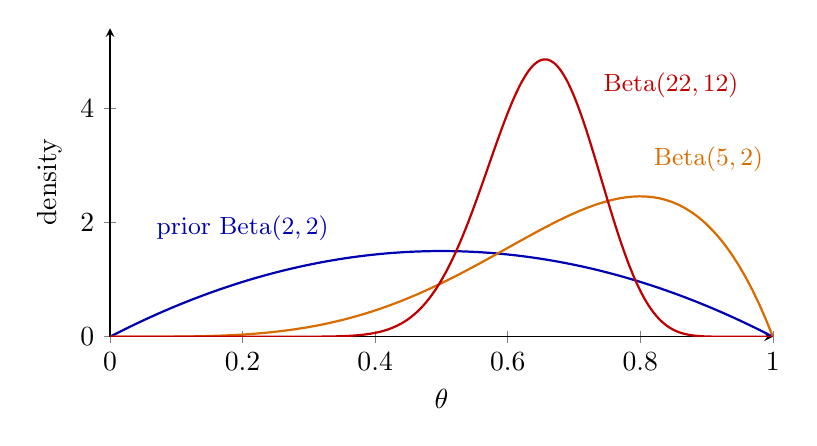
\begin{tikzpicture}
        \begin{axis}[width=10cm, height=5.5cm, xmin=0, xmax=1, ymin=0, ymax=5.4, axis lines=left, xlabel={$\theta$}, ylabel={density}, every axis plot/.append style={thick}]
            \addplot[blue!70!black, domain=0:1, samples=100] {6*x*(1-x)};
            \addplot[orange!85!black, domain=0:1, samples=100] {30*x^4*(1-x)};
            \addplot[red!75!black, smooth] coordinates {(0.00,0) (0.01,0.0000) (0.30,0.0009) (0.31,0.0015) (0.32,0.0025) (0.33,0.0040) (0.34,0.0064) (0.35,0.0099) (0.36,0.0151) (0.37,0.0226) (0.38,0.0332) (0.39,0.0479) (0.40,0.0679) (0.41,0.0948) (0.42,0.1304) (0.43,0.1765) (0.44,0.2354) (0.45,0.3095) (0.46,0.4013) (0.47,0.5132) (0.48,0.6476) (0.49,0.8064) (0.50,0.9913) (0.51,1.2031) (0.52,1.4418) (0.53,1.7063) (0.54,1.9943) (0.55,2.3022) (0.56,2.6249) (0.57,2.9560) (0.58,3.2879) (0.59,3.6116) (0.60,3.9176) (0.61,4.1959) (0.62,4.4364) (0.63,4.6297) (0.64,4.7675) (0.65,4.8430) (0.66,4.8515) (0.67,4.7908) (0.68,4.6615) (0.69,4.4668) (0.70,4.2129) (0.71,3.9083) (0.72,3.5637) (0.73,3.1913) (0.74,2.8039) (0.75,2.4144) (0.76,2.0351) (0.77,1.6769) (0.78,1.3484) (0.79,1.0563) (0.80,0.8043) (0.81,0.5938) (0.82,0.4239) (0.83,0.2916) (0.84,0.1925) (0.85,0.1213) (0.86,0.0726) (0.87,0.0410) (0.88,0.0216) (0.89,0.0105) (0.90,0.0047) (0.91,0.0018) (0.92,0.0006) (0.99,0.0000) (1.00,0)};
            \node[blue!70!black, font=\small] at (axis cs:0.2,1.9) {prior Beta$(2, 2)$};
            \node[orange!85!black, font=\small, left] at (axis cs:1.0,3.1) {Beta$(5, 2)$};
            \node[red!75!black, font=\small, right] at (axis cs:0.73,4.4) {Beta$(22, 12)$};
        \end{axis}
    \end{tikzpicture}
    \caption{Bayesian updating for the probability $\theta$ of heads: the prior Beta$(2, 2)$ (blue), the posterior Beta$(5, 2)$ after $3$ heads in $3$ flips (orange), and the posterior Beta$(22, 12)$ after $20$ heads in $30$ flips (red). With more data, the posterior concentrates around the relative frequency of heads.}
    \label{L4-fig:beta}
\end{figure}

To predict the next flip, Bayesian inference averages over all values of $\theta$, weighted by the posterior:
\[P(X_{N+1} = 1 \mid \mathcal{D}) = \int_0^1 \theta\,p(\theta \mid \mathcal{D}) \, d\theta = \E[\theta \mid \mathcal{D}] = \frac{a + k}{a + b + N}.\]
For the uniform prior ($a = b = 1$), this is Laplace's rule of succession $\frac{k + 1}{N + 2}$: after three heads in three flips, the probability of heads is $\frac{4}{5}$, not $1$. The same ``add pseudo-counts'' idea (Laplace smoothing) prevents zero probabilities for unseen words in language models.

\begin{example}[Credible intervals]\label{L4-ex:credible}
    A $95\%$ credible interval contains $\theta$ with posterior probability $0.95$, for example the interval between the $2.5\%$ and the $97.5\%$ quantiles of the posterior. For the posterior Beta$(22, 12)$ after $20$ heads in $30$ flips (Example~\ref{L4-ex:beta-coin}), it is $[0.48, 0.80]$ (computed numerically), close to the approximate confidence interval $\frac{2}{3} \pm 1.96\sqrt{\frac{2}{3} \cdot \frac{1}{3}/30} = [0.50, 0.84]$ of Section~\ref{L4-sec:estimation}. The interpretations differ: the credible interval makes a probability statement about $\theta$, given the data, while the confidence interval makes a probability statement about the random interval, for a fixed $\theta$. As the amount of data grows, the two intervals agree more and more (the Bernstein--von Mises theorem).
\end{example}

\begin{example}[Gamma--Poisson conjugacy]\label{L4-ex:gamma-poisson}
    Let the numbers of clicks on an ad in $N$ hours be i.i.d.\ Poisson$(\lambda)$, and let the prior of $\lambda$ be the Gamma distribution with the shape $a$ and the rate $b$, i.e., with the density $\frac{b^a}{\Gamma(a)}\lambda^{a-1}e^{-b\lambda}$ for $\lambda > 0$ and the mean $\frac{a}{b}$ (the Gamma distribution of Example~\ref{L4-ex:moments} with the scale $\frac{1}{b}$). If $S$ is the total number of clicks, the posterior is
    \[p(\lambda \mid \mathcal{D}) \propto e^{-N\lambda}\lambda^S \cdot \lambda^{a-1}e^{-b\lambda} = \lambda^{a + S - 1}e^{-(b + N)\lambda},\]
    i.e., Gamma$(a + S, b + N)$: the prior acts like $b$ previous hours with $a$ clicks in total. The posterior mean $\frac{a + S}{b + N}$ lies between the prior mean $\frac{a}{b}$ and the MLE $\frac{S}{N}$. For the prior Gamma$(2, 1)$ and the counts $3, 5, 4, 6, 2$ in five hours, the posterior is Gamma$(22, 6)$, with the mean $\frac{22}{6} \approx 3.67$ (the MLE is $4$) and the standard deviation $\frac{\sqrt{22}}{6} \approx 0.78$. The predictive probability of an hour without clicks is $\int e^{-\lambda}\,p(\lambda \mid \mathcal{D})\, d\lambda = \big(\frac{6}{7}\big)^{22} \approx 0.034$, while plugging in the MLE gives $e^{-4} \approx 0.018$: the posterior accounts for the uncertainty about $\lambda$.
\end{example}

\subsection{Maximum a posteriori estimation and regularization}

Often we only want a single parameter value. The maximum a posteriori (MAP) estimate is the mode of the posterior,
\[\hat\theta_{\text{MAP}} = \argmax_\theta p(\theta \mid \mathcal{D}) = \argmin_\theta \big(-\log p(\mathcal{D} \mid \theta) - \log p(\theta)\big),\]
since $p(\mathcal{D})$ does not depend on $\theta$. So MAP estimation minimizes the negative log-likelihood plus a penalty $-\log p(\theta)$ coming from the prior: a prior is a regularizer.

\begin{proposition}[Ridge regression as MAP estimation]\label{L4-prop:ridge-map}
    In the linear regression model of Proposition~\ref{L4-prop:ls-mle}, with the prior $\mathbf{w} \sim \mathcal{N}(\mathbf{0}, \alpha^{-1}I)$, the MAP estimate minimizes $\norm{\mathbf{y} - X\mathbf{w}}^2 + \lambda\norm{\mathbf{w}}^2$ with $\lambda = \alpha\sigma^2$, i.e., it is the ridge regression solution $\hat{\mathbf{w}} = (X^\top X + \lambda I)^{-1}X^\top\mathbf{y}$.
\end{proposition}

\begin{proof}
    Up to constants, $-\log p(\mathcal{D} \mid \mathbf{w}) - \log p(\mathbf{w}) = \frac{1}{2\sigma^2}\norm{\mathbf{y} - X\mathbf{w}}^2 + \frac{\alpha}{2}\norm{\mathbf{w}}^2$; multiply by $2\sigma^2$. The minimum was computed in the exercises of Lecture~3.
\end{proof}

A strong prior belief that the weights are small (large $\alpha$) means strong regularization. Similarly, the Laplace prior $p(\mathbf{w}) \propto e^{-\norm{\mathbf{w}}_1/b}$ leads to $\ell_1$ regularization (the lasso), which favors sparse weight vectors.

\subsection{Bayesian linear regression}

The MAP estimate discards the uncertainty that the posterior expresses. In linear regression with a Gaussian prior, the full posterior can be computed with the tools of Section~\ref{L4-sec:gaussian}.

\begin{theorem}[Posterior of Bayesian linear regression]\label{L4-thm:blr}
    In the model of Proposition~\ref{L4-prop:ls-mle} with the prior $\mathbf{w} \sim \mathcal{N}(\mathbf{0}, \alpha^{-1}I)$, the posterior is $\mathcal{N}(\mathbf{m}, S)$ with
    \[S = \big(\alpha I + \sigma^{-2}X^\top X\big)^{-1}, \qquad \mathbf{m} = \sigma^{-2}SX^\top\mathbf{y}.\]
    For a new input $\mathbf{x}_*$, the predictive distribution of $y_* = \mathbf{w}^\top\mathbf{x}_* + \varepsilon_*$ is $\mathcal{N}(\mathbf{m}^\top\mathbf{x}_*, \, \mathbf{x}_*^\top S\mathbf{x}_* + \sigma^2)$.
\end{theorem}

\begin{proof}
    Up to an additive constant that does not depend on $\mathbf{w}$,
    \[\log p(\mathbf{w} \mid \mathcal{D}) = -\frac{1}{2\sigma^2}\norm{\mathbf{y} - X\mathbf{w}}^2 - \frac{\alpha}{2}\norm{\mathbf{w}}^2 = -\frac{1}{2}\mathbf{w}^\top S^{-1}\mathbf{w} + \sigma^{-2}\mathbf{y}^\top X\mathbf{w} + \text{const}.\]
    Completing the square, this is $-\frac{1}{2}(\mathbf{w} - \mathbf{m})^\top S^{-1}(\mathbf{w} - \mathbf{m}) + \text{const}$, since the linear term of the latter is $\mathbf{m}^\top S^{-1}\mathbf{w} = \sigma^{-2}\mathbf{y}^\top X\mathbf{w}$. So the posterior density is proportional to the density of $\mathcal{N}(\mathbf{m}, S)$, hence equal to it. Given the data, $\mathbf{w}^\top\mathbf{x}_*$ is $\mathcal{N}(\mathbf{m}^\top\mathbf{x}_*, \mathbf{x}_*^\top S\mathbf{x}_*)$ by Corollary~\ref{L4-cor:gaussian-linear}, and adding the independent noise $\varepsilon_* \sim \mathcal{N}(0, \sigma^2)$ adds $\sigma^2$ to the variance.
\end{proof}

The posterior mean $\mathbf{m} = (X^\top X + \alpha\sigma^2 I)^{-1}X^\top\mathbf{y}$ is the ridge regression solution, which is also the MAP estimate (the mode and the mean of a Gaussian coincide). But the posterior also gives error bars: the predictive variance $\mathbf{x}_*^\top S\mathbf{x}_* + \sigma^2$ consists of the uncertainty about the weights, which shrinks as we collect more data, and the noise, which does not.

\begin{example}\label{L4-ex:blr}
    For the data $(1, 2), (2, 3), (3, 5)$, the model $y = wx + \varepsilon$ without intercept, $\alpha = 1$ and $\sigma^2 = 1$: $S = (1 + 1 + 4 + 9)^{-1} = \frac{1}{15}$ and $m = \frac{1}{15}(2 + 6 + 15) = \frac{23}{15} \approx 1.53$. At $x_* = 4$, the predictive distribution is $\mathcal{N}(6.13, \, \frac{16}{15} + 1) \approx \mathcal{N}(6.13, 2.07)$.
\end{example}

\subsection{Gaussian processes}\label{L4-sec:gp}

Bayesian linear regression puts a prior on the weights of a fixed set of features. A Gaussian process puts a prior directly on the unknown function.

\begin{definition}[Gaussian process]\label{L4-def:gp}
    A Gaussian process with mean function $m$ and covariance function (or kernel) $k$ is a random function $f$ such that for all points $\mathbf{x}_1, \ldots, \mathbf{x}_n$, the vector $(f(\mathbf{x}_1), \ldots, f(\mathbf{x}_n))$ is Gaussian with the mean vector $(m(\mathbf{x}_i))_i$ and the covariance matrix $K$ with entries $K_{ij} = k(\mathbf{x}_i, \mathbf{x}_j)$. We write $f \sim \mathcal{GP}(m, k)$.
\end{definition}

For this to make sense, every such matrix $K$ must be symmetric and positive semidefinite. This holds, for example, for $k(\mathbf{x}, \mathbf{x}') = \boldsymbol{\phi}(\mathbf{x})^\top\boldsymbol{\phi}(\mathbf{x}')$ with any feature map $\boldsymbol{\phi}$, since $K$ is then a Gram matrix (compare with the remark on kernels in Lecture~2).

\begin{example}\label{L4-ex:kernels}
    \begin{enumerate}
        \item (Linear kernel.) If $f(\mathbf{x}) = \mathbf{w}^\top\mathbf{x}$ with $\mathbf{w} \sim \mathcal{N}(\mathbf{0}, \alpha^{-1}I)$, then
        \[\Cov(f(\mathbf{x}), f(\mathbf{x}')) = \mathbf{x}^\top\Cov(\mathbf{w})\mathbf{x}' = \alpha^{-1}\mathbf{x}^\top\mathbf{x}'.\]
        So the prior of Bayesian linear regression is the Gaussian process with the kernel $k(\mathbf{x}, \mathbf{x}') = \alpha^{-1}\mathbf{x}^\top\mathbf{x}'$.
        \item (Squared exponential kernel.) $k(\mathbf{x}, \mathbf{x}') = \exp\big(-\frac{\norm{\mathbf{x} - \mathbf{x}'}^2}{2\ell^2}\big)$ gives smooth random functions, whose values at points closer than the length scale $\ell$ are strongly correlated. It corresponds to infinitely many features.
        \item (Brownian motion.) $k(s, t) = \min(s, t)$ for $s, t \geq 0$ is the covariance function of Brownian motion, a random function that we study in Section~\ref{L4-sec:sde}.
    \end{enumerate}
\end{example}

\begin{proposition}[Gaussian process regression]\label{L4-prop:gp-regression}
    Let $f \sim \mathcal{GP}(0, k)$, and let $y_i = f(\mathbf{x}_i) + \varepsilon_i$ for $i = 1, \ldots, N$, with i.i.d.\ noise $\varepsilon_i \sim \mathcal{N}(0, \sigma^2)$ independent of $f$. Let $K$ be the kernel matrix of the training inputs, and for a new input $\mathbf{x}_*$, let $\mathbf{k}_* = (k(\mathbf{x}_1, \mathbf{x}_*), \ldots, k(\mathbf{x}_N, \mathbf{x}_*))^\top$. Then, given the data,
    \[f(\mathbf{x}_*) \sim \mathcal{N}\big(\mathbf{k}_*^\top(K + \sigma^2 I)^{-1}\mathbf{y}, \ k(\mathbf{x}_*, \mathbf{x}_*) - \mathbf{k}_*^\top(K + \sigma^2 I)^{-1}\mathbf{k}_*\big).\]
\end{proposition}

\begin{proof}
    The vector $(\mathbf{y}, f(\mathbf{x}_*))$ is Gaussian with mean $\mathbf{0}$ and the covariance blocks $\Cov(\mathbf{y}) = K + \sigma^2 I$, $\Cov(\mathbf{y}, f(\mathbf{x}_*)) = \mathbf{k}_*$ and $\Var(f(\mathbf{x}_*)) = k(\mathbf{x}_*, \mathbf{x}_*)$; now apply Theorem~\ref{L4-thm:gaussian-conditional}.
\end{proof}

The posterior mean $\sum_i \alpha_i k(\mathbf{x}_i, \mathbf{x}_*)$ with $\boldsymbol{\alpha} = (K + \sigma^2 I)^{-1}\mathbf{y}$ is a combination of kernel functions centered at the data points; it is also the prediction of kernel ridge regression. The posterior variance does not depend on $\mathbf{y}$: it is small near the data, and it returns to the prior variance far away from them (Figure~\ref{L4-fig:gp}). For the linear kernel, the proposition reproduces the predictive distribution of Theorem~\ref{L4-thm:blr}.

\begin{example}\label{L4-ex:gp}
    With the squared exponential kernel ($\ell = 1$), $\sigma^2 = 0.1$, and the data $(0, 1)$ and $(1, 0)$: $K + \sigma^2 I = \begin{pmatrix} 1.1 & 0.607 \\ 0.607 & 1.1 \end{pmatrix}$, and at $x_* = 0.5$, $\mathbf{k}_* = (0.882, 0.882)^\top$. The posterior mean is $0.517$, and the posterior variance is $1 - \mathbf{k}_*^\top(K + \sigma^2 I)^{-1}\mathbf{k}_* \approx 0.087$; a new noisy observation at $x_*$ has the predictive variance $0.087 + 0.1 = 0.187$.
\end{example}

\begin{figure}[ht]
    \centering
    \begin{tikzpicture}
        \begin{axis}[width=11cm, height=5.5cm, xmin=-3, xmax=3, ymin=-2.3, ymax=2.5, axis lines=left, xlabel={$x$}, ylabel={$f(x)$}]
            \addplot[name path=upper, draw=none] coordinates {(-3.000,2.210) (-2.950,2.176) (-2.900,2.133) (-2.850,2.078) (-2.800,2.012) (-2.750,1.933) (-2.700,1.843) (-2.650,1.741) (-2.600,1.627) (-2.550,1.503) (-2.500,1.369) (-2.450,1.227) (-2.400,1.079) (-2.350,0.930) (-2.300,0.785) (-2.250,0.652) (-2.200,0.545) (-2.150,0.466) (-2.100,0.403) (-2.050,0.340) (-2.000,0.269) (-1.950,0.187) (-1.900,0.092) (-1.850,-0.014) (-1.800,-0.130) (-1.750,-0.253) (-1.700,-0.382) (-1.650,-0.510) (-1.600,-0.631) (-1.550,-0.737) (-1.500,-0.816) (-1.450,-0.862) (-1.400,-0.876) (-1.350,-0.867) (-1.300,-0.843) (-1.250,-0.808) (-1.200,-0.767) (-1.150,-0.722) (-1.100,-0.677) (-1.050,-0.633) (-1.000,-0.591) (-0.950,-0.554) (-0.900,-0.522) (-0.850,-0.495) (-0.800,-0.474) (-0.750,-0.459) (-0.700,-0.447) (-0.650,-0.438) (-0.600,-0.430) (-0.550,-0.419) (-0.500,-0.402) (-0.450,-0.372) (-0.400,-0.325) (-0.350,-0.258) (-0.300,-0.177) (-0.250,-0.091) (-0.200,-0.005) (-0.150,0.077) (-0.100,0.152) (-0.050,0.219) (0.000,0.279) (0.050,0.331) (0.100,0.379) (0.150,0.423) (0.200,0.469) (0.250,0.519) (0.300,0.578) (0.350,0.647) (0.400,0.724) (0.450,0.804) (0.500,0.884) (0.550,0.958) (0.600,1.024) (0.650,1.078) (0.700,1.118) (0.750,1.145) (0.800,1.157) (0.850,1.157) (0.900,1.148) (0.950,1.138) (1.000,1.139) (1.050,1.159) (1.100,1.198) (1.150,1.247) (1.200,1.300) (1.250,1.351) (1.300,1.398) (1.350,1.436) (1.400,1.465) (1.450,1.483) (1.500,1.488) (1.550,1.480) (1.600,1.457) (1.650,1.421) (1.700,1.369) (1.750,1.304) (1.800,1.224) (1.850,1.131) (1.900,1.026) (1.950,0.910) (2.000,0.784) (2.050,0.649) (2.100,0.507) (2.150,0.361) (2.200,0.212) (2.250,0.065) (2.300,-0.075) (2.350,-0.195) (2.400,-0.259) (2.450,-0.236) (2.500,-0.155) (2.550,-0.048) (2.600,0.071) (2.650,0.195) (2.700,0.321) (2.750,0.448) (2.800,0.572) (2.850,0.694) (2.900,0.812) (2.950,0.924) (3.000,1.031)};
            \addplot[name path=lower, draw=none] coordinates {(-3.000,-1.025) (-2.950,-0.925) (-2.900,-0.821) (-2.850,-0.714) (-2.800,-0.605) (-2.750,-0.495) (-2.700,-0.386) (-2.650,-0.280) (-2.600,-0.179) (-2.550,-0.083) (-2.500,0.004) (-2.450,0.079) (-2.400,0.141) (-2.350,0.186) (-2.300,0.208) (-2.250,0.199) (-2.200,0.148) (-2.150,0.053) (-2.100,-0.071) (-2.050,-0.207) (-2.000,-0.344) (-1.950,-0.476) (-1.900,-0.599) (-1.850,-0.711) (-1.800,-0.811) (-1.750,-0.898) (-1.700,-0.972) (-1.650,-1.035) (-1.600,-1.091) (-1.550,-1.147) (-1.500,-1.213) (-1.450,-1.293) (-1.400,-1.384) (-1.350,-1.477) (-1.300,-1.565) (-1.250,-1.641) (-1.200,-1.704) (-1.150,-1.749) (-1.100,-1.776) (-1.050,-1.785) (-1.000,-1.774) (-0.950,-1.744) (-0.900,-1.696) (-0.850,-1.631) (-0.800,-1.552) (-0.750,-1.458) (-0.700,-1.355) (-0.650,-1.243) (-0.600,-1.128) (-0.550,-1.012) (-0.500,-0.901) (-0.450,-0.802) (-0.400,-0.720) (-0.350,-0.658) (-0.300,-0.609) (-0.250,-0.566) (-0.200,-0.523) (-0.150,-0.476) (-0.100,-0.422) (-0.050,-0.360) (0.000,-0.291) (0.050,-0.214) (0.100,-0.132) (0.150,-0.047) (0.200,0.036) (0.250,0.115) (0.300,0.183) (0.350,0.240) (0.400,0.286) (0.450,0.324) (0.500,0.359) (0.550,0.393) (0.600,0.430) (0.650,0.469) (0.700,0.513) (0.750,0.560) (0.800,0.609) (0.850,0.659) (0.900,0.704) (0.950,0.736) (1.000,0.742) (1.050,0.714) (1.100,0.652) (1.150,0.565) (1.200,0.459) (1.250,0.340) (1.300,0.213) (1.350,0.081) (1.400,-0.054) (1.450,-0.187) (1.500,-0.316) (1.550,-0.440) (1.600,-0.556) (1.650,-0.661) (1.700,-0.755) (1.750,-0.835) (1.800,-0.901) (1.850,-0.951) (1.900,-0.985) (1.950,-1.004) (2.000,-1.005) (2.050,-0.991) (2.100,-0.962) (2.150,-0.919) (2.200,-0.863) (2.250,-0.799) (2.300,-0.730) (2.350,-0.671) (2.400,-0.657) (2.450,-0.718) (2.500,-0.828) (2.550,-0.953) (2.600,-1.080) (2.650,-1.203) (2.700,-1.320) (2.750,-1.430) (2.800,-1.530) (2.850,-1.622) (2.900,-1.705) (2.950,-1.778) (3.000,-1.842)};
            \addplot[blue!15] fill between[of=upper and lower];
            \addplot[blue!70!black, thick] coordinates {(-3.000,0.592) (-2.950,0.626) (-2.900,0.656) (-2.850,0.682) (-2.800,0.703) (-2.750,0.719) (-2.700,0.728) (-2.650,0.730) (-2.600,0.724) (-2.550,0.710) (-2.500,0.686) (-2.450,0.653) (-2.400,0.610) (-2.350,0.558) (-2.300,0.497) (-2.250,0.426) (-2.200,0.347) (-2.150,0.260) (-2.100,0.166) (-2.050,0.067) (-2.000,-0.037) (-1.950,-0.144) (-1.900,-0.253) (-1.850,-0.362) (-1.800,-0.470) (-1.750,-0.576) (-1.700,-0.677) (-1.650,-0.772) (-1.600,-0.861) (-1.550,-0.942) (-1.500,-1.015) (-1.450,-1.077) (-1.400,-1.130) (-1.350,-1.172) (-1.300,-1.204) (-1.250,-1.225) (-1.200,-1.235) (-1.150,-1.236) (-1.100,-1.227) (-1.050,-1.209) (-1.000,-1.183) (-0.950,-1.149) (-0.900,-1.109) (-0.850,-1.063) (-0.800,-1.013) (-0.750,-0.959) (-0.700,-0.901) (-0.650,-0.841) (-0.600,-0.779) (-0.550,-0.716) (-0.500,-0.652) (-0.450,-0.587) (-0.400,-0.522) (-0.350,-0.458) (-0.300,-0.393) (-0.250,-0.328) (-0.200,-0.264) (-0.150,-0.200) (-0.100,-0.135) (-0.050,-0.071) (0.000,-0.006) (0.050,0.058) (0.100,0.123) (0.150,0.188) (0.200,0.253) (0.250,0.317) (0.300,0.381) (0.350,0.443) (0.400,0.505) (0.450,0.564) (0.500,0.621) (0.550,0.676) (0.600,0.727) (0.650,0.773) (0.700,0.815) (0.750,0.852) (0.800,0.883) (0.850,0.908) (0.900,0.926) (0.950,0.937) (1.000,0.940) (1.050,0.937) (1.100,0.925) (1.150,0.906) (1.200,0.879) (1.250,0.846) (1.300,0.805) (1.350,0.758) (1.400,0.706) (1.450,0.648) (1.500,0.586) (1.550,0.520) (1.600,0.451) (1.650,0.380) (1.700,0.307) (1.750,0.234) (1.800,0.162) (1.850,0.090) (1.900,0.020) (1.950,-0.047) (2.000,-0.111) (2.050,-0.171) (2.100,-0.227) (2.150,-0.279) (2.200,-0.325) (2.250,-0.367) (2.300,-0.403) (2.350,-0.433) (2.400,-0.458) (2.450,-0.477) (2.500,-0.491) (2.550,-0.500) (2.600,-0.505) (2.650,-0.504) (2.700,-0.499) (2.750,-0.491) (2.800,-0.479) (2.850,-0.464) (2.900,-0.447) (2.950,-0.427) (3.000,-0.406)};
            \addplot[only marks, mark=*, mark size=1.8pt, red!75!black] coordinates {(-2.200,0.362) (-1.500,-1.034) (-0.400,-0.523) (0.300,0.378) (1.000,0.952) (2.400,-0.464)};
        \end{axis}
    \end{tikzpicture}
    \caption{Gaussian process regression with the squared exponential kernel ($\ell = 0.7$, $\sigma^2 = 0.01$) for six data points (red): the posterior mean (blue) and a band of $\pm 2$ posterior standard deviations. The uncertainty is small near the data and grows back to the prior standard deviation $1$ between and beyond them.}
    \label{L4-fig:gp}
\end{figure}

The hyperparameters, such as $\ell$ and $\sigma^2$, are usually chosen by maximizing the marginal likelihood $\log p(\mathbf{y}) = -\frac{1}{2}\mathbf{y}^\top(K + \sigma^2 I)^{-1}\mathbf{y} - \frac{1}{2}\log\det(K + \sigma^2 I) - \frac{N}{2}\log(2\pi)$, since $\mathbf{y} \sim \mathcal{N}(\mathbf{0}, K + \sigma^2 I)$; its gradient can be computed with the matrix calculus of Lecture~3. The cost of solving with the $N \times N$ matrix $K + \sigma^2 I$ grows like $N^3$, so exact Gaussian processes are limited to moderate data sets. Remarkably, one can show that neural networks with random weights become Gaussian processes in the limit of infinitely wide layers.

\begin{remark}[Beyond conjugate models]
    For most models, such as neural networks, the posterior has no closed form, and the evidence $p(\mathcal{D})$ is an intractable integral. Approximate methods include Markov chain Monte Carlo sampling (Section~\ref{L4-sec:markov}) and variational inference, which approximates the posterior by a simpler distribution by minimizing a Kullback--Leibler divergence (Section~\ref{L4-sec:information}).
\end{remark}

\section{Information Theory}\label{L4-sec:information}

Information theory measures uncertainty and the difference between distributions. Its quantities appear in machine learning as loss functions (cross-entropy), as regularizers (the KL term of variational autoencoders), and in the analysis of learning algorithms.

\begin{definition}[Entropy, cross-entropy and KL divergence]\label{L4-def:entropy}
    Let $p = (p_1, \ldots, p_K)$ and $q = (q_1, \ldots, q_K)$ be probability distributions on $\{1, \ldots, K\}$. The entropy of $p$, the cross-entropy of $q$ relative to $p$, and the Kullback--Leibler (KL) divergence of $q$ from $p$ are
    \[H(p) = -\sum_k p_k\log p_k, \qquad H(p, q) = -\sum_k p_k\log q_k, \qquad \KL(p \,\|\, q) = \sum_k p_k\log\frac{p_k}{q_k},\]
    with the conventions $0\log 0 = 0$ and $\KL(p \,\|\, q) = \infty$ if $q_k = 0 < p_k$ for some $k$.
\end{definition}

The number $-\log p_k$ measures the surprise of seeing the outcome $k$: rare outcomes are surprising. The entropy is the expected surprise. With $\log_2$ instead of $\log$, entropy is measured in bits, and it is the minimal average number of bits per symbol needed to encode outcomes of $p$ (Shannon's source coding theorem). A fair coin has entropy $1$ bit, a coin with $P(\text{heads}) = 0.9$ only $0.47$ bits, and a deterministic outcome $0$ bits. Clearly $H(p) \geq 0$, and
\[H(p, q) = H(p) + \KL(p \,\|\, q):\]
the cross-entropy is the average number of bits if we encode outcomes of $p$ with a code designed for $q$, and the KL divergence is the number of extra bits we pay for using the wrong distribution.

\begin{theorem}[Gibbs' inequality]\label{L4-thm:gibbs}
    $\KL(p \,\|\, q) \geq 0$, with equality if and only if $p = q$.
\end{theorem}

\begin{proof}
    We may assume $q_k > 0$ whenever $p_k > 0$. Let $T$ be the set of $k$ with $p_k > 0$, and let $R$ be the random variable that takes the value $\frac{q_k}{p_k}$ with probability $p_k$, for $k \in T$. By Jensen's inequality for the concave function $\log$ (Theorem~\ref{L4-thm:jensen}),
    \[-\KL(p \,\|\, q) = \sum_{k \in T} p_k\log\frac{q_k}{p_k} = \E[\log R] \leq \log\E[R] = \log\sum_{k \in T} q_k \leq \log 1 = 0.\]
    If equality holds, then $\sum_{k \in T} q_k = 1$, and equality holds in Jensen's inequality, which for the strictly concave $\log$ happens only if $R$ is constant; so $q_k = c\,p_k$ for $k \in T$ and $q_k = 0$ otherwise, and $c = 1$ since both sum to $1$.
\end{proof}

Two consequences: the cross-entropy $H(p, q)$ is minimal for $q = p$, and for the uniform distribution $u$ on $K$ outcomes, $0 \leq \KL(p \,\|\, u) = \log K - H(p)$, so $H(p) \leq \log K$: the uniform distribution has maximal entropy (compare with the exercise on maximum entropy in Lecture~3). The KL divergence is not a distance in the sense of Lecture~2, since it is not symmetric. For $p = (\frac{1}{2}, \frac{1}{2})$ and $q = (0.9, 0.1)$, $\KL(p \,\|\, q) \approx 0.511$ but $\KL(q \,\|\, p) \approx 0.368$.

\begin{theorem}[Maximum likelihood minimizes the KL divergence]\label{L4-thm:mle-kl}
    Let $x_1, \ldots, x_N \in \{1, \ldots, K\}$ be data with the empirical distribution $\hat p$, i.e., $\hat p_k$ is the fraction of data points equal to $k$, and let $q_\theta$ be a model distribution. Then
    \[\frac{1}{N}\sum_{i=1}^N \log q_\theta(x_i) = -H(\hat p, q_\theta) = -H(\hat p) - \KL(\hat p \,\|\, q_\theta).\]
    So maximizing the likelihood is the same as minimizing the cross-entropy $H(\hat p, q_\theta)$, and the same as minimizing $\KL(\hat p \,\|\, q_\theta)$.
\end{theorem}

\begin{proof}
    Grouping the data points by their values, $\frac{1}{N}\sum_i \log q_\theta(x_i) = \sum_k \hat p_k\log q_\theta(k) = -H(\hat p, q_\theta)$. The term $H(\hat p)$ does not depend on $\theta$.
\end{proof}

This is why the loss of classifiers is called the cross-entropy loss: for each training example, it is the cross-entropy between the one-hot distribution of the true label and the predicted distribution, and training fits the model distribution to the data in the sense of the KL divergence.

\paragraph{Continuous distributions.} For densities, the sums become integrals: the differential entropy is $h(p) = -\int p(x)\log p(x)\, dx$, and $\KL(p \,\|\, q) = \int p(x)\log\frac{p(x)}{q(x)}\, dx \geq 0$. The differential entropy of $\mathcal{N}(\mu, \sigma^2)$ is $\frac{1}{2}\log(2\pi e\sigma^2)$, and among all densities with variance $\sigma^2$, the Gaussian has the largest entropy.

\begin{example}[Maximum entropy]\label{L4-ex:max-entropy}
    Among the distributions on $\mathbb{R}$ with the variance $1$, the uniform distribution on $[-\sqrt{3}, \sqrt{3}]$ has the differential entropy $\log(2\sqrt{3}) \approx 1.24$, the Laplace distribution with the density $\frac{1}{\sqrt{2}}e^{-\sqrt{2}|x|}$ has $1 + \frac{1}{2}\log 2 \approx 1.35$, and $\mathcal{N}(0, 1)$ has the largest value, $\frac{1}{2}\log(2\pi e) \approx 1.42$ nats. In fact, for every density $p$ with mean $0$ and variance $1$, $\KL(p \,\|\, \mathcal{N}(0, 1)) = -h(p) + \E_p\big[\frac{1}{2}\log(2\pi) + \frac{X^2}{2}\big] = \frac{1}{2}\log(2\pi e) - h(p)$, which is nonnegative by Gibbs' inequality. This proves the maximum entropy property of the Gaussian, which is one justification for Gaussian noise models: they assume nothing beyond the variance.
\end{example}

\begin{proposition}[KL divergence between Gaussians]\label{L4-prop:kl-gaussian}
    For $p = \mathcal{N}(\mu_1, \sigma_1^2)$ and $q = \mathcal{N}(\mu_2, \sigma_2^2)$,
    \[\KL(p \,\|\, q) = \log\frac{\sigma_2}{\sigma_1} + \frac{\sigma_1^2 + (\mu_1 - \mu_2)^2}{2\sigma_2^2} - \frac{1}{2}.\]
\end{proposition}

\begin{proof}
    $\log\frac{p(x)}{q(x)} = \log\frac{\sigma_2}{\sigma_1} - \frac{(x - \mu_1)^2}{2\sigma_1^2} + \frac{(x - \mu_2)^2}{2\sigma_2^2}$. Take the expectation for $X \sim p$, using $\E[(X - \mu_1)^2] = \sigma_1^2$ and $\E[(X - \mu_2)^2] = \sigma_1^2 + (\mu_1 - \mu_2)^2$.
\end{proof}

In a variational autoencoder, each data point is encoded as a Gaussian $\mathcal{N}(\mu, \sigma^2)$ (in each latent dimension), and the loss contains the term $\KL\big(\mathcal{N}(\mu, \sigma^2) \,\|\, \mathcal{N}(0, 1)\big) = \frac{1}{2}(\mu^2 + \sigma^2 - 1 - \log\sigma^2)$, which keeps the codes close to a standard Gaussian. For example, for $\mu = 1$ and $\sigma = 2$, it is $\frac{1}{2}(4 - \log 4) \approx 1.31$.

\paragraph{Mutual information.} The mutual information of two random variables is the KL divergence between their joint distribution and the product of their marginals,
\[I(X; Y) = \KL\big(p(x, y) \,\|\, p_X(x)p_Y(y)\big) = \sum_{x, y} p(x, y)\log\frac{p(x, y)}{p_X(x)p_Y(y)}.\]
By Gibbs' inequality, $I(X; Y) \geq 0$, with equality if and only if $X$ and $Y$ are independent. Unlike the correlation, it detects every kind of dependence. For Example~\ref{L4-ex:joint-table}, $I(X; Y) \approx 0.086$ nats.

\section{Stochastic Differential Equations}\label{L4-sec:sde}

Markov chains (Section~\ref{L4-sec:markov}) move in discrete steps. Many random processes change continuously in time: the position of a particle in a fluid, the price of a stock, the parameters of a network during training with stochastic gradients, or the gradually noised images of a diffusion model. Stochastic differential equations (SDEs) describe such processes by adding random noise to ordinary differential equations (Section~\ref{L3-sec:ode}). The source of the noise is Brownian motion.

\begin{definition}[Brownian motion]\label{L4-def:brownian}
    A Brownian motion (or Wiener process) is a family of random variables $B(t)$, $t \geq 0$, with $B(0) = 0$, such that
    \begin{enumerate}
        \item for $0 \leq t_0 < t_1 < \cdots < t_k$, the increments $B(t_1) - B(t_0), \ldots, B(t_k) - B(t_{k-1})$ are independent;
        \item $B(t) - B(s) \sim \mathcal{N}(0, t - s)$ for $s < t$;
        \item the paths $t \mapsto B(t)$ are continuous.
    \end{enumerate}
\end{definition}

That such a process exists is a theorem of Norbert Wiener, which we do not prove. On the grid $t_k = kh$, Brownian motion is simulated exactly by the random walk $B(t_{k+1}) = B(t_k) + \sqrt{h}\,Z_k$ with i.i.d.\ $Z_k \sim \mathcal{N}(0, 1)$ (Figure~\ref{L4-fig:sde}). Conversely, by the central limit theorem, every random walk with many small independent steps looks like a Brownian motion from far away.

\begin{proposition}\label{L4-prop:brownian}
    $\E[B(t)] = 0$, $\Var(B(t)) = t$, and $\Cov(B(s), B(t)) = \min(s, t)$.
\end{proposition}

\begin{proof}
    The first two statements are property (2) with $s = 0$. For $s \leq t$, $\Cov(B(s), B(t)) = \Cov\big(B(s), B(s) + (B(t) - B(s))\big) = \Var(B(s)) + 0 = s$, since the increment $B(t) - B(s)$ is independent of $B(s) = B(s) - B(0)$.
\end{proof}

So Brownian motion is a Gaussian process with mean $0$ and covariance function $\min(s, t)$ (Section~\ref{L4-sec:gp}). Its typical displacement in a time $h$ is $\sqrt{h}$, which is much larger than $h$ for small $h$: the difference quotient $\frac{B(t + h) - B(t)}{h}$ has the variance $\frac{1}{h} \to \infty$. In fact, the paths of Brownian motion are continuous but nowhere differentiable, and ordinary calculus does not apply to them.

With the filtration $\mathcal{F}_s = \sigma(B(u) : u \leq s)$, the independence of the increments gives $\E[B(t) \mid \mathcal{F}_s] = B(s) + \E[B(t) - B(s)] = B(s)$ for $s \leq t$: Brownian motion is a martingale in continuous time (Section~\ref{L4-sec:martingales}), the continuous analogue of a fair random walk.

\begin{definition}[Stochastic differential equation]\label{L4-def:sde}
    An SDE $dX = \mu(X)\,dt + \sigma(X)\,dB$, with drift $\mu$ and diffusion coefficient $\sigma$, describes a process with $X(t) = X(0) + \int_0^t \mu(X(s))\, ds + \int_0^t \sigma(X(s))\, dB(s)$, where the last integral is a stochastic (It\^o) integral. Its Euler--Maruyama approximation with step $h$ is
    \[X_{k+1} = X_k + \mu(X_k)\,h + \sigma(X_k)\sqrt{h}\,Z_k, \qquad Z_k \sim \mathcal{N}(0, 1) \text{ i.i.d.}\]
\end{definition}

We do not define the stochastic integral; for our purposes, the Euler--Maruyama scheme, which converges to the solution as $h \to 0$, can serve as the definition. It is Euler's method for the ODE $x' = \mu(x)$ (Section~\ref{L3-sec:euler}), plus Gaussian noise whose standard deviation is proportional to $\sqrt{h}$, and it is a Markov chain with continuous states. For $\sigma = 0$, the SDE is an ODE.

\begin{example}[The Ornstein--Uhlenbeck process]\label{L4-ex:ou}
    The SDE $dX = -\theta X\,dt + \sigma\,dB$ with $\theta > 0$ pulls $X$ towards $0$ while the noise pushes it around. Its Euler--Maruyama approximation is $X_{k+1} = (1 - \theta h)X_k + \sigma\sqrt{h}\,Z_k$. Its mean satisfies $\E[X_{k+1}] = (1 - \theta h)\E[X_k]$, so it follows Euler's method for the ODE $x' = -\theta x$, with the solution $e^{-\theta t}X(0)$. If $X_k \sim \mathcal{N}(0, v)$ is independent of $Z_k$, then $X_{k+1} \sim \mathcal{N}\big(0, (1 - \theta h)^2v + \sigma^2h\big)$ by Corollary~\ref{L4-cor:gaussian-linear}. So for $0 < \theta h < 2$, the chain has the stationary distribution $\mathcal{N}(0, v_h)$ with
    \[v_h = \frac{\sigma^2h}{1 - (1 - \theta h)^2} = \frac{\sigma^2}{\theta(2 - \theta h)} \to \frac{\sigma^2}{2\theta} \qquad \text{as } h \to 0.\]
    For $\theta = 1$, $\sigma = \sqrt{2}$, the stationary distribution of the SDE is $\mathcal{N}(0, 1)$ (Figure~\ref{L4-fig:sde}); for $\theta = \sigma = 1$ and $h = 0.01$, $v_h \approx 0.5025$ instead of $0.5$.
\end{example}

\begin{figure}[ht]
    \centering
    \begin{tikzpicture}[x=1.2cm, y=0.48cm, >=Stealth]
        \draw[->, gray] (0,-6.2) -- (5.4,-6.2) node[right] {$t$};
        \draw[->, gray] (0,-6.2) -- (0,1.9) node[above] {$B(t)$};
        \draw[gray, dotted] (0,0) -- (5.2,0);
        \foreach \v in {-4,-2,0}
            \draw[gray] (0.06,\v) -- (-0.06,\v) node[left, font=\scriptsize] {$\v$};
        \foreach \v in {0,...,5}
            \draw[gray] (\v,-6.05) -- (\v,-6.35) node[below, font=\scriptsize] {$\v$};
        \draw[blue!70!black] plot coordinates {(0.00,0.000) (0.02,0.000) (0.04,0.042) (0.06,0.004) (0.08,-0.122) (0.10,-0.187) (0.12,-0.327) (0.14,-0.318) (0.16,-0.129) (0.18,-0.198) (0.20,-0.286) (0.22,-0.217) (0.24,-0.166) (0.26,-0.151) (0.28,-0.283) (0.30,-0.287) (0.32,-0.189) (0.34,-0.379) (0.36,-0.444) (0.38,-0.713) (0.40,-0.895) (0.42,-1.155) (0.44,-1.189) (0.46,-1.368) (0.48,-1.330) (0.50,-1.307) (0.52,-1.334) (0.54,-1.690) (0.56,-1.766) (0.58,-1.773) (0.60,-1.757) (0.62,-1.973) (0.64,-2.041) (0.66,-2.179) (0.68,-2.293) (0.70,-2.143) (0.72,-2.258) (0.74,-2.262) (0.76,-2.137) (0.78,-2.220) (0.80,-2.236) (0.82,-2.220) (0.84,-2.211) (0.86,-2.384) (0.88,-2.373) (0.90,-2.181) (0.92,-2.400) (0.94,-2.278) (0.96,-2.262) (0.98,-2.352) (1.00,-2.069) (1.02,-1.962) (1.04,-2.131) (1.06,-2.121) (1.08,-2.039) (1.10,-2.066) (1.12,-1.969) (1.14,-1.979) (1.16,-1.884) (1.18,-1.681) (1.20,-1.776) (1.22,-1.748) (1.24,-1.813) (1.26,-1.795) (1.28,-1.963) (1.30,-2.045) (1.32,-2.073) (1.34,-1.946) (1.36,-1.784) (1.38,-1.971) (1.40,-2.083) (1.42,-1.992) (1.44,-2.274) (1.46,-2.339) (1.48,-2.353) (1.50,-2.175) (1.52,-2.078) (1.54,-2.124) (1.56,-2.176) (1.58,-2.211) (1.60,-1.996) (1.62,-2.056) (1.64,-2.099) (1.66,-2.049) (1.68,-2.067) (1.70,-2.094) (1.72,-2.252) (1.74,-2.254) (1.76,-2.316) (1.78,-2.151) (1.80,-2.059) (1.82,-2.062) (1.84,-1.968) (1.86,-2.016) (1.88,-1.867) (1.90,-1.868) (1.92,-1.785) (1.94,-1.968) (1.96,-1.919) (1.98,-2.158) (2.00,-2.446) (2.02,-2.489) (2.04,-2.616) (2.06,-2.593) (2.08,-2.275) (2.10,-2.393) (2.12,-2.481) (2.14,-2.452) (2.16,-2.382) (2.18,-2.407) (2.20,-2.436) (2.22,-2.337) (2.24,-2.264) (2.26,-2.410) (2.28,-2.421) (2.30,-2.416) (2.32,-2.565) (2.34,-2.528) (2.36,-2.650) (2.38,-2.512) (2.40,-2.485) (2.42,-2.472) (2.44,-2.556) (2.46,-2.573) (2.48,-2.855) (2.50,-3.015) (2.52,-2.964) (2.54,-3.265) (2.56,-3.145) (2.58,-3.392) (2.60,-3.285) (2.62,-3.405) (2.64,-3.295) (2.66,-3.276) (2.68,-3.493) (2.70,-3.317) (2.72,-3.113) (2.74,-3.122) (2.76,-3.161) (2.78,-3.183) (2.80,-3.321) (2.82,-3.166) (2.84,-3.243) (2.86,-3.250) (2.88,-3.362) (2.90,-3.451) (2.92,-3.631) (2.94,-3.454) (2.96,-3.475) (2.98,-3.339) (3.00,-3.337) (3.02,-3.435) (3.04,-3.481) (3.06,-3.561) (3.08,-3.559) (3.10,-3.613) (3.12,-3.655) (3.14,-3.850) (3.16,-3.964) (3.18,-3.730) (3.20,-3.825) (3.22,-3.974) (3.24,-3.926) (3.26,-3.727) (3.28,-3.933) (3.30,-3.962) (3.32,-4.052) (3.34,-4.301) (3.36,-4.197) (3.38,-4.200) (3.40,-4.190) (3.42,-4.297) (3.44,-4.232) (3.46,-4.309) (3.48,-4.329) (3.50,-4.485) (3.52,-4.657) (3.54,-4.469) (3.56,-4.540) (3.58,-4.499) (3.60,-4.504) (3.62,-4.566) (3.64,-4.638) (3.66,-4.549) (3.68,-4.592) (3.70,-4.613) (3.72,-4.610) (3.74,-4.444) (3.76,-4.347) (3.78,-4.293) (3.80,-4.373) (3.82,-4.568) (3.84,-4.434) (3.86,-4.297) (3.88,-4.317) (3.90,-4.241) (3.92,-4.130) (3.94,-4.013) (3.96,-3.882) (3.98,-3.947) (4.00,-3.732) (4.02,-3.909) (4.04,-3.787) (4.06,-3.717) (4.08,-3.593) (4.10,-3.328) (4.12,-3.118) (4.14,-3.280) (4.16,-3.519) (4.18,-3.403) (4.20,-3.547) (4.22,-3.548) (4.24,-3.430) (4.26,-3.662) (4.28,-3.960) (4.30,-3.924) (4.32,-3.918) (4.34,-3.952) (4.36,-3.947) (4.38,-4.069) (4.40,-4.283) (4.42,-4.306) (4.44,-4.444) (4.46,-4.676) (4.48,-4.604) (4.50,-4.613) (4.52,-4.556) (4.54,-4.696) (4.56,-4.789) (4.58,-4.930) (4.60,-5.055) (4.62,-5.028) (4.64,-5.138) (4.66,-5.088) (4.68,-5.040) (4.70,-4.754) (4.72,-4.951) (4.74,-4.825) (4.76,-4.838) (4.78,-4.840) (4.80,-5.045) (4.82,-5.110) (4.84,-5.005) (4.86,-5.016) (4.88,-5.005) (4.90,-5.046) (4.92,-4.883) (4.94,-4.886) (4.96,-5.197) (4.98,-5.295) (5.00,-5.573)};
        \draw[red!70!black] plot coordinates {(0.00,0.000) (0.02,-0.460) (0.04,-0.535) (0.06,-0.346) (0.08,-0.340) (0.10,-0.505) (0.12,-0.638) (0.14,-0.479) (0.16,-0.456) (0.18,-0.449) (0.20,-0.457) (0.22,-0.452) (0.24,-0.338) (0.26,-0.260) (0.28,-0.229) (0.30,-0.376) (0.32,-0.304) (0.34,-0.401) (0.36,-0.246) (0.38,-0.426) (0.40,-0.445) (0.42,-0.447) (0.44,-0.634) (0.46,-0.390) (0.48,-0.184) (0.50,-0.249) (0.52,-0.140) (0.54,-0.087) (0.56,-0.456) (0.58,-0.421) (0.60,-0.430) (0.62,-0.418) (0.64,-0.570) (0.66,-0.608) (0.68,-0.633) (0.70,-0.465) (0.72,-0.418) (0.74,-0.419) (0.76,-0.203) (0.78,-0.281) (0.80,-0.336) (0.82,-0.593) (0.84,-0.371) (0.86,-0.235) (0.88,-0.105) (0.90,-0.011) (0.92,0.005) (0.94,0.035) (0.96,-0.000) (0.98,-0.029) (1.00,-0.021) (1.02,0.192) (1.04,0.271) (1.06,0.263) (1.08,0.181) (1.10,0.091) (1.12,0.318) (1.14,0.389) (1.16,0.399) (1.18,0.350) (1.20,0.193) (1.22,0.184) (1.24,0.307) (1.26,0.252) (1.28,0.220) (1.30,0.188) (1.32,0.204) (1.34,-0.021) (1.36,-0.055) (1.38,-0.176) (1.40,-0.050) (1.42,-0.159) (1.44,-0.078) (1.46,0.138) (1.48,0.093) (1.50,0.008) (1.52,0.035) (1.54,0.035) (1.56,-0.105) (1.58,-0.040) (1.60,0.245) (1.62,0.208) (1.64,0.180) (1.66,0.032) (1.68,0.077) (1.70,-0.099) (1.72,-0.256) (1.74,-0.075) (1.76,-0.203) (1.78,-0.050) (1.80,0.165) (1.82,0.202) (1.84,0.280) (1.86,0.557) (1.88,0.529) (1.90,0.445) (1.92,0.253) (1.94,0.259) (1.96,0.469) (1.98,0.604) (2.00,0.471) (2.02,0.350) (2.04,0.279) (2.06,0.320) (2.08,0.291) (2.10,0.321) (2.12,0.363) (2.14,0.321) (2.16,0.315) (2.18,0.345) (2.20,0.333) (2.22,0.404) (2.24,0.669) (2.26,0.752) (2.28,0.760) (2.30,0.522) (2.32,0.577) (2.34,0.301) (2.36,0.102) (2.38,0.223) (2.40,0.323) (2.42,0.302) (2.44,0.060) (2.46,0.007) (2.48,-0.089) (2.50,0.001) (2.52,0.321) (2.54,0.351) (2.56,0.241) (2.58,0.075) (2.60,0.068) (2.62,0.043) (2.64,-0.120) (2.66,-0.104) (2.68,-0.267) (2.70,-0.109) (2.72,0.041) (2.74,0.194) (2.76,0.127) (2.78,0.200) (2.80,0.181) (2.82,0.126) (2.84,0.078) (2.86,-0.105) (2.88,-0.310) (2.90,-0.197) (2.92,-0.224) (2.94,-0.194) (2.96,-0.052) (2.98,-0.297) (3.00,-0.408) (3.02,-0.383) (3.04,-0.328) (3.06,-0.381) (3.08,-0.236) (3.10,-0.206) (3.12,-0.377) (3.14,-0.509) (3.16,-0.395) (3.18,-0.330) (3.20,-0.598) (3.22,-0.407) (3.24,-0.323) (3.26,-0.133) (3.28,-0.187) (3.30,-0.229) (3.32,-0.388) (3.34,-0.030) (3.36,-0.054) (3.38,0.170) (3.40,0.079) (3.42,0.102) (3.44,-0.135) (3.46,-0.189) (3.48,-0.050) (3.50,-0.227) (3.52,-0.075) (3.54,-0.027) (3.56,-0.175) (3.58,-0.246) (3.60,-0.311) (3.62,-0.318) (3.64,-0.394) (3.66,-0.511) (3.68,-0.554) (3.70,-0.699) (3.72,-0.881) (3.74,-0.888) (3.76,-0.763) (3.78,-0.980) (3.80,-0.979) (3.82,-1.071) (3.84,-1.209) (3.86,-1.088) (3.88,-1.162) (3.90,-0.950) (3.92,-1.060) (3.94,-1.005) (3.96,-1.038) (3.98,-1.144) (4.00,-1.061) (4.02,-1.083) (4.04,-0.998) (4.06,-1.004) (4.08,-1.158) (4.10,-1.172) (4.12,-1.165) (4.14,-1.030) (4.16,-1.158) (4.18,-1.163) (4.20,-1.407) (4.22,-1.315) (4.24,-1.468) (4.26,-1.723) (4.28,-1.731) (4.30,-1.575) (4.32,-1.791) (4.34,-1.944) (4.36,-2.050) (4.38,-2.209) (4.40,-2.156) (4.42,-2.270) (4.44,-2.372) (4.46,-2.289) (4.48,-2.396) (4.50,-2.335) (4.52,-2.472) (4.54,-2.644) (4.56,-2.903) (4.58,-2.640) (4.60,-2.685) (4.62,-2.651) (4.64,-2.655) (4.66,-2.633) (4.68,-2.626) (4.70,-2.356) (4.72,-2.503) (4.74,-2.723) (4.76,-2.866) (4.78,-3.055) (4.80,-2.949) (4.82,-2.833) (4.84,-2.969) (4.86,-3.166) (4.88,-3.216) (4.90,-3.019) (4.92,-3.418) (4.94,-3.344) (4.96,-3.496) (4.98,-3.349) (5.00,-3.501)};
        \draw[orange!85!black] plot coordinates {(0.00,0.000) (0.02,-0.040) (0.04,-0.253) (0.06,-0.392) (0.08,-0.196) (0.10,-0.080) (0.12,-0.136) (0.14,-0.259) (0.16,-0.527) (0.18,-0.583) (0.20,-0.587) (0.22,-0.599) (0.24,-0.612) (0.26,-0.771) (0.28,-0.780) (0.30,-0.786) (0.32,-0.603) (0.34,-0.339) (0.36,-0.359) (0.38,-0.467) (0.40,-0.476) (0.42,-0.562) (0.44,-0.667) (0.46,-0.676) (0.48,-0.823) (0.50,-0.737) (0.52,-0.752) (0.54,-0.717) (0.56,-0.743) (0.58,-0.845) (0.60,-0.980) (0.62,-1.013) (0.64,-1.091) (0.66,-1.058) (0.68,-1.058) (0.70,-1.251) (0.72,-1.241) (0.74,-1.431) (0.76,-1.518) (0.78,-1.560) (0.80,-1.854) (0.82,-1.841) (0.84,-1.819) (0.86,-1.842) (0.88,-1.902) (0.90,-1.955) (0.92,-2.093) (0.94,-2.131) (0.96,-2.209) (0.98,-2.196) (1.00,-2.366) (1.02,-2.333) (1.04,-2.313) (1.06,-2.333) (1.08,-2.395) (1.10,-2.317) (1.12,-2.552) (1.14,-2.487) (1.16,-2.453) (1.18,-2.413) (1.20,-2.358) (1.22,-2.451) (1.24,-2.487) (1.26,-2.397) (1.28,-2.336) (1.30,-2.307) (1.32,-2.521) (1.34,-2.445) (1.36,-2.280) (1.38,-2.137) (1.40,-2.104) (1.42,-2.324) (1.44,-2.191) (1.46,-2.212) (1.48,-2.570) (1.50,-2.517) (1.52,-2.728) (1.54,-2.911) (1.56,-3.001) (1.58,-2.821) (1.60,-2.873) (1.62,-2.835) (1.64,-2.588) (1.66,-2.362) (1.68,-2.377) (1.70,-2.411) (1.72,-2.589) (1.74,-2.688) (1.76,-2.628) (1.78,-2.572) (1.80,-2.556) (1.82,-2.415) (1.84,-2.524) (1.86,-2.532) (1.88,-2.429) (1.90,-2.346) (1.92,-2.195) (1.94,-2.139) (1.96,-2.183) (1.98,-2.131) (2.00,-2.273) (2.02,-2.505) (2.04,-2.423) (2.06,-2.431) (2.08,-2.387) (2.10,-2.627) (2.12,-2.679) (2.14,-2.764) (2.16,-2.886) (2.18,-3.205) (2.20,-3.252) (2.22,-3.125) (2.24,-3.071) (2.26,-3.156) (2.28,-3.158) (2.30,-3.051) (2.32,-3.442) (2.34,-3.459) (2.36,-3.383) (2.38,-3.286) (2.40,-3.046) (2.42,-2.885) (2.44,-2.841) (2.46,-2.798) (2.48,-2.687) (2.50,-2.763) (2.52,-2.769) (2.54,-2.641) (2.56,-2.364) (2.58,-2.386) (2.60,-2.393) (2.62,-2.365) (2.64,-2.175) (2.66,-2.179) (2.68,-1.972) (2.70,-2.108) (2.72,-2.135) (2.74,-2.163) (2.76,-2.051) (2.78,-1.904) (2.80,-2.117) (2.82,-2.247) (2.84,-2.199) (2.86,-2.292) (2.88,-2.507) (2.90,-2.360) (2.92,-2.291) (2.94,-2.221) (2.96,-2.288) (2.98,-2.143) (3.00,-2.177) (3.02,-2.021) (3.04,-2.150) (3.06,-2.271) (3.08,-2.242) (3.10,-2.342) (3.12,-2.246) (3.14,-2.209) (3.16,-2.340) (3.18,-2.329) (3.20,-2.379) (3.22,-2.250) (3.24,-2.339) (3.26,-2.401) (3.28,-2.230) (3.30,-1.913) (3.32,-1.631) (3.34,-1.622) (3.36,-1.591) (3.38,-1.374) (3.40,-1.391) (3.42,-1.530) (3.44,-1.513) (3.46,-1.449) (3.48,-1.566) (3.50,-1.799) (3.52,-2.002) (3.54,-1.908) (3.56,-2.016) (3.58,-2.036) (3.60,-2.005) (3.62,-1.918) (3.64,-1.965) (3.66,-1.895) (3.68,-2.021) (3.70,-2.072) (3.72,-2.217) (3.74,-2.057) (3.76,-2.060) (3.78,-2.165) (3.80,-2.215) (3.82,-2.246) (3.84,-2.147) (3.86,-2.373) (3.88,-2.519) (3.90,-2.573) (3.92,-2.215) (3.94,-2.080) (3.96,-2.095) (3.98,-1.995) (4.00,-1.704) (4.02,-1.737) (4.04,-1.789) (4.06,-1.617) (4.08,-1.547) (4.10,-1.452) (4.12,-1.524) (4.14,-1.252) (4.16,-1.010) (4.18,-0.930) (4.20,-0.834) (4.22,-1.120) (4.24,-1.030) (4.26,-1.058) (4.28,-0.996) (4.30,-0.900) (4.32,-0.948) (4.34,-1.187) (4.36,-1.135) (4.38,-1.240) (4.40,-1.287) (4.42,-1.372) (4.44,-1.420) (4.46,-1.747) (4.48,-1.575) (4.50,-1.539) (4.52,-1.382) (4.54,-1.102) (4.56,-1.099) (4.58,-1.354) (4.60,-1.480) (4.62,-1.651) (4.64,-1.722) (4.66,-1.710) (4.68,-1.993) (4.70,-1.945) (4.72,-2.159) (4.74,-2.117) (4.76,-2.132) (4.78,-2.176) (4.80,-2.187) (4.82,-2.263) (4.84,-2.350) (4.86,-2.588) (4.88,-2.592) (4.90,-2.331) (4.92,-2.051) (4.94,-1.864) (4.96,-1.764) (4.98,-1.860) (5.00,-1.656)};
    \end{tikzpicture}
    \quad
    \begin{tikzpicture}[x=1.2cm, y=0.62cm, >=Stealth]
        \draw[->, gray] (0,-3.2) -- (5.4,-3.2) node[right] {$t$};
        \draw[->, gray] (0,-3.2) -- (0,3.3) node[above] {$X(t)$};
        \foreach \v in {-2,0,2} {
            \draw[gray, dotted] (0,\v) -- (5.2,\v);
            \draw[gray] (0.06,\v) -- (-0.06,\v) node[left, font=\scriptsize] {$\v$};
        }
        \foreach \v in {0,...,5}
            \draw[gray] (\v,-3.08) -- (\v,-3.32) node[below, font=\scriptsize] {$\v$};
        \draw[blue!70!black, dashed, thin] plot[domain=0:5, samples=60] (\x, {2.5*exp(-\x)});
        \draw[red!70!black, dashed, thin] plot[domain=0:5, samples=60] (\x, {-2.0*exp(-\x)});
        \draw[orange!85!black, dashed, thin] plot[domain=0:5, samples=60] (\x, {0*exp(-\x)});
        \draw[blue!70!black] plot coordinates {(0.00,2.500) (0.02,2.439) (0.04,2.376) (0.06,2.270) (0.08,2.243) (0.10,2.112) (0.12,2.053) (0.14,1.795) (0.16,1.684) (0.18,2.106) (0.20,2.050) (0.22,1.962) (0.24,2.029) (0.26,2.130) (0.28,1.865) (0.30,1.786) (0.32,1.934) (0.34,1.949) (0.36,1.934) (0.38,2.207) (0.40,2.027) (0.42,2.003) (0.44,1.859) (0.46,2.120) (0.48,1.687) (0.50,1.519) (0.52,1.383) (0.54,1.488) (0.56,1.580) (0.58,1.827) (0.60,1.476) (0.62,1.596) (0.64,1.506) (0.66,1.342) (0.68,1.423) (0.70,1.211) (0.72,0.771) (0.74,0.682) (0.76,0.369) (0.78,0.232) (0.80,0.301) (0.82,0.358) (0.84,0.668) (0.86,0.615) (0.88,0.296) (0.90,0.138) (0.92,-0.048) (0.94,-0.291) (0.96,-0.198) (0.98,-0.323) (1.00,-0.712) (1.02,-0.558) (1.04,-0.570) (1.06,-0.487) (1.08,-0.456) (1.10,-0.320) (1.12,-0.306) (1.14,-0.053) (1.16,0.033) (1.18,0.111) (1.20,0.191) (1.22,-0.105) (1.24,-0.135) (1.26,-0.185) (1.28,-0.139) (1.30,-0.408) (1.32,-0.073) (1.34,-0.051) (1.36,-0.292) (1.38,-0.628) (1.40,-0.672) (1.42,-0.676) (1.44,-0.807) (1.46,-0.772) (1.48,-0.885) (1.50,-0.757) (1.52,-0.887) (1.54,-0.876) (1.56,-0.663) (1.58,-0.136) (1.60,-0.334) (1.62,-0.421) (1.64,-0.580) (1.66,-0.412) (1.68,-0.633) (1.70,-0.717) (1.72,-0.709) (1.74,-0.890) (1.76,-1.064) (1.78,-1.138) (1.80,-1.535) (1.82,-1.794) (1.84,-1.840) (1.86,-1.774) (1.88,-1.776) (1.90,-2.095) (1.92,-2.146) (1.94,-1.943) (1.96,-1.793) (1.98,-1.773) (2.00,-1.915) (2.02,-1.750) (2.04,-1.831) (2.06,-2.028) (2.08,-2.148) (2.10,-1.816) (2.12,-1.735) (2.14,-1.469) (2.16,-1.535) (2.18,-1.317) (2.20,-1.411) (2.22,-1.414) (2.24,-0.889) (2.26,-0.717) (2.28,-0.803) (2.30,-0.804) (2.32,-0.723) (2.34,-0.466) (2.36,-0.555) (2.38,-0.892) (2.40,-0.930) (2.42,-0.908) (2.44,-0.868) (2.46,-0.588) (2.48,-0.513) (2.50,-0.340) (2.52,-0.553) (2.54,-0.368) (2.56,0.058) (2.58,0.212) (2.60,0.258) (2.62,0.284) (2.64,0.635) (2.66,0.437) (2.68,0.406) (2.70,0.490) (2.72,0.629) (2.74,0.529) (2.76,0.580) (2.78,0.513) (2.80,0.527) (2.82,0.490) (2.84,0.252) (2.86,0.242) (2.88,0.413) (2.90,0.211) (2.92,0.159) (2.94,0.289) (2.96,0.069) (2.98,0.104) (3.00,-0.110) (3.02,0.119) (3.04,0.579) (3.06,0.972) (3.08,0.909) (3.10,1.039) (3.12,1.042) (3.14,1.042) (3.16,1.330) (3.18,1.040) (3.20,1.230) (3.22,1.196) (3.24,1.454) (3.26,1.462) (3.28,1.298) (3.30,1.328) (3.32,1.448) (3.34,1.427) (3.36,1.496) (3.38,1.361) (3.40,0.907) (3.42,1.069) (3.44,1.188) (3.46,1.194) (3.48,1.183) (3.50,1.367) (3.52,1.248) (3.54,1.082) (3.56,1.023) (3.58,1.240) (3.60,0.938) (3.62,1.157) (3.64,1.006) (3.66,0.766) (3.68,1.003) (3.70,0.963) (3.72,0.684) (3.74,0.599) (3.76,0.773) (3.78,0.996) (3.80,0.890) (3.82,0.954) (3.84,1.078) (3.86,0.927) (3.88,0.980) (3.90,0.954) (3.92,0.827) (3.94,0.712) (3.96,0.712) (3.98,0.703) (4.00,0.576) (4.02,0.479) (4.04,0.692) (4.06,0.721) (4.08,0.884) (4.10,1.107) (4.12,1.202) (4.14,1.632) (4.16,1.435) (4.18,1.568) (4.20,1.473) (4.22,1.814) (4.24,2.118) (4.26,1.685) (4.28,1.458) (4.30,1.561) (4.32,1.688) (4.34,1.802) (4.36,1.751) (4.38,1.807) (4.40,1.902) (4.42,1.848) (4.44,2.017) (4.46,1.524) (4.48,1.621) (4.50,1.382) (4.52,1.546) (4.54,1.469) (4.56,1.262) (4.58,1.311) (4.60,1.103) (4.62,0.898) (4.64,0.567) (4.66,0.550) (4.68,0.639) (4.70,0.830) (4.72,0.785) (4.74,0.979) (4.76,0.963) (4.78,0.925) (4.80,1.022) (4.82,1.213) (4.84,1.120) (4.86,1.049) (4.88,0.996) (4.90,0.993) (4.92,0.793) (4.94,0.982) (4.96,0.883) (4.98,0.958) (5.00,0.773)};
        \draw[red!70!black] plot coordinates {(0.00,-2.000) (0.02,-1.888) (0.04,-1.772) (0.06,-1.821) (0.08,-1.380) (0.10,-1.278) (0.12,-0.897) (0.14,-0.688) (0.16,-0.806) (0.18,-0.867) (0.20,-0.762) (0.22,-0.735) (0.24,-0.710) (0.26,-0.753) (0.28,-1.100) (0.30,-1.123) (0.32,-1.544) (0.34,-1.439) (0.36,-1.555) (0.38,-1.667) (0.40,-1.678) (0.42,-1.590) (0.44,-1.844) (0.46,-2.157) (0.48,-2.327) (0.50,-2.689) (0.52,-2.829) (0.54,-2.454) (0.56,-2.616) (0.58,-2.433) (0.60,-2.659) (0.62,-2.546) (0.64,-2.559) (0.66,-2.520) (0.68,-2.356) (0.70,-1.957) (0.72,-1.879) (0.74,-1.817) (0.76,-1.975) (0.78,-1.819) (0.80,-1.832) (0.82,-1.629) (0.84,-1.605) (0.86,-1.225) (0.88,-1.597) (0.90,-1.624) (0.92,-1.415) (0.94,-1.457) (0.96,-1.586) (0.98,-1.608) (1.00,-1.852) (1.02,-1.791) (1.04,-1.267) (1.06,-1.013) (1.08,-1.214) (1.10,-1.365) (1.12,-1.418) (1.14,-1.189) (1.16,-1.330) (1.18,-1.441) (1.20,-1.235) (1.22,-1.038) (1.24,-1.092) (1.26,-1.293) (1.28,-1.577) (1.30,-1.686) (1.32,-2.098) (1.34,-1.906) (1.36,-1.994) (1.38,-1.858) (1.40,-1.447) (1.42,-1.184) (1.44,-1.390) (1.46,-1.188) (1.48,-0.933) (1.50,-1.064) (1.52,-1.233) (1.54,-1.230) (1.56,-1.526) (1.58,-1.201) (1.60,-1.658) (1.62,-1.847) (1.64,-1.864) (1.66,-1.872) (1.68,-1.801) (1.70,-1.711) (1.72,-1.719) (1.74,-1.457) (1.76,-1.856) (1.78,-1.819) (1.80,-1.926) (1.82,-1.861) (1.84,-1.779) (1.86,-1.926) (1.88,-2.016) (1.90,-1.817) (1.92,-1.711) (1.94,-1.813) (1.96,-1.368) (1.98,-0.879) (2.00,-1.154) (2.02,-1.071) (2.04,-0.547) (2.06,-0.380) (2.08,-0.328) (2.10,-0.363) (2.12,-0.464) (2.14,-0.497) (2.16,-0.597) (2.18,-0.436) (2.20,-0.507) (2.22,-0.585) (2.24,-0.814) (2.26,-0.808) (2.28,-0.970) (2.30,-0.987) (2.32,-0.759) (2.34,-0.671) (2.36,-0.556) (2.38,-0.474) (2.40,-0.453) (2.42,-0.469) (2.44,-0.521) (2.46,-0.359) (2.48,-0.569) (2.50,-0.289) (2.52,-0.277) (2.54,-0.421) (2.56,-0.510) (2.58,-0.635) (2.60,-0.591) (2.62,-0.722) (2.64,-0.480) (2.66,-0.626) (2.68,-1.068) (2.70,-1.193) (2.72,-1.571) (2.74,-1.547) (2.76,-1.305) (2.78,-1.149) (2.80,-1.394) (2.82,-1.518) (2.84,-1.132) (2.86,-1.046) (2.88,-1.024) (2.90,-0.792) (2.92,-0.286) (2.94,-0.021) (2.96,0.007) (2.98,0.078) (3.00,0.200) (3.02,0.074) (3.04,-0.140) (3.06,-0.126) (3.08,-0.313) (3.10,-0.319) (3.12,-0.294) (3.14,0.180) (3.16,0.007) (3.18,-0.018) (3.20,-0.050) (3.22,0.038) (3.24,0.247) (3.26,0.144) (3.28,-0.024) (3.30,-0.351) (3.32,-0.529) (3.34,-0.412) (3.36,-0.394) (3.38,-0.589) (3.40,-0.652) (3.42,-0.633) (3.44,-0.519) (3.46,-0.628) (3.48,-0.665) (3.50,-1.016) (3.52,-1.226) (3.54,-0.878) (3.56,-1.298) (3.58,-1.339) (3.60,-1.269) (3.62,-1.318) (3.64,-1.453) (3.66,-1.437) (3.68,-1.409) (3.70,-1.397) (3.72,-1.745) (3.74,-1.739) (3.76,-1.875) (3.78,-1.948) (3.80,-1.863) (3.82,-1.698) (3.84,-1.484) (3.86,-1.554) (3.88,-1.338) (3.90,-1.077) (3.92,-0.828) (3.94,-0.533) (3.96,-0.552) (3.98,-0.576) (4.00,-0.399) (4.02,-0.664) (4.04,-0.609) (4.06,-0.703) (4.08,-0.763) (4.10,-1.096) (4.12,-1.252) (4.14,-1.231) (4.16,-1.029) (4.18,-0.810) (4.20,-0.810) (4.22,-0.832) (4.24,-0.981) (4.26,-0.881) (4.28,-0.913) (4.30,-0.774) (4.32,-0.408) (4.34,-0.406) (4.36,-0.697) (4.38,-0.856) (4.40,-1.130) (4.42,-1.347) (4.44,-1.059) (4.46,-0.992) (4.48,-1.277) (4.50,-1.120) (4.52,-0.846) (4.54,-0.901) (4.56,-1.018) (4.58,-1.065) (4.60,-0.987) (4.62,-0.839) (4.64,-0.586) (4.66,-0.332) (4.68,-0.088) (4.70,0.186) (4.72,0.315) (4.74,0.002) (4.76,-0.024) (4.78,0.039) (4.80,-0.038) (4.82,0.145) (4.84,0.070) (4.86,-0.117) (4.88,0.174) (4.90,0.304) (4.92,0.342) (4.94,0.520) (4.96,0.723) (4.98,0.776) (5.00,0.269)};
        \draw[orange!85!black] plot coordinates {(0.00,0.000) (0.02,-0.135) (0.04,-0.224) (0.06,-0.416) (0.08,-0.368) (0.10,-0.122) (0.12,-0.217) (0.14,-0.439) (0.16,-0.025) (0.18,-0.115) (0.20,-0.359) (0.22,-0.304) (0.24,-0.213) (0.26,-0.350) (0.28,-0.185) (0.30,-0.279) (0.32,-0.458) (0.34,-0.413) (0.36,-0.250) (0.38,-0.372) (0.40,-0.299) (0.42,-0.311) (0.44,0.260) (0.46,0.113) (0.48,0.388) (0.50,0.369) (0.52,0.337) (0.54,0.474) (0.56,0.643) (0.58,0.884) (0.60,0.932) (0.62,0.793) (0.64,0.670) (0.66,0.758) (0.68,0.859) (0.70,1.122) (0.72,1.183) (0.74,1.372) (0.76,1.647) (0.78,1.647) (0.80,1.317) (0.82,1.055) (0.84,0.747) (0.86,1.050) (0.88,0.859) (0.90,1.089) (0.92,1.184) (0.94,1.503) (0.96,1.674) (0.98,1.620) (1.00,1.548) (1.02,1.534) (1.04,1.538) (1.06,1.401) (1.08,1.367) (1.10,1.661) (1.12,1.287) (1.14,1.313) (1.16,1.106) (1.18,1.121) (1.20,1.267) (1.22,1.230) (1.24,1.360) (1.26,1.015) (1.28,1.216) (1.30,1.071) (1.32,1.174) (1.34,1.187) (1.36,0.646) (1.38,0.482) (1.40,0.516) (1.42,0.817) (1.44,0.858) (1.46,0.892) (1.48,0.592) (1.50,0.866) (1.52,1.210) (1.54,1.192) (1.56,1.124) (1.58,0.778) (1.60,0.939) (1.62,1.461) (1.64,1.575) (1.66,1.796) (1.68,1.869) (1.70,1.634) (1.72,1.869) (1.74,1.585) (1.76,1.511) (1.78,1.536) (1.80,1.682) (1.82,1.732) (1.84,1.774) (1.86,1.587) (1.88,1.297) (1.90,1.283) (1.92,1.116) (1.94,0.832) (1.96,0.562) (1.98,0.453) (2.00,0.073) (2.02,-0.198) (2.04,-0.521) (2.06,-0.474) (2.08,-0.383) (2.10,0.026) (2.12,-0.274) (2.14,-0.404) (2.16,-0.214) (2.18,-0.253) (2.20,-0.313) (2.22,0.035) (2.24,-0.033) (2.26,-0.264) (2.28,-0.522) (2.30,-0.445) (2.32,-0.375) (2.34,-0.641) (2.36,-0.826) (2.38,-0.702) (2.40,-0.573) (2.42,-0.690) (2.44,-0.552) (2.46,-0.426) (2.48,-0.774) (2.50,-0.821) (2.52,-0.722) (2.54,-0.822) (2.56,-1.233) (2.58,-1.265) (2.60,-1.090) (2.62,-0.752) (2.64,-1.175) (2.66,-0.629) (2.68,-0.842) (2.70,-0.633) (2.72,-0.374) (2.74,-0.170) (2.76,-0.136) (2.78,-0.366) (2.80,-0.233) (2.82,-0.372) (2.84,-0.869) (2.86,-0.286) (2.88,-0.138) (2.90,0.228) (2.92,0.041) (2.94,0.334) (2.96,0.645) (2.98,0.943) (3.00,0.920) (3.02,0.661) (3.04,0.612) (3.06,0.160) (3.08,-0.184) (3.10,-0.162) (3.12,-0.357) (3.14,-0.383) (3.16,-0.397) (3.18,-0.003) (3.20,0.257) (3.22,0.243) (3.24,0.480) (3.26,0.314) (3.28,0.240) (3.30,0.418) (3.32,0.161) (3.34,0.102) (3.36,-0.164) (3.38,-0.137) (3.40,0.192) (3.42,0.038) (3.44,0.082) (3.46,-0.099) (3.48,-0.327) (3.50,-0.568) (3.52,-0.265) (3.54,0.212) (3.56,0.305) (3.58,0.155) (3.60,0.293) (3.62,0.221) (3.64,0.376) (3.66,0.427) (3.68,0.475) (3.70,0.586) (3.72,0.459) (3.74,0.369) (3.76,0.017) (3.78,-0.072) (3.80,-0.355) (3.82,-0.376) (3.84,-0.560) (3.86,-0.529) (3.88,-0.428) (3.90,-0.703) (3.92,-0.852) (3.94,-1.023) (3.96,-0.854) (3.98,-0.495) (4.00,-0.315) (4.02,-0.379) (4.04,-0.078) (4.06,-0.379) (4.08,-0.072) (4.10,-0.202) (4.12,-0.754) (4.14,-0.208) (4.16,0.111) (4.18,-0.097) (4.20,-0.062) (4.22,-0.103) (4.24,-0.081) (4.26,-0.376) (4.28,-0.505) (4.30,-0.401) (4.32,-0.348) (4.34,-0.102) (4.36,-0.084) (4.38,0.388) (4.40,0.237) (4.42,0.284) (4.44,-0.105) (4.46,-0.353) (4.48,-0.081) (4.50,-0.267) (4.52,-0.156) (4.54,-0.165) (4.56,-0.371) (4.58,-0.433) (4.60,-0.527) (4.62,-0.614) (4.64,-0.451) (4.66,-0.312) (4.68,-0.421) (4.70,-0.594) (4.72,-0.526) (4.74,-0.535) (4.76,-0.319) (4.78,0.219) (4.80,0.383) (4.82,0.368) (4.84,0.327) (4.86,0.149) (4.88,-0.036) (4.90,-0.236) (4.92,-0.310) (4.94,-0.389) (4.96,-0.233) (4.98,-0.308) (5.00,-0.341)};
    \end{tikzpicture}
    \caption{Left: three paths of Brownian motion, simulated with $h = 0.02$. Right: three paths of the Ornstein--Uhlenbeck process $dX = -X\,dt + \sqrt{2}\,dB$, started at $2.5$, $-2$ and $0$, together with the solutions $X(0)e^{-t}$ of the ODE without noise (dashed). The process forgets its starting point and fluctuates around $0$ with the stationary distribution $\mathcal{N}(0, 1)$; about $95\%$ of the time, it stays between $-2$ and $2$.}
    \label{L4-fig:sde}
\end{figure}

\subsection{Langevin dynamics and diffusion models}\label{L4-sec:langevin}

The Ornstein--Uhlenbeck process is an example of a general principle: a gradient flow with the right amount of noise samples from a probability distribution.

\begin{theorem}[Langevin dynamics]\label{L4-thm:langevin}
    Let $U: \mathbb{R}^d \to \mathbb{R}$ be smooth with $\int e^{-U(\mathbf{x})}\, d\mathbf{x} < \infty$. Then the SDE $d\mathbf{X} = -\nabla U(\mathbf{X})\,dt + \sqrt{2}\,d\mathbf{B}$, where $\mathbf{B}$ is a vector of $d$ independent Brownian motions, has the stationary density $p(\mathbf{x}) \propto e^{-U(\mathbf{x})}$, and under mild conditions, the distribution of $\mathbf{X}(t)$ converges to it.
\end{theorem}

We do not prove the convergence, but we can see why $e^{-U}$ is stationary. Without noise, the density $p_t$ of $\mathbf{X}(t)$ under the flow of the vector field $-\nabla U$ satisfies the continuity equation $\frac{\partial p_t}{\partial t} = -\Div(-p_t\nabla U)$ (Proposition~\ref{L3-prop:continuity}). The noise adds a diffusion term, and one can show that $p_t$ satisfies the Fokker--Planck equation
\[\frac{\partial p_t}{\partial t} = \Div(p_t\nabla U) + \Delta p_t = \Div(p_t\nabla U + \nabla p_t),\]
with the Laplacian $\Delta p_t = \Div\nabla p_t$ (Lecture~3). For $p \propto e^{-U}$, we have $\nabla p = -p\nabla U$, so the right side vanishes, and $p$ does not change in time. For $U = 0$, the Fokker--Planck equation is the heat equation $\frac{\partial p_t}{\partial t} = \Delta p_t$, which describes how the density of $\sqrt{2}\,\mathbf{B}(t)$ spreads out. For $U(x) = \frac{x^2}{2s^2}$, the SDE is the Ornstein--Uhlenbeck process with $\theta = \frac{1}{s^2}$ and $\sigma = \sqrt{2}$, whose stationary variance $\frac{\sigma^2}{2\theta} = s^2$ agrees with the density $e^{-U} \propto e^{-x^2/(2s^2)}$ of $\mathcal{N}(0, s^2)$. The Euler--Maruyama scheme gives the unadjusted Langevin algorithm
\[\mathbf{x}_{k+1} = \mathbf{x}_k - h\nabla U(\mathbf{x}_k) + \sqrt{2h}\,\mathbf{z}_k, \qquad \mathbf{z}_k \sim \mathcal{N}(\mathbf{0}, I),\]
which is gradient descent on $U$ plus Gaussian noise. To sample from a posterior $p(\boldsymbol{\theta} \mid \mathcal{D}) \propto e^{-U(\boldsymbol{\theta})}$, we take $U(\boldsymbol{\theta}) = -\log p(\mathcal{D} \mid \boldsymbol{\theta}) - \log p(\boldsymbol{\theta})$, the training loss plus the regularizer. Without the noise, the iteration converges to the MAP estimate; with the noise, it explores the posterior. The discretization introduces a small bias: for the target $\mathcal{N}(2, 0.25)$ and $h = 0.01$, the stationary variance of the algorithm is $0.2551$ instead of $0.25$, by Example~\ref{L4-ex:ou}. The Metropolis-adjusted Langevin algorithm removes this bias by accepting or rejecting each step as in Theorem~\ref{L4-thm:metropolis}, and stochastic gradient Langevin dynamics uses mini-batch gradients to make the method feasible for large models.

\begin{remark}[SDEs in machine learning]
    \begin{enumerate}
        \item Diffusion models for image generation use an SDE of Ornstein--Uhlenbeck type that gradually turns images into Gaussian noise. The time-reversed process is again an SDE, whose drift involves the score $\nabla\log p_t(\mathbf{x})$ of the noised data distribution at time $t$. A neural network learns this score, with a variant of the score matching loss of Lecture~3, and new images are generated by simulating the reverse SDE, starting from pure noise.
        \item The noise of mini-batch gradients makes SGD with a small step size behave approximately like the Euler--Maruyama scheme for an SDE $d\boldsymbol{\theta} = -\nabla L(\boldsymbol{\theta})\,dt + \sqrt{\eta\,\Sigma(\boldsymbol{\theta})}\,d\mathbf{B}$, where $\Sigma$ is the covariance matrix of the mini-batch gradients. This heuristic is used to study which minima SGD prefers.
    \end{enumerate}
\end{remark}

\section{Key Takeaways}
\begin{itemize}[leftmargin=*]
    \item Probability theory is built on measure theory: events form a $\sigma$-algebra, a probability is a countably additive measure with $P(\Omega) = 1$, and random variables are measurable functions, described by their distributions, or equivalently by their CDFs; $F^{-1}(U)$ with the quantile function $F^{-1}$ samples from the CDF $F$. Probabilities are continuous along increasing and decreasing sequences of events, and null events can happen. Conditional probability $P(A \mid B) = \frac{P(A \cap B)}{P(B)}$ and Bayes' theorem $P(B \mid A) = \frac{P(A \mid B)P(B)}{P(A)}$ update beliefs with evidence; ignoring the prior $P(B)$ is the base rate fallacy.
    \item The expectation is the Lebesgue integral $\E[X] = \int X\, dP$, computed from the distribution as $\E[g(X)] = \sum_i g(x_i)p(x_i)$ or $\int g(x)p(x)\, dx$. Monotone and dominated convergence allow us to exchange limits and expectations, and to differentiate under the integral sign; without a dominating function, mass can escape. Pmfs and pdfs are densities with respect to the counting and the Lebesgue measure (Radon--Nikodym), and mixed distributions such as the ReLU of a Gaussian have densities with respect to other measures.
    \item The expectation is linear; $\Var(X) = \E[X^2] - \E[X]^2$; Markov's, Chebyshev's, Chernoff's and Jensen's inequalities relate them. For densities, $p_Y(y) = \frac{p_X(x)}{|g'(x)|}$ under $y = g(x)$.
    \item The sum rule $p(x) = \sum_y p(x, y)$ and the product rule $p(x, y) = p(y \mid x)p(x)$ are the basic rules of probabilistic modeling. Independence means that the joint distribution is the product of the marginals; by Fubini--Tonelli, expectations of products of independent random variables factorize, and sums of independent random variables have the convolution of their densities.
    \item Covariance is an inner product on centered random variables, and correlation is the cosine of their angle, so $|\Corr| \leq 1$. Uncorrelated does not imply independent. The conditional expectation $\E[Y \mid \mathcal{G}]$ is the orthogonal projection of $Y$ onto the $\mathcal{G}$-measurable random variables in $L^2$, the best mean-squared-error prediction of $Y$ from the information $\mathcal{G}$; it satisfies the tower property and the law of total variance.
    \item A martingale is a fair game, $\E[M_{n+1} \mid \mathcal{F}_n] = M_n$; random walks, posterior means and likelihood ratios are martingales. Stopping at a stopping time does not change the expectation if the stopped martingale stays bounded (optional stopping), which solves the gambler's ruin, and Ville's inequality gives likelihood ratio tests that stay valid when we look at the data repeatedly.
    \item The covariance matrix $\Sigma = \E[(\mathbf{X} - \boldsymbol{\mu})(\mathbf{X} - \boldsymbol{\mu})^\top]$ is symmetric positive semidefinite, $\Cov(A\mathbf{X} + \mathbf{b}) = A\Sigma A^\top$, and $\Var(\mathbf{u}^\top\mathbf{X}) = \mathbf{u}^\top\Sigma\mathbf{u}$ is maximal for the top eigenvector (PCA). Whitening $\Sigma^{-1/2}(\mathbf{X} - \boldsymbol{\mu})$ gives identity covariance.
    \item $\mathcal{N}(\boldsymbol{\mu}, \Sigma)$ is the distribution of $\boldsymbol{\mu} + A\mathbf{Z}$ with $AA^\top = \Sigma$ and $\mathbf{Z} \sim \mathcal{N}(\mathbf{0}, I)$; its level sets are ellipsoids along the eigenvectors of $\Sigma$. Affine maps, marginals and conditionals of Gaussians are Gaussian, with $\mathbf{X}_a \mid \mathbf{x}_b \sim \mathcal{N}\big(\boldsymbol{\mu}_a + \Sigma_{ab}\Sigma_{bb}^{-1}(\mathbf{x}_b - \boldsymbol{\mu}_b), \Sigma_{aa} - \Sigma_{ab}\Sigma_{bb}^{-1}\Sigma_{ba}\big)$; for jointly Gaussian vectors, uncorrelated means independent.
    \item The sample mean of $N$ i.i.d.\ variables has standard error $\frac{\sigma}{\sqrt{N}}$; it converges to $\mu$ in probability (weak law) and almost surely (strong law), its fluctuations are approximately Gaussian (central limit theorem), and for bounded variables Hoeffding's inequality bounds large deviations exponentially. Almost sure convergence and convergence in $L^p$ imply convergence in probability, which implies convergence in distribution, but not conversely; the Borel--Cantelli lemma proves almost sure statements, and Slutsky's theorem and the delta method carry limits in distribution over to estimated standard errors and to smooth functions of estimators.
    \item Averages of samples underlie Monte Carlo methods, test set evaluation, and stochastic gradients. Rejection sampling draws exact samples using an envelope $p \leq Mq$ (acceptance rate $\frac{1}{M}$); importance sampling reweights samples from $q$ by the likelihood ratio $\frac{p}{q}$, which can reduce the variance dramatically for rare events.
    \item A Markov chain with transition matrix $P$ evolves by $\boldsymbol{\pi}_{t+1} = \boldsymbol{\pi}_t P$. Stationary distributions are left eigenvectors of $P$ with eigenvalue $1$; an irreducible, aperiodic chain converges to its unique stationary distribution, at a speed governed by the second largest eigenvalue in absolute value. Detailed balance $\pi_i P_{ij} = \pi_j P_{ji}$ implies stationarity; the Metropolis algorithm uses it to sample from distributions that are only known up to a constant (MCMC).
    \item Estimators have a bias and a variance, and $\mathrm{MSE} = \text{bias}^2 + \text{variance}$, so some bias (shrinkage) can pay off; if both tend to $0$, the estimator is consistent. The sample variance needs the factor $\frac{1}{N - 1}$ to be unbiased. No unbiased estimator has a variance below the Cram\'er--Rao bound $\frac{1}{N\,I(\theta)}$, where the Fisher information $I(\theta)$ is the variance of the score $\frac{\partial}{\partial\theta}\log p(x \mid \theta)$; the MLE attains it asymptotically, and its standard error is estimated from the curvature of the log-likelihood. A sufficient statistic carries all the information about $\theta$, and conditioning an estimator on it never increases the MSE (Rao--Blackwell).
    \item Maximum likelihood maximizes $\sum_i \log p(x_i \mid \theta)$. Least squares is maximum likelihood with Gaussian noise, and the cross-entropy loss is maximum likelihood for categorical labels; the MLE of a Gaussian is the sample mean and the (biased) sample covariance. The method of moments matches sample moments instead; it is simpler but usually less efficient. Confidence intervals $\bar x \pm 1.96\frac{s}{\sqrt{N}}$ quantify uncertainty.
    \item A test rejects $H_0$ if the p-value, the probability under $H_0$ of data at least as extreme as observed, is at most $\alpha$; under $H_0$, p-values are uniform, so the false positive rate is $\alpha$, and the power is the probability of detecting a real effect. A p-value is not the probability that $H_0$ is true. Paired $t$-tests compare two models on the same data sets, and Pearson's $\chi^2$ test compares observed counts with expected counts. Many tests need corrections: Bonferroni ($\frac{\alpha}{m}$) controls the family-wise error rate, Benjamini--Hochberg the false discovery rate. The bootstrap (resampling the data with replacement) estimates standard errors of any statistic, and permutation tests (relabeling the groups) give exact p-values without distributional assumptions.
    \item Cross-validation estimates the generalization error, but its naive standard error is too small, and the best of many cross-validated models is optimistically biased; compare models with paired differences and evaluate the final choice on untouched data. A/B tests randomize to measure causal effects; plan the sample size $n \approx (z_{1-\alpha/2} + z_{1-\beta})^2\,2\bar p(1 - \bar p)/\delta^2$ per group in advance, and do not stop at the first significant peek.
    \item Bayesian inference updates a prior to the posterior $p(\theta \mid \mathcal{D}) \propto p(\mathcal{D} \mid \theta)p(\theta)$. Conjugate priors (Beta for Bernoulli, Gamma for Poisson, Gaussian for linear regression) give closed-form posteriors, and credible intervals are quantiles of the posterior. MAP estimation adds the regularizer $-\log p(\theta)$: a Gaussian prior gives ridge regression, a Laplace prior the lasso. The Bayesian posterior also gives predictive uncertainty. A Gaussian process is a prior on functions given by a kernel; its posterior follows from Gaussian conditioning, with the mean $\mathbf{k}_*^\top(K + \sigma^2I)^{-1}\mathbf{y}$ and a variance that is small near the data.
    \item Entropy measures uncertainty, cross-entropy $H(p, q) = H(p) + \KL(p \,\|\, q)$, and $\KL(p \,\|\, q) \geq 0$ with equality only for $p = q$ (Gibbs). Maximum likelihood minimizes the cross-entropy and the KL divergence from the empirical distribution to the model. Among all densities with a given variance, the Gaussian has the largest entropy.
    \item Brownian motion has independent Gaussian increments $B(t) - B(s) \sim \mathcal{N}(0, t - s)$ and continuous, nowhere differentiable paths, and it is a martingale. An SDE $dX = \mu(X)\,dt + \sigma(X)\,dB$ is simulated by Euler--Maruyama, $X_{k+1} = X_k + \mu(X_k)h + \sigma(X_k)\sqrt{h}\,Z_k$: noise of size $\sqrt{h}$, not $h$. Langevin dynamics $d\mathbf{X} = -\nabla U\,dt + \sqrt{2}\,d\mathbf{B}$ samples from $p \propto e^{-U}$, the stationary solution of the Fokker--Planck equation; its discretization is gradient descent plus noise, and diffusion models generate data by reversing a noising SDE.
\end{itemize}

\section{Exercises}\label{L4-sec:exercises}
\begin{enumerate}[leftmargin=*]
    \item ($\sigma$-algebras.)
    \begin{enumerate}[label=(\alph*)]
        \item Show that the intersection of two $\sigma$-algebras on $\Omega$ is a $\sigma$-algebra, but that their union need not be one. (Hint: $\Omega = \{1, 2, 3\}$.)
        \item Let $\mathcal{G}$ be the $\sigma$-algebra on $\Omega = \{1, \ldots, 6\}^2$ generated by the events $\{\text{the sum is } s\}$ for two dice. How many elements does $\mathcal{G}$ have? Does it contain the event ``both dice show the same number''?
    \end{enumerate}
    \item (The birthday problem.) Assume that birthdays are independent and uniformly distributed over $365$ days. Show that the probability that among $n$ people at least two share a birthday is $1 - \frac{365 \cdot 364 \cdots (365 - n + 1)}{365^n}$, and that it exceeds $\frac{1}{2}$ for $n = 23$. How many people are needed for $99\%$?
    \item \begin{enumerate}[label=(\alph*)]
        \item Prove the inclusion--exclusion formula $P(A \cup B \cup C) = P(A) + P(B) + P(C) - P(A \cap B) - P(A \cap C) - P(B \cap C) + P(A \cap B \cap C)$.
        \item Two fair coins are flipped. Let $A$ = ``the first coin shows heads'', $B$ = ``the second coin shows heads'', and $C$ = ``exactly one coin shows heads''. Show that any two of these events are independent, but the three events are not independent.
    \end{enumerate}
    \item A spam filter knows that $40\%$ of all emails are spam, that the word ``free'' appears in $30\%$ of the spam emails and in $2\%$ of the other emails. What is the probability that an email containing ``free'' is spam?
    \item Let $X$ be a random variable with the CDF $F$. Use the continuity of probability to show that $P(X > t) \to 0$ as $t \to \infty$, and that $P(X = x) = F(x) - \lim_{y \uparrow x} F(y)$. Conclude that $F$ has at most countably many jumps. (Hint: there are at most $n$ jumps of size larger than $\frac{1}{n}$.)
    \item Let $X$ be Geometric$(p)$. Show that $\E[X] = \frac{1}{p}$ and that $P(X > s + t \mid X > s) = P(X > t)$ for all positive integers $s$ and $t$. How many times do you expect to roll a fair die until you see a six?
    \item Let $U$ and $V$ be independent and Uniform$(0, 1)$. Find the densities of (a) $U^2$, (b) $-\log U$, (c) $\max(U, V)$ (Hint: compute the CDF first.)
    \item Let $X$ be Poisson$(\lambda)$. Compute $\E[X(X - 1)]$, and use it to show that $\Var(X) = \lambda$.
    \item (Limits and expectations.)
    \begin{enumerate}[label=(\alph*)]
        \item Use monotone convergence to show that $\lim_{n \to \infty}\int_0^n \big(1 - \frac{x}{n}\big)^n\, dx = 1$. (Hint: $(1 - \frac{x}{n})^n\mathbf{1}_{[0, n]}(x)$ increases to $e^{-x}$.)
        \item Let $X \geq 0$ with $\E[X] < \infty$. Show that $\E[X\mathbf{1}_{\{X > t\}}] \to 0$ as $t \to \infty$, and conclude that $nP(X > n) \to 0$.
        \item Find random variables $X_n \geq 0$ with $X_n \to 0$ almost surely and $\E[X_n] \to \infty$.
    \end{enumerate}
    \item A waiting time $Z \sim$ Exponential$(1)$ is cut off after $2$ minutes: $Y = \min(Z, 2)$. Find the CDF of $Y$ and a density of $Y$ with respect to $\lambda + \delta_2$, and compute $\E[Y]$ in two ways: with this density, and with the tail integral of Example~\ref{L4-ex:tail-integral}.
    \item \begin{enumerate}[label=(\alph*)]
        \item A nonnegative random variable has mean $2$. Bound $P(X \geq 10)$ with Markov's inequality, and compare with the exact value for $X \sim$ Exponential$(\frac{1}{2})$.
        \item Use Jensen's inequality to show that $\E[\frac{1}{X}] \geq \frac{1}{\E[X]}$ for every positive random variable $X$, and that $\E[e^X] \geq e^{\E[X]}$.
    \end{enumerate}
    \item\label{L4-ex4:joint-pmf} Let $(X, Y)$ have the joint pmf $p(0, 0) = 0.1$, $p(0, 1) = 0.2$, $p(0, 2) = 0.1$, $p(1, 0) = 0.2$, $p(1, 1) = 0.1$, $p(1, 2) = 0.3$. Compute the marginal distributions, $\E[Y \mid X = 0]$ and $\E[Y \mid X = 1]$, and check the tower property. Compute $\Cov(X, Y)$. Are $X$ and $Y$ independent?
    \item Let $X \sim \mathcal{N}(0, 1)$. Show that $X$ and $X^2$ are uncorrelated, but not independent. Show that $\Corr(X, aX + b) = \sign(a)$ for $a \neq 0$.
    \item Let $X$ and $Y$ be independent and Exponential$(\lambda)$. Show that $X + Y$ has the density $\lambda^2ze^{-\lambda z}$ for $z > 0$.
    \item Let $X_1$ and $X_2$ be independent and Uniform$(0, 1)$, and $M = \max(X_1, X_2)$. Show that $\E[X_1 \mid M] = \frac{3}{4}M$, and check the tower property. (Hint: given $M = m$, $X_1 = m$ with probability $\frac{1}{2}$, and otherwise $X_1$ is uniform on $[0, m]$.)
    \item (P\'olya's urn.) An urn contains one red and one blue ball. Repeatedly, a ball is drawn at random and put back together with another ball of the same color. Let $R_n$ be the fraction of red balls after $n$ draws. Show that $(R_n)$ is a martingale, and find $\E[R_n]$.
    \item Let $\mathbf{X}$ have the covariance matrix $\Sigma = \begin{pmatrix} 2 & -1 & 0 \\ -1 & 2 & -1 \\ 0 & -1 & 2 \end{pmatrix}$. Compute $\Var(X_1 + X_2 + X_3)$ and $\Var(X_1 - X_3)$. In which direction $\mathbf{u}$ (with $\norm{\mathbf{u}} = 1$) is $\Var(\mathbf{u}^\top\mathbf{X})$ largest, and what is it? Find a matrix $A$ such that $A\mathbf{X}$ has covariance matrix $I$.
    \item Let $(X, Y) \sim \mathcal{N}\Big(\mathbf{0}, \begin{pmatrix} 4 & 2 \\ 2 & 2 \end{pmatrix}\Big)$. Find the conditional distributions of $Y$ given $X = x$ and of $X$ given $Y = y$, the distribution of $X - Y$, and $P(X > Y)$. Describe the level curves of the density.
    \item Let $\mathbf{X} \sim \mathcal{N}(\boldsymbol{\mu}, \Sigma)$ in $\mathbb{R}^d$. Show that the squared Mahalanobis distance $(\mathbf{X} - \boldsymbol{\mu})^\top\Sigma^{-1}(\mathbf{X} - \boldsymbol{\mu})$ has the same distribution as $\norm{\mathbf{Z}}^2$ with $\mathbf{Z} \sim \mathcal{N}(\mathbf{0}, I)$, and that its expectation is $d$. What does this say about where the probability mass of a high-dimensional Gaussian lies?
    \item How many times do we have to flip a fair coin so that the fraction of heads is within $0.01$ of $\frac{1}{2}$ with probability at least $95\%$? Answer with Chebyshev's inequality, with Hoeffding's inequality, and with the central limit theorem, and compare.
    \item Let $X_n$ be independent with $P(X_n = 1) = p_n$ and $P(X_n = 0) = 1 - p_n$.
    \begin{enumerate}[label=(\alph*)]
        \item For $p_n = \frac{1}{n}$, show that $X_n \to 0$ in probability and in $L^1$, but not almost surely.
        \item For $p_n = \frac{1}{n^2}$, show that $X_n \to 0$ almost surely.
    \end{enumerate}
    \item (Delta method.) Let $X_1, \ldots, X_N$ be i.i.d.\ Exponential$(\lambda)$. Show that $\sqrt{N}\big(\frac{1}{\bar X_N} - \lambda\big) \to \mathcal{N}(0, \lambda^2)$ in distribution, and compare with the Fisher information of the exponential distribution (Exercise~\ref{L4-ex4:fisher}).
    \item Let $p(x) = \sqrt{2/\pi}\,e^{-x^2/2}$ for $x > 0$ be the density of $|Z|$ for $Z \sim \mathcal{N}(0, 1)$, and let $q(x) = e^{-x}$ be the Exponential$(1)$ density.
    \begin{enumerate}[label=(\alph*)]
        \item Find the smallest $M$ with $p \leq Mq$, and the acceptance rate of rejection sampling with this proposal.
        \item Write down the importance sampling estimator of $\E_p[X^2]$ with samples from $q$, and explain why its variance is finite.
    \end{enumerate}
    \item Consider the Markov chain with the transition matrix
    \[P = \begin{pmatrix} 0.7 & 0.2 & 0.1 \\ 0.3 & 0.5 & 0.2 \\ 0.2 & 0.3 & 0.5 \end{pmatrix}.\]
    Draw its transition graph, compute $P(X_2 = 3 \mid X_0 = 1)$, and find the stationary distribution. Is the chain irreducible and aperiodic? In the long run, what fraction of the time does it spend in state $1$?
    \item (Random walks on graphs.)
    \begin{enumerate}[label=(\alph*)]
        \item Let the walker of Example~\ref{L4-ex:random-walk-graph} move on the cycle with the four vertices $1, 2, 3, 4$ (and the edges $\{1, 2\}, \{2, 3\}, \{3, 4\}, \{4, 1\}$). Find the stationary distribution and the eigenvalues of $P$. Show that the distribution of $X_t$ does not converge if $X_0 = 1$.
        \item The lazy walk stays at the current vertex with probability $\frac{1}{2}$, i.e., it has the transition matrix $\frac{1}{2}(I + P)$. Show that it has the same stationary distribution, find its eigenvalues, and explain why it converges.
    \end{enumerate}
    \item\label{L4-ex4:uniform-mle} Let $X_1, \ldots, X_N$ be i.i.d.\ Uniform$(0, \theta)$.
    \begin{enumerate}[label=(\alph*)]
        \item Show that the MLE of $\theta$ is $M = \max_i X_i$, and that $\E[M] = \frac{N}{N + 1}\theta$. (Hint: $P(M \leq t) = (t/\theta)^N$.)
        \item Show that $\frac{N + 1}{N}M$ and $2\bar X_N$ are unbiased, and compare their variances, $\frac{\theta^2}{N(N + 2)}$ and $\frac{\theta^2}{3N}$. Which estimator is better?
    \end{enumerate}
    \item Find the maximum likelihood estimates for i.i.d.\ data from (a) Poisson$(\lambda)$, (b) Exponential$(\lambda)$, (c) Geometric$(p)$.
    \item\label{L4-ex4:fisher} (Fisher information.)
    \begin{enumerate}[label=(\alph*)]
        \item Show that the Fisher information of Poisson$(\lambda)$ is $I(\lambda) = \frac{1}{\lambda}$, and that the MLE $\bar X_N$ is efficient.
        \item Show that $I(\lambda) = \frac{1}{\lambda^2}$ for Exponential$(\lambda)$. The sum $S$ of $N \geq 3$ i.i.d.\ Exponential$(\lambda)$ variables has the Gamma density $\frac{\lambda^N s^{N-1}e^{-\lambda s}}{(N - 1)!}$ for $s > 0$. Use it to show that the MLE $\frac{1}{\bar X_N}$ has the expectation $\frac{N\lambda}{N - 1}$, that $\frac{N - 1}{N\bar X_N}$ is unbiased, and that its variance $\frac{\lambda^2}{N - 2}$ is larger than the Cram\'er--Rao bound. Is the MLE asymptotically efficient?
        \item Counts of $N = 50$ independent Poisson observations have the sample mean $3$. Estimate the standard error of $\hat\lambda$ from the observed information $-\ell''(\hat\lambda)$, and give an approximate $95\%$ confidence interval for $\lambda$.
    \end{enumerate}
    \item (Rao--Blackwell.) Let $X_1, \ldots, X_N$ be i.i.d.\ Uniform$(0, \theta)$. One can show that $M = \max_i X_i$ is sufficient for $\theta$. Show that $\E[2X_1 \mid M] = \frac{N + 1}{N}M$: Rao--Blackwellizing the unbiased estimator $2X_1$ gives the unbiased estimator of Exercise~\ref{L4-ex4:uniform-mle}. (Hint: given $M = m$, $X_1 = m$ with probability $\frac{1}{N}$, and otherwise $X_1$ is uniform on $[0, m]$.)
    \item Assume the regression model $y_i = \mathbf{w}^\top\mathbf{x}_i + \varepsilon_i$ with i.i.d.\ Laplace noise, with density $\frac{1}{2b}e^{-|\varepsilon|/b}$. Show that the MLE of $\mathbf{w}$ minimizes $\sum_i |y_i - \mathbf{w}^\top\mathbf{x}_i|$. In the special case $\mathbf{x}_i = 1$ (estimating a single number $w$), show that every median of the $y_i$ is a minimizer.
    \item Find the method of moments estimators of (a) $a$ and $b$ for Uniform$(a, b)$, using the mean and the variance; (b) the shape $k$ and the scale $s$ of a Gamma distribution, for data with the sample mean $4$ and the sample variance $8$.
    \item A die is rolled $120$ times and shows $30$ sixes. Test at the level $0.05$ whether the die favors sixes: state $H_0$ and $H_1$, and compute the exact one-sided p-value $P(S \geq 30)$ for $S \sim$ Binomial$(120, \frac{1}{6})$ with a computer, and its normal approximation.
    \item Out of $200$ users, $70$, $80$ and $50$ prefer the layouts A, B and C. Use Pearson's $\chi^2$ test to test at the level $0.05$ whether the three layouts are equally popular. (The $\chi^2_2$ distribution has the tail $P(\chi^2_2 \geq c) = e^{-c/2}$.)
    \item \begin{enumerate}[label=(\alph*)]
        \item Show that for $m$ independent tests of true null hypotheses at the level $\frac{\alpha}{m}$, the probability of at least one rejection is $1 - (1 - \frac{\alpha}{m})^m \leq \alpha$.
        \item In a permutation test with two groups of three observations each, what is the smallest possible one-sided p-value? What does this mean for very small experiments?
        \item Show that the bootstrap standard error of the sample mean (for $B \to \infty$) is $\frac{\hat\sigma}{\sqrt{N}}$ with $\hat\sigma^2 = \frac{1}{N}\sum_i (x_i - \bar x)^2$.
    \end{enumerate}
    \item An online shop wants to test whether a new design increases the click-through rate from $10\%$ to $11\%$. How many users per group are needed for a two-sided test at the level $0.05$ with power $0.8$? After the experiment, the two groups of $15\,000$ users have $1500$ and $1650$ clicks. Compute the z-statistic, the p-value, and a $95\%$ confidence interval for the difference.
    \item With the uniform prior Beta$(1, 1)$, a coin shows $7$ heads in $10$ flips. Find the posterior distribution, its mean, the MAP estimate, the MLE, and the predictive probability of heads in the next flip.
    \item (Gaussian--Gaussian conjugacy.) Let $x_1, \ldots, x_N$ be i.i.d.\ $\mathcal{N}(\mu, \sigma^2)$ with known $\sigma^2$, and let the prior be $\mu \sim \mathcal{N}(\mu_0, \tau^2)$. Show that the posterior is Gaussian with precision $\frac{1}{\tau^2} + \frac{N}{\sigma^2}$ and mean
    \[\frac{\mu_0/\tau^2 + N\bar x/\sigma^2}{1/\tau^2 + N/\sigma^2},\]
    a weighted average of the prior mean and the sample mean. What happens as $N \to \infty$?
    \item (Gaussian processes and Bayesian linear regression.)
    \begin{enumerate}[label=(\alph*)]
        \item Show that $(X^\top X + \lambda I)X^\top = X^\top(XX^\top + \lambda I)$ for every matrix $X$ and $\lambda > 0$, and conclude that $(X^\top X + \lambda I)^{-1}X^\top = X^\top(XX^\top + \lambda I)^{-1}$.
        \item Use (a) to show that for the linear kernel $k(\mathbf{x}, \mathbf{x}') = \alpha^{-1}\mathbf{x}^\top\mathbf{x}'$, the posterior mean of Proposition~\ref{L4-prop:gp-regression} equals $\mathbf{m}^\top\mathbf{x}_*$ from Theorem~\ref{L4-thm:blr}. Which of the two formulas is cheaper to evaluate when $N \gg d$, and which when $d \gg N$?
        \item Let $f \sim \mathcal{GP}(0, k)$ with $k(s, t) = \min(s, t)$, and observe $f(1) = 1$ without noise. Find the posterior mean and variance of $f(t)$ for $0 \leq t \leq 1$ and for $t > 1$, and sketch them.
    \end{enumerate}
    \item \begin{enumerate}[label=(\alph*)]
        \item Compute the entropy of a fair die in bits.
        \item Compute $\KL(\text{Bernoulli}(p) \,\|\, \text{Bernoulli}(q))$, and show that
        \[\KL\big(\mathcal{N}(\mu_1, \sigma^2) \,\|\, \mathcal{N}(\mu_2, \sigma^2)\big) = \frac{(\mu_1 - \mu_2)^2}{2\sigma^2}.\]
        \item Show that $I(X; Y) = H(X) + H(Y) - H(X, Y)$ for discrete random variables, where $H(X, Y)$ is the entropy of the joint distribution. Compute $I(X; Y)$ for Exercise~\ref{L4-ex4:joint-pmf}.
    \end{enumerate}
    \item (Brownian motion and the Ornstein--Uhlenbeck process.)
    \begin{enumerate}[label=(\alph*)]
        \item Compute $\Var(B(2) - B(0.5))$, $\Cov(B(1), B(3))$ and $\Corr(B(1), B(3))$.
        \item Let $c > 0$. Show that $W(t) = \frac{1}{\sqrt{c}}B(ct)$ has the same mean and covariance functions as $B(t)$. (In fact, $W$ is again a Brownian motion: zooming into a Brownian path by the factor $c$ in time and $\sqrt{c}$ in space gives a Brownian path.)
        \item Let $X_{k+1} = (1 - \theta h)X_k + \sigma\sqrt{h}\,Z_k$ with $X_0 = x_0$ and i.i.d.\ $Z_k \sim \mathcal{N}(0, 1)$. Show that $\E[X_k] = (1 - \theta h)^kx_0$ and $\Var(X_k) = v_h\big(1 - (1 - \theta h)^{2k}\big)$, with $v_h$ from Example~\ref{L4-ex:ou}. What happens for $\theta h > 2$?
    \end{enumerate}
\end{enumerate}

\section{Programming Exercises}\label{L4-sec:programming}

% Inline code cannot be hyphenated, so allow a little extra stretch in this section.
\setlength{\emergencystretch}{3em}

As in the previous lectures, implement the methods yourself with NumPy, and use library routines (such as \py{rng.normal} or \py{scipy.stats}) only to check your results. Start each file with
\begin{lstlisting}
import numpy as np
import matplotlib.pyplot as plt
rng = np.random.default_rng(0)
\end{lstlisting}

\begin{enumerate}[label=\textbf{P\arabic*.}, leftmargin=*]
    \item \textbf{Monte Carlo estimation.} Estimate $\pi$ from $N$ uniform random points in $[-1, 1]^2$, for $N = 10^2, 10^3, \ldots, 10^7$. Plot the absolute error against $N$ on a log-log scale, together with the standard error $4\sqrt{\frac{\pi}{4}(1 - \frac{\pi}{4})/N}$. What is the slope? Then estimate the volume of the unit ball in $\mathbb{R}^d$ for $d = 2, 5, 10, 20$ in the same way. What goes wrong in high dimensions?

    \item \textbf{Sampling.} Generate $10^5$ samples from each of the following distributions, using only \py{rng.random()} (uniform samples), and compare histograms with the densities.
    \begin{itemize}
        \item Exponential$(\lambda)$ by inverse transform sampling (Theorem~\ref{L4-thm:inverse-transform}).
        \item $\mathcal{N}(0, 1)$ with the Box--Muller method: for independent $U_1, U_2 \sim$ Uniform$(0, 1)$, the numbers $\sqrt{-2\log U_1}\cos(2\pi U_2)$ and $\sqrt{-2\log U_1}\sin(2\pi U_2)$ are independent standard normal.
        \item $\mathcal{N}(\boldsymbol{\mu}, \Sigma)$ in $\mathbb{R}^2$ with $\Sigma = \begin{pmatrix} 3 & 1 \\ 1 & 3 \end{pmatrix}$, via $\boldsymbol{\mu} + L\mathbf{z}$ with the Cholesky factor $L$. Plot the samples together with the ellipses of Figure~\ref{L4-fig:gaussian}, and check the sample mean and covariance matrix. What fraction of the samples lies inside the ellipse with $r = 1$, and with $r = 2$? (Compare with $1 - e^{-r^2/2}$.)
    \end{itemize}

    \item \textbf{Distributions without densities.}
    \begin{itemize}
        \item Implement the quantile function $F^{-1}(u) = \min\{x : F(x) \geq u\}$ of a discrete distribution with the values $x_1 < \cdots < x_K$ and the probabilities $p_1, \ldots, p_K$, using the cumulative sums and \py{np.searchsorted}, and sample from it with uniform random numbers (Theorem~\ref{L4-thm:inverse-transform}). Compare the frequencies with the probabilities.
        \item Sample $10^5$ values of $\max(0, Z)$ for $Z \sim \mathcal{N}(0, 1)$, and check $P(Y = 0) = \frac{1}{2}$, $\E[Y] = \frac{1}{\sqrt{2\pi}}$ and $\Var(Y) = \frac{1}{2} - \frac{1}{2\pi}$ (Example~\ref{L4-ex:relu-gaussian}).
        \item Sample from the Cantor distribution (Remark~\ref{L4-rem:singular}) with $30$ random ternary digits $0$ or $2$, plot the empirical CDF (the Cantor function), and check the mean $\frac{1}{2}$ and the variance $\frac{1}{8}$. What fraction of the samples lies in $(\frac{1}{3}, \frac{2}{3})$, and in $(\frac{1}{9}, \frac{2}{9})$?
    \end{itemize}

    \item \textbf{The law of large numbers and the central limit theorem.} For $X_i \sim$ Exponential$(1)$, simulate $10^4$ sample means $\bar X_N$ for $N = 1, 2, 5, 30$, and plot histograms of the standardized means $\sqrt{N}(\bar X_N - 1)$ together with the standard normal density. Repeat with the Cauchy distribution (the ratio of two independent standard normal variables), which has no mean: plot $\bar X_N$ against $N$ for one long sequence. What happens?

    \item \textbf{Modes of convergence.}
    \begin{itemize}
        \item For the sequences (1) and (2) of Example~\ref{L4-ex:convergence-counterexamples}, plot the paths $n \mapsto X_n$ for $n \leq 1000$ for a few values of $U$, and estimate $\E[X_n]$ and $P(X_n \neq 0)$ from $10^4$ values of $U$. Which sequence converges almost surely, which in probability, and which in $L^1$?
        \item Simulate independent events $A_n$ with $P(A_n) = \frac{1}{n}$ and with $P(A_n) = \frac{1}{n^2}$, for $n \leq 10^6$. In $20$ runs, count how many of the events happen, and record when the last one happens. Compare with the Borel--Cantelli lemma; for $P(A_n) = \frac{1}{n}$, compare the count with $\sum_{n \leq N}\frac{1}{n} \approx \log N$.
        \item (The strong law.) Plot $\bar X_N$ against $N \leq 10^4$ for $20$ independent sequences of Exponential$(1)$ variables, together with the curves $1 \pm 2/\sqrt{N}$. How does the spread of the paths shrink, and does every path converge?
    \end{itemize}

    \item \textbf{Gaussian classifiers.} Generate two classes in $\mathbb{R}^2$ from Gaussians with means $(0, 0)$ and $(2, 1)$ and the same covariance matrix $\Sigma = \begin{pmatrix} 1 & 0.5 \\ 0.5 & 1 \end{pmatrix}$, with $200$ points each.
    \begin{itemize}
        \item Estimate the means and the shared covariance matrix by maximum likelihood (Theorem~\ref{L4-thm:mle-mvn}).
        \item Show (on paper) that with equal class priors, Bayes' theorem gives $P(y = 1 \mid \mathbf{x}) = \sigma(\mathbf{w}^\top\mathbf{x} + b)$ with $\mathbf{w} = \Sigma^{-1}(\boldsymbol{\mu}_1 - \boldsymbol{\mu}_0)$ and $b = -\frac{1}{2}(\boldsymbol{\mu}_1^\top\Sigma^{-1}\boldsymbol{\mu}_1 - \boldsymbol{\mu}_0^\top\Sigma^{-1}\boldsymbol{\mu}_0)$: a logistic regression model.
        \item Plot the data and the decision boundary, and compare with logistic regression trained by gradient descent (Lecture~3).
    \end{itemize}

    \item \textbf{Maximum likelihood and bias.} Draw $10^5$ data sets of size $N = 5$ from $\mathcal{N}(2, 9)$. Compute the average of the MLE $\hat\sigma^2$ and of $s^2$ over the data sets, and compare with $\frac{N - 1}{N}\sigma^2 = 7.2$ and $\sigma^2 = 9$. Then estimate the mean squared errors of both estimators. Which one has the smaller MSE?

    \item \textbf{Rao--Blackwell and the delta method.}
    \begin{itemize}
        \item For $10^5$ data sets of $N = 10$ Poisson$(1)$ counts, compute the three estimators $\mathbf{1}_{\{X_1 = 0\}}$, $(1 - \frac{1}{N})^S$ and $e^{-\bar X_N}$ of $e^{-1}$ (Example~\ref{L4-ex:rao-blackwell}), and estimate their biases, variances and mean squared errors.
        \item For $N = 30$ Bernoulli$(p)$ observations with $p = 0.1$, estimate the coverage probabilities of the interval $\hat p \pm 1.96\sqrt{\hat p(1 - \hat p)/N}$ and of the log-odds interval of Example~\ref{L4-ex:delta} by simulation (skip the data sets with $\hat p \in \{0, 1\}$, and report how often this happens). Which interval keeps its promise of $95\%$ better?
    \end{itemize}

    \item \textbf{The bootstrap.} For $N = 50$ samples from Exponential$(1)$, estimate the standard error of the sample median by resampling the data $2000$ times with replacement and computing the median of each resample. Compare with the standard error of the median over many independent data sets. Use the same method to compute a $95\%$ interval for the mean (the $2.5\%$ and $97.5\%$ quantiles of the bootstrapped means), and compare with $\bar x \pm 1.96\frac{s}{\sqrt{N}}$.

    \item \textbf{Bayesian updating and Thompson sampling.}
    \begin{itemize}
        \item Simulate $100$ flips of a coin with $\theta = 0.3$, and plot the Beta posterior (starting from Beta$(1, 1)$) after $0, 1, 5, 20$ and $100$ flips, as in Figure~\ref{L4-fig:beta}.
        \item A slot machine has three arms with unknown success probabilities $0.3$, $0.5$ and $0.6$. Thompson sampling keeps a Beta posterior for each arm, and in each round draws one sample from each posterior and plays the arm with the largest sample. Simulate $1000$ rounds, and plot how often each arm is played. Compare the total reward with always playing a random arm and with always playing the best arm.
    \end{itemize}

    \item \textbf{Bayesian linear regression.} Generate $20$ points $y = \sin(3x) + \varepsilon$ with $x$ uniform in $[-1, 1]$ and $\varepsilon \sim \mathcal{N}(0, 0.1^2)$, and use the features $1, x, \ldots, x^7$. Compute the posterior of Theorem~\ref{L4-thm:blr} with $\alpha = 1$ and $\sigma = 0.1$. Plot the data, the posterior mean, the band of $\pm 2$ predictive standard deviations, and a few functions with weights sampled from the posterior. Where is the uncertainty largest? Check that the posterior mean equals the ridge solution with $\lambda = \alpha\sigma^2$.

    \item \textbf{Cross-entropy and KL divergence.}
    \begin{itemize}
        \item Write functions for $H(p)$, $H(p, q)$ and $\KL(p \,\|\, q)$, and check $H(p, q) = H(p) + \KL(p \,\|\, q)$ and $\KL \geq 0$ for random distributions (e.g., \py{rng.dirichlet(np.ones(5))}).
        \item Let $p$ be the mixture $\frac{1}{2}\mathcal{N}(-2, 0.5^2) + \frac{1}{2}\mathcal{N}(2, 0.5^2)$. On a grid, find the Gaussian $q = \mathcal{N}(\mu, s^2)$ that minimizes $\KL(p \,\|\, q)$, and the one that minimizes $\KL(q \,\|\, p)$ (try several starting points). Plot both. Why does the first cover both modes, while the second picks one of them?
    \end{itemize}

    \item \textbf{Gaussian process regression} (Section~\ref{L4-sec:gp}), with the squared exponential kernel $k(x, x') = \exp(-\frac{(x - x')^2}{2\ell^2})$.
    \begin{itemize}
        \item Sample and plot a few functions from the prior $\mathcal{GP}(0, k)$ on a grid of $200$ points in $[-3, 3]$, for $\ell = 0.1, 0.3, 1$. (Add $10^{-8}I$ to the kernel matrix before the Cholesky factorization.) Do the same for the Brownian motion kernel $\min(s, t)$ (Section~\ref{L4-sec:sde}) on $[0, 3]$.
        \item For $8$ noisy observations $y_i = \sin(3x_i) + \varepsilon_i$ ($\varepsilon_i \sim \mathcal{N}(0, 0.1^2)$), compute the posterior mean and variance of Proposition~\ref{L4-prop:gp-regression} on the grid, and plot them with a band of $\pm 2$ standard deviations, as in Figure~\ref{L4-fig:gp}. Use \py{np.linalg.solve} (or a Cholesky factorization) rather than the inverse. Sample a few functions from the posterior.
        \item Compute the log marginal likelihood $\log p(\mathbf{y})$ for $\ell$ on a grid from $0.05$ to $3$, and plot it. Which length scale does it select? Compare the posterior with the one for $\ell = 0.1$ and $\ell = 1$.
    \end{itemize}

    \item \textbf{Markov chains and MCMC.}
    \begin{itemize}
        \item (A bigram language model.) Take a text of a few thousand words, split it into words, and estimate the transition probabilities $P(\text{next word} = j \mid \text{current word} = i)$ by counting. Generate random sentences from the chain. Compute the stationary distribution by power iteration, and compare it with the word frequencies in the text.
        \item (Metropolis sampling.) For the probability $\theta$ of heads, use the prior density $p(\theta) \propto e^{-10(\theta - 0.5)^2}$ on $[0, 1]$, which is not a Beta distribution, and the data ``$7$ heads in $10$ flips''. Sample from the posterior $p(\theta \mid \mathcal{D}) \propto \theta^7(1 - \theta)^3 e^{-10(\theta - 0.5)^2}$ with the Metropolis algorithm, using the proposals $\theta' = \theta + \eta\varepsilon$ with $\varepsilon \sim \mathcal{N}(0, 1)$ (and target $0$ outside $[0, 1]$). Compare the histogram of $50\,000$ samples with the posterior density, normalized numerically on a grid. Plot the chain for $\eta = 0.01$, $0.1$ and $1$, and report the acceptance rates. Which step size works best, and why?
    \end{itemize}

    \item \textbf{Rejection and importance sampling.}
    \begin{itemize}
        \item Sample from the Beta$(2, 5)$ distribution by rejection sampling with the uniform proposal. Find the best $M$ numerically, compare the acceptance rate with $\frac{1}{M}$, and compare a histogram with the density.
        \item Estimate $P(Z > 4)$ and $P(Z > 6)$ for $Z \sim \mathcal{N}(0, 1)$ with plain Monte Carlo and with importance sampling from $\mathcal{N}(a, 1)$ for $a = 4$ (or $6$), using $N = 10^4$ samples. Repeat $100$ times to estimate the relative standard errors, and compare with the exact values $1 - \Phi(4)$ and $1 - \Phi(6)$. What happens with the proposal $\mathcal{N}(0, 1)$ shifted to $a = 8$? Compute the effective sample size $\frac{(\sum_i w_i)^2}{\sum_i w_i^2}$ in each case.
    \end{itemize}

    \item \textbf{Hypothesis tests by simulation.}
    \begin{itemize}
        \item Simulate $10\,000$ data sets of size $N = 30$ from $\mathcal{N}(0, 1)$, compute the two-sided z-test p-value for $H_0$: $\mu = 0$ in each, and plot the histogram of the p-values. Repeat with data from $\mathcal{N}(0.5, 1)$, and estimate the power of the test at the level $0.05$.
        \item Generate $1000$ tests, of which $50$ have a real effect (data from $\mathcal{N}(0.8, 1)$) and $950$ do not (data from $\mathcal{N}(0, 1)$), each with $N = 20$. Count the true and false discoveries without correction, with Bonferroni, and with Benjamini--Hochberg at the level $0.05$.
        \item Implement a permutation test for the difference of the means of two groups, and apply it to two groups of $15$ samples from Exponential$(1)$ and Exponential$(0.6)$. Compare its p-value with the z-test.
        \item (Peeking.) Simulate A/B tests with two identical versions (conversion rate $5\%$) and up to $10\,000$ users per group, computing the two-proportion z-test after every $200$ users per group. What fraction of the experiments ever reaches $p < 0.05$? Compare with a single test at the end.
    \end{itemize}

    \item \textbf{Martingales.}
    \begin{itemize}
        \item Simulate the gambler's ruin of Example~\ref{L4-ex:gamblers-ruin} with $a = 10$ and $b = 90$, $10\,000$ times, and check the winning probability $0.1$ and the mean duration $900$. Then let the coin show heads with probability $0.49$. How do the two numbers change?
        \item (A test that allows peeking.) For coin flips with $H_0$: $\theta = \frac{1}{2}$ and the alternative $\theta = 0.6$, compute the likelihood ratio $L_n = \prod_{i \leq n}\frac{0.6^{x_i}0.4^{1 - x_i}}{0.5}$ after every flip, and reject $H_0$ as soon as $L_n \geq 20$ (Example~\ref{L4-ex:martingales}). In $10\,000$ simulations of a fair coin with up to $1000$ flips, how often is $H_0$ rejected? How many flips are needed on average to reject $H_0$ when $\theta = 0.6$? Compare with the peeking z-test of the previous exercise.
    \end{itemize}

    \item \textbf{Cross-validation.} Use the polynomial regression data of the programming exercises of Lecture~2 ($20$ points $y = \sin(3x) + \varepsilon$).
    \begin{itemize}
        \item Implement $k$-fold cross-validation, and choose the polynomial degree from $1$ to $12$ with $5$-fold cross-validation. Plot the cross-validation error and the training error against the degree.
        \item Repeat the cross-validation with $50$ different random splits. How much does the selected degree, and the cross-validation error of a fixed degree, vary? Compare the spread with the naive standard error $\frac{s_e}{\sqrt{k}}$.
        \item Generate a large independent test set from the same distribution. Is the cross-validation error of the selected degree optimistic? Implement nested cross-validation and compare.
    \end{itemize}

    \item \textbf{Stochastic differential equations.}
    \begin{itemize}
        \item Simulate $10\,000$ Brownian paths on $[0, 1]$ with the step $h = 0.001$. Check $\Var(B(t)) = t$ and $\Cov(B(0.3), B(0.8)) = 0.3$ empirically, and plot a few paths. Zoom into one path: plot it on $[0.5, 0.5 + \delta]$ for $\delta = 0.1, 0.01, 0.001$ (simulating the path with a step much smaller than $\delta$). Why does it never look smooth?
        \item Simulate the Ornstein--Uhlenbeck process $dX = -\theta X\,dt + \sigma\,dB$ with Euler--Maruyama for $\theta = 1$, $\sigma = \sqrt{2}$, starting $10\,000$ paths at $x_0 = 3$. Plot the mean and the variance of $X(t)$ against $t$, together with $x_0e^{-t}$ and $1 - e^{-2t}$. Compare the histogram at $t = 5$ with $\mathcal{N}(0, 1)$, and check $v_h$ from Example~\ref{L4-ex:ou} for $h = 0.5$.
        \item (Langevin sampling.) Use the unadjusted Langevin algorithm to sample from the mixture $p = \frac{1}{2}\mathcal{N}(-2, 0.5^2) + \frac{1}{2}\mathcal{N}(2, 0.5^2)$, i.e., $U = -\log p$ (compute $\nabla U$ by hand). Compare a histogram of one long chain with $p$, and count how often the chain moves between the two modes. Then sample the posterior of the logistic regression model of Lecture~3 on a small two-dimensional data set, with the prior $\mathcal{N}(\mathbf{0}, I)$, and plot the samples of $\mathbf{w}$ together with the MAP estimate.
    \end{itemize}
\end{enumerate}
\endgroup
